%%
%% This is file `mcmthesis-demo.tex',
%% generated with the docstrip utility.
%%
%% The original source files were:
%%
%% mcmthesis.dtx  (with options: `demo')
%% 
%% -----------------------------------
%% 
%% This is a generated file.
%% 
%% Copyright (C)
%%     2010 -- 2015    by Zhaoli Wang
%%     2014 -- present by Liam Huang
%% 
%% This work may be distributed and/or modified under the
%% conditions of the LaTeX Project Public License, either version 1.3
%% of this license or (at your option) any later version.
%% The latest version of this license is in
%%   http://www.latex-project.org/lppl.txt
%% and version 1.3 or later is part of all distributions of LaTeX
%% version 2005/12/01 or later.
%% 
%% This work has the LPPL maintenance status `maintained'.
%% 
%% The Current Maintainer of this work is Liam Huang.
%% 
\documentclass{mcmthesis}
\mcmsetup{CTeX = false,   % 使用 CTeX 套装时,设置为 true
        tcn = 2300466, problem = C,
        sheet = true, titleinsheet = true, keywordsinsheet = true,
        titlepage = false, abstract = true}
\usepackage{palatino}
\usepackage{lipsum}
\usepackage{subfigure}	%用于排版多张图片
\usepackage{float}
\usepackage{array,multirow,diagbox}
\usepackage{indentfirst} 
\usepackage{setspace}
\usepackage{caption}

\setlength{\parindent}{2em}

\usepackage{colortbl}
\definecolor{light}{gray}{.85}
\definecolor{title}{gray}{.30}
%% \arrayrulecolor{light}

\title{Wordle Data Prediction and Evaluation Model via Information Theory and Propagation Dynamics} % 题目
\author{\small \href{http://www.latexstudio.net/}
  {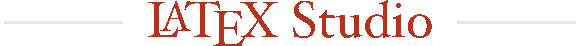
\includegraphics[width=7cm]{mcmthesis-logo}}}
\date{\today}

\renewcommand{\abstractname}{\vspace{-37.5pt}}

\memoto{Puzzle Editor of the New York Times}
\memofrom{Team \#2300466}
\memosubject{Research suggestions for Wordle answer words}
\memodate{\today}
%\memologo{\LARGE I'm pretending to be a LOGO!}

\begin{document}
\setcounter{tocdepth}{2}
\begin{abstract}
	
 Wordle, a small game with a simple drawing style, has recently gone viral. So that Wordle players are Posting or tweeting about their reports on various social platforms. In this paper, a variety of word attributes such as word frequency and information entropy are selected for modeling, so as to provide answers to the question and give some suggestions for the setting of the riddle.
 
For problem one, first, we corrected and eliminated the abnormal data.Considering that the data does not have the condition of time stationarity, we established the \textbf{Wordle Information Propagation Model} based on \textbf{Complex Network Propagation Dynamics}, and used \textbf{Attenuation Model} and other models to predict the future number of reports, and obtained the range of the number of reports on the same day as [17330,20900]. We combine \textbf{Information theory} and use \textbf{Word frequency}, \textbf{Information entropy} and other word attributes to quantify words. \textbf{Spearman} correlation analysis shows that the higher the Word frequency, Information Entropy and Popularity of a word, the higher the number of attempts. The higher the degree of repetition of the word letter, the lower the number of attempts.
	  
	For problem two, we used \textbf{Multiple stepwise regression}.Using word frequency, information entropy, popularity and other information as independent variables, the distribution of the number of attempts is analyzed by regression analysis. However, considering individual player differences, proficiency, Internet hot words and other uncertain factors, the model has a certain deviation. Compared with previous data, the average error of the model is less than  $\pm$ 2\%. The final predicted EERIE report scores were 0.38, 4.63, 15.86, 29.21, 27.91, 17.45, 5.46.   
	 
	 For problem three, we determined by the elbow rule that when the number of clustering centers is 3, the classification effect is optimal. The sample data is divided into three categories: difficult, medium and easy by \textbf{K-means} algorithm. According to the prediction of the word EERIE in question two, it is classified as "difficult". Finally, \textbf{BP neural network} classification algorithm is used to verify the classification results of the model, ensuring the accuracy of the classification evaluation model. 
	  
	  For problem four, in studying the above question, it was found that the number of hard mode reports as a percentage of the total number of players increased over time. We also found that the word part of speech had no effect on the difficulty of guessing. And we found that a more interesting phenomenon is that the number of times different letters appear in a puzzle can even affect the difficulty of the puzzle.
	  
\begin{keywords}
\textbf{Propagation Dynamics;\quad Entropy;\quad K-means;\quad Stepwise Regression}
\end{keywords}
\end{abstract}

\maketitle
%% Generate the Table of Contents, if it's needed.
\begin{spacing}{0.3}
	\tableofcontents
\end{spacing}
 \newpage
%%
%% Generate the Memorandum, if it's needed.


%%
\section{Introduction}
\subsection{Problem Background}

As a word guessing game, Wordle provides its players with an actual English word as a puzzle every day. Players were welcomed to guess the word in up to six attempts, using the change in tile color after submission as a cue.

Players can choose to play in Normal mode or Hard mode. The hard mode requires that once the player finds a correct letter in a word (the tiles are yellow or green), those words must be used in subsequent guesses. Given the numbers reported by many users on twitter, we did a regression analysis and forecast for the number of reported results, and built a rating model for the game words. According to the relevant characteristics of different words, the "difficulty" is classified, and the classification accuracy is discussed and analyzed.

\subsection{Restatement of the Problem}
\begin{itemize}
	\item Build a model to explain the change in the number of reported results and predict the range of reported results by March 1, 2023. Explore and explain how various word attributes affect the number of attempts.
	\item Given a certain date and daily puzzles, a model is built to predict the percentage of each attempt. And evaluate the advantages and disadvantages of the model.
	\item Establish a model, classify the difficulty of solving the problem according to the attributes of each word, and judge the difficulty category of EERIE words.
	\item Further explore other interesting features of the data set.
\end{itemize}

\subsection{Problem Analysis}

\textbf {For problem one:}

According to the data in the attachment, the time sequence chart of the Number of reported results since January 7, 2022 is drawn. It can be seen that the Number of reported results shows a trend of first rising and then declining over time. The Number of reported results also reflects the number of people who play the game, and given the nature of the game itself, we consider this phenomenon to be related to the life cycle of the game itself.

Therefore, several prediction models such as Broadbent-Treisman Parameter Model and Wordle information propagation model based on complex network propagation dynamics were established to predict and analyze the previous data. The number of reports is not only determined by time, but also needs to optimize the model by combining the word difficulty and the number of attempts distribution. Finally, the number of reports on March 1, 2023 is predicted to get the forecast range of the number of reports on that day.

In order to explore the influence of Word attributes on the number of attempts, we studied the correlation between Word Frequency, Information Entropy, Popularity and other attributes.
\begin{figure}[H]
	\centering
	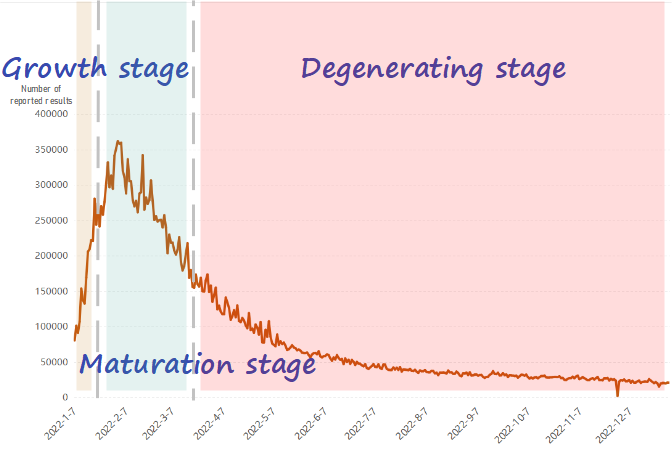
\includegraphics[width=.5\textwidth]{qw-1.png}
	\caption{\small Wordle life cycle}
\end{figure}

\textbf {For problem two:}

Firstly, an overall analysis of the data should be conducted. Kernel density estimation charts, scatter charts and histograms should be drawn for the percentages of different attempt times and word information entropy, word frequency and popularity. In order to avoid the influence of multicollinearity problem on the prediction model, multiple stepwise regression is selected for modeling. Word frequency, information entropy, popularity, number of letters, classification of repeated letters and other information were taken as independent variables, and the prediction model was obtained by stepwise regression of the percentage of different attempts. At the same time, the influence of uncertain factors on the model should be considered, and the effect of the model should be tested and analyzed to predict the percentage of different attempts of EERIE words.

\textbf {For problem three:}

In order to classify the riddle words according to the difficulty of guessing, we first plan to classify the sample data by K-means algorithm. After the classification of sample data, the difficulty is defined as the evaluation standard of vocabulary to conduct a more detailed quantitative analysis of the classification results. Combined with the prediction of each percentage of EERIE report results in question two, the difficulty is divided. Finally, the accuracy of classification results is verified by dividing training set and test set into sample data.


%
%\begin{table}[H]
%	\centering
%	\renewcommand\arraystretch{1.2}
%	\begin{tabular}{lcccc}
%		\toprule[1.5pt]
%		\makebox[0.05\textwidth][c]{} & \makebox[0.13\textwidth][c]{Coefficient} &	\makebox[0.13\textwidth][c]{SD} & \makebox[0.1\textwidth][c]{t} &
%	    \makebox[0.1\textwidth][c]{P\textgreater{}|t|} \\
%		\midrule[1.5pt]	
%		Constants  & -168.296  &463.874  & -0.363  & 0.717              \\
%		Number of results  & -0.362       & 0.049               & -7.337  & 0                  \\
%		\bottomrule[1.5pt]
%		
%		\multicolumn{5}{l}{\color{gray}{\footnotesize Note: ***, **, * represent 1\%, 5\%, 10\% significance levels}}
%	\end{tabular}
%\end{table}
%
%\begin{table}[H]
%	\centering
%	\caption{ADF Inspection}
%	\renewcommand\arraystretch{1.2}
%	\begin{tabular}{cccc}
%		\toprule[1.5pt]
%		\makebox[0.16\textwidth][c]{Difference order} &	\makebox[0.13\textwidth][c]{t} & \makebox[0.13\textwidth][c]{P} &
%		\makebox[0.13\textwidth][c]{AIC} \\
%		\midrule[1.5pt]	
%		0                                 & -3.921             & 0.002***           & 7191.855             \\
%		1                                 & -4.234             & 0.001***           & 7184.375             \\
%		2                                 & -10.788            & 0.000***           & 7164.178             \\
%		\bottomrule[1.5pt]
%		\multicolumn{4}{l}{\color{gray}{\footnotesize Note: ***, **, * represent 1\%, 5\%, 10\% significance levels}}             
%	\end{tabular}
%\end{table}

%\begin{table}[H]
%	\centering
%	\caption{\small Letter Frequency}
%	\renewcommand\arraystretch{1.2}
%	\begin{tabular}{cc}
%		\toprule[1.5pt]
%		\makebox[0.25\textwidth][c]{Methods} & \makebox[0.25\textwidth][c]{Gradual} \\
%		\midrule[1.5pt]
%		Reserved Variables & \begin{tabular}[c]{@{}c@{}}
%			$C \quad F\quad P\quad L_t\quad L_p\quad L_h\quad L_y$ \\ $L_e\quad L_w\quad E\quad L_d\quad L_l\quad L_v\quad L_g$ \end{tabular} \\
%		Discard Variables & \begin{tabular}[c]{@{}c@{}} $L_a\quad L_b\quad L_c\quad L_f\quad L_j\quad L_k\quad L_l\quad L_m$ \\ $L_n\quad L_o\quad L_q\quad L_r\quad L_s\quad L_u\quad L_x\quad L_z$ \end{tabular} \\
%		\bottomrule[1.3pt]
%	\end{tabular}
%\end{table}

%\begin{eqnarray}
%	E(I)  =  -\sum_{x} p\left(x\right) \cdot \log _{2} p\left(x\right)
%\end{eqnarray}
%
%\begin{eqnarray}
%	\operatorname{sigmoid}(z) = \frac{1}{1+e^{-z}}
%\end{eqnarray}

%\begin{Theorem} \label{thm:latex}
%\LaTeX
%\end{Theorem}
%\begin{Lemma} \label{thm:tex}
%\TeX .
%\end{Lemma}
%\begin{proof}
%The proof of theorem.
%\end{proof}

\section{General Assumptions and Notations}

\subsection{Assumptions}
\begin{itemize}
	\item Assume a positive linear correlation between the number of reports and the number of actual visitors.
	\item Assume that all twitter users are likely to see the game.
	\item Assume that there is little difference in individual word cognition.
%	\item Assume that only the characteristics of the words themselves are considered, excluding the influence of Internet celebrity effect or other unknown factors on the result prediction
\end{itemize}

\subsection{Notations}
\begin{table}[H]
	\centering
	\renewcommand\arraystretch{1.1}
	\begin{tabular}{cc}
		\toprule[1.5pt]
		\makebox[0.3\textwidth][c]{Symbol}	&  \makebox[0.4\textwidth][c]{Description} \\
		\midrule[1pt]
		$ N $	    	& Twitter user numbers   \\ 
		$ S(t) $	    	& Untouched game users\\  
		$ E(t) $	    	& Temporarily unplayed players  \\ 
		$ I(t) $	        & Players who are playing\\ 
		$ R(t) $		& Players who give up \\ 
		$ Rnum(t) $		& Number of reports for the day \\ 
		$ Dif(t) $			& Average number of attempts for the day \\ 
		$ Try_2(t) $	    	& Percentage of two attempts for the day\\  
		$ \beta  $	    	& Probability of seeing a tweet tour  \\ 
		$ \sigma $	        & Return rate of old players\\ 
		$ \gamma $		& Player departure rate \\ 
		$ k $		& Propagation rate of tweets \\ 
		$ z $			& Probability of sending tweets \\ 
		\bottomrule[1.5pt]
	\end{tabular}
\end{table}

\section{Analysis and prediction of Number of reported results}
\subsection{Data preprocessing}

Data availability must be ensured before data analysis. Firstly, we cleaned the data in the attachment and modified and eliminated individual outliers.

\subsubsection{Modification of abnormal words}
Through search all data, according to Wordle game rules, the basis of word length should be five. Therefore, we will select the words whose length does not conform to five and replace them with correct words by comparing the data on Wordle's official website with the known data of the title. The replacement result is as follows:
\begin{table}[H]
	\centering
	\renewcommand\arraystretch{1.2}
	\caption{\small Correlation result}
	\begin{tabular}{ccc}
		\toprule[1.5pt]
		\makebox[0.2\textwidth][c]{Contest number} & \makebox[0.25\textwidth][c]{Abnormalword} 
		& \makebox[0.2\textwidth][c]{Revised} \\
		\midrule[1.5pt]
		314 & tash & trash \\
		525 & clen & clean \\
		545 & rprobe & probe \\
		\bottomrule[1.5pt]
	\end{tabular}
\end{table}
\subsubsection{Correction of abnormal values}
By calculating the percentage of players in hard mode as a percentage of all players with Contest number of 529 words, we clearly find that the percentage of players participating in hard mode as a percentage of all players is significantly outlier than the other sample data.
\begin{figure}[H]
	\centering
	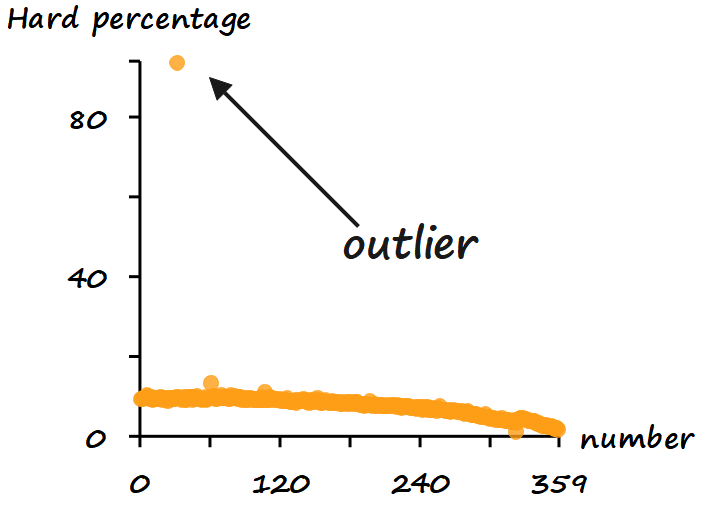
\includegraphics[width=.6\textwidth]{Q1-yczcl.png}
	\caption{\small Outlier scheme}
\end{figure}

And then we treat that as an outlier. Combined with the data of the first and second days, the interpolation algorithm was used to complete 25569, and the correction was completed.
\subsubsection{Delete abnormal data}
Given that they're saying that the percentage plus the number of attempts a player makes may differ a little bit from 100\% because of some calculation error. After we checked all the data, we found that except for the data with Contest number 281, the number of attempts added up to 126\%, the rest of the data was within the range of 100\%$\pm$2\%. Therefore, it is regarded as statistical error and excluded as outlier.
At this point, the preprocessing of the data given in this question is over.

\subsection{Establishment of model}
Contest number is an index of the Wordle puzzles, so Contest number can be regarded as a sequence that has no effect on the data. We plot the number of reported results by Contest number as a scatter plot and plot the overall trend of the data growing with Contest number. It can be seen that the Number of reported results reached a peak in early February. As the number of contests grows, the Number of reported results in the future decreases. Below is the kernel density estimate (KDE) graph, and the linear regression residual graph.
\begin{figure}[H]
	\subfigure
	{
		\begin{minipage}[b]{.28\linewidth}
			\centering
			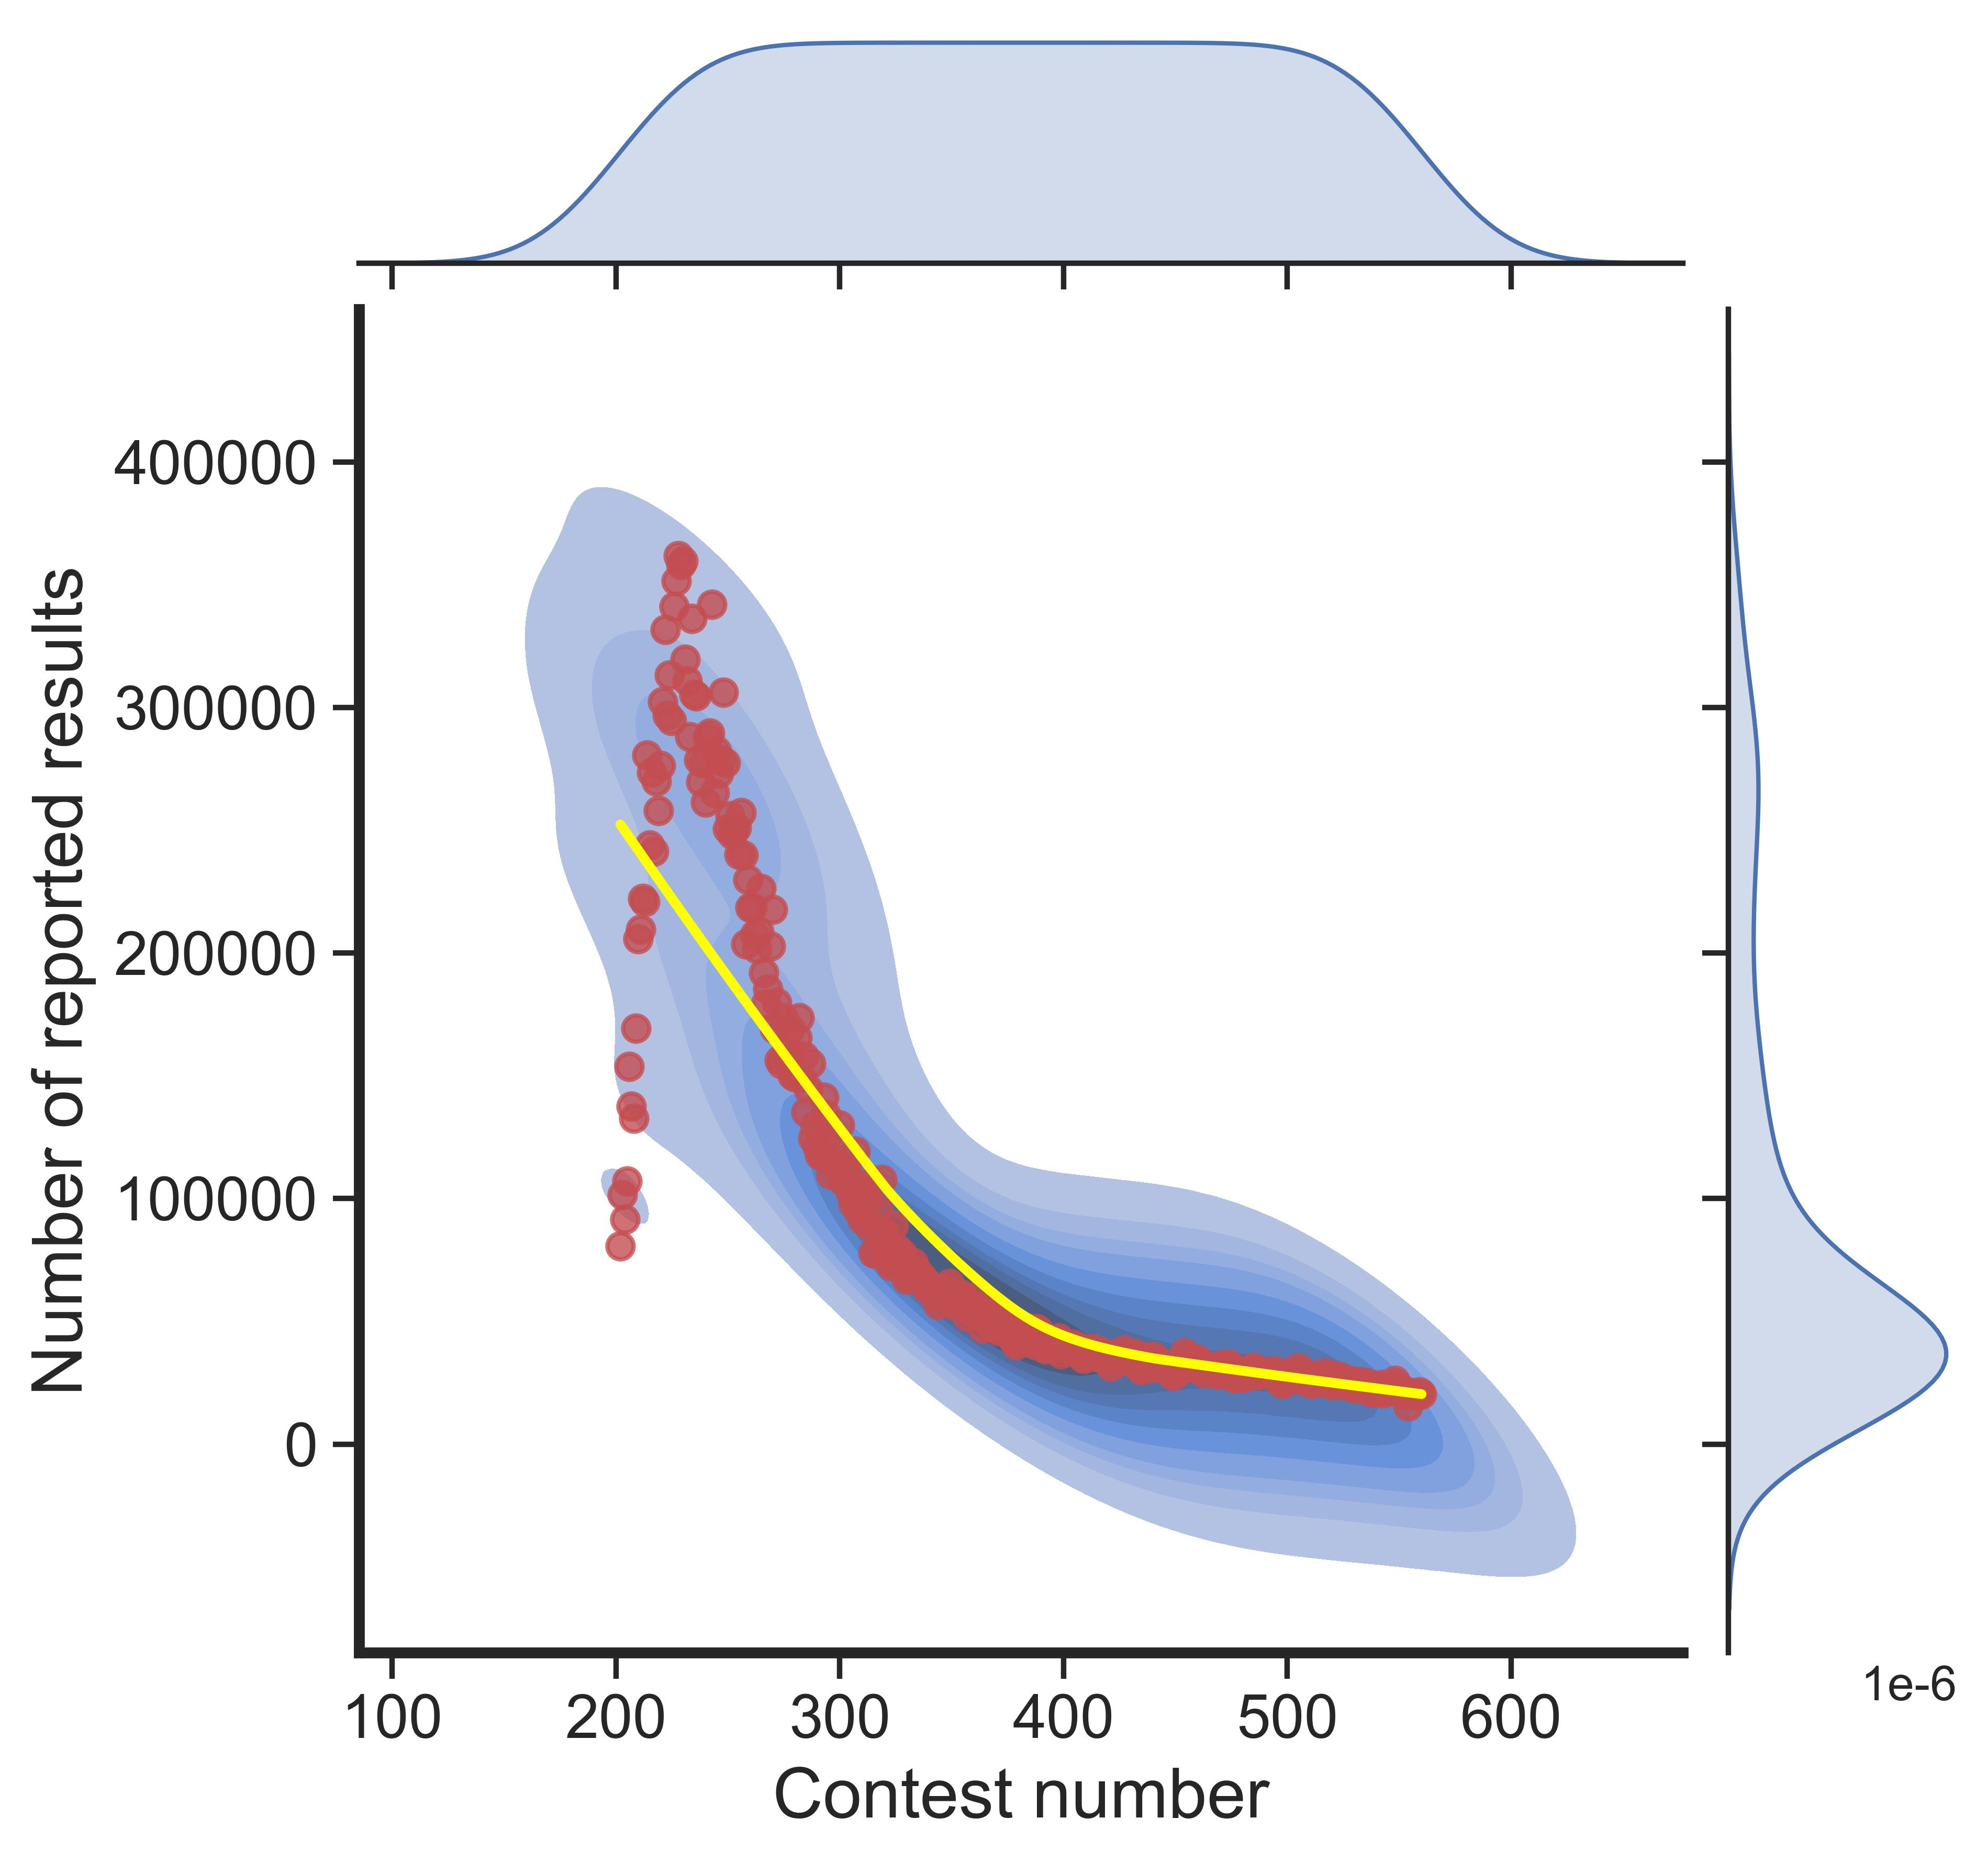
\includegraphics[scale=0.43]{Number_of_reported_results_kde.jpg}
		\end{minipage}
	} \quad \quad \quad \quad \quad \quad \quad 
	\subfigure
	{
		\begin{minipage}[b]{.28\linewidth}
			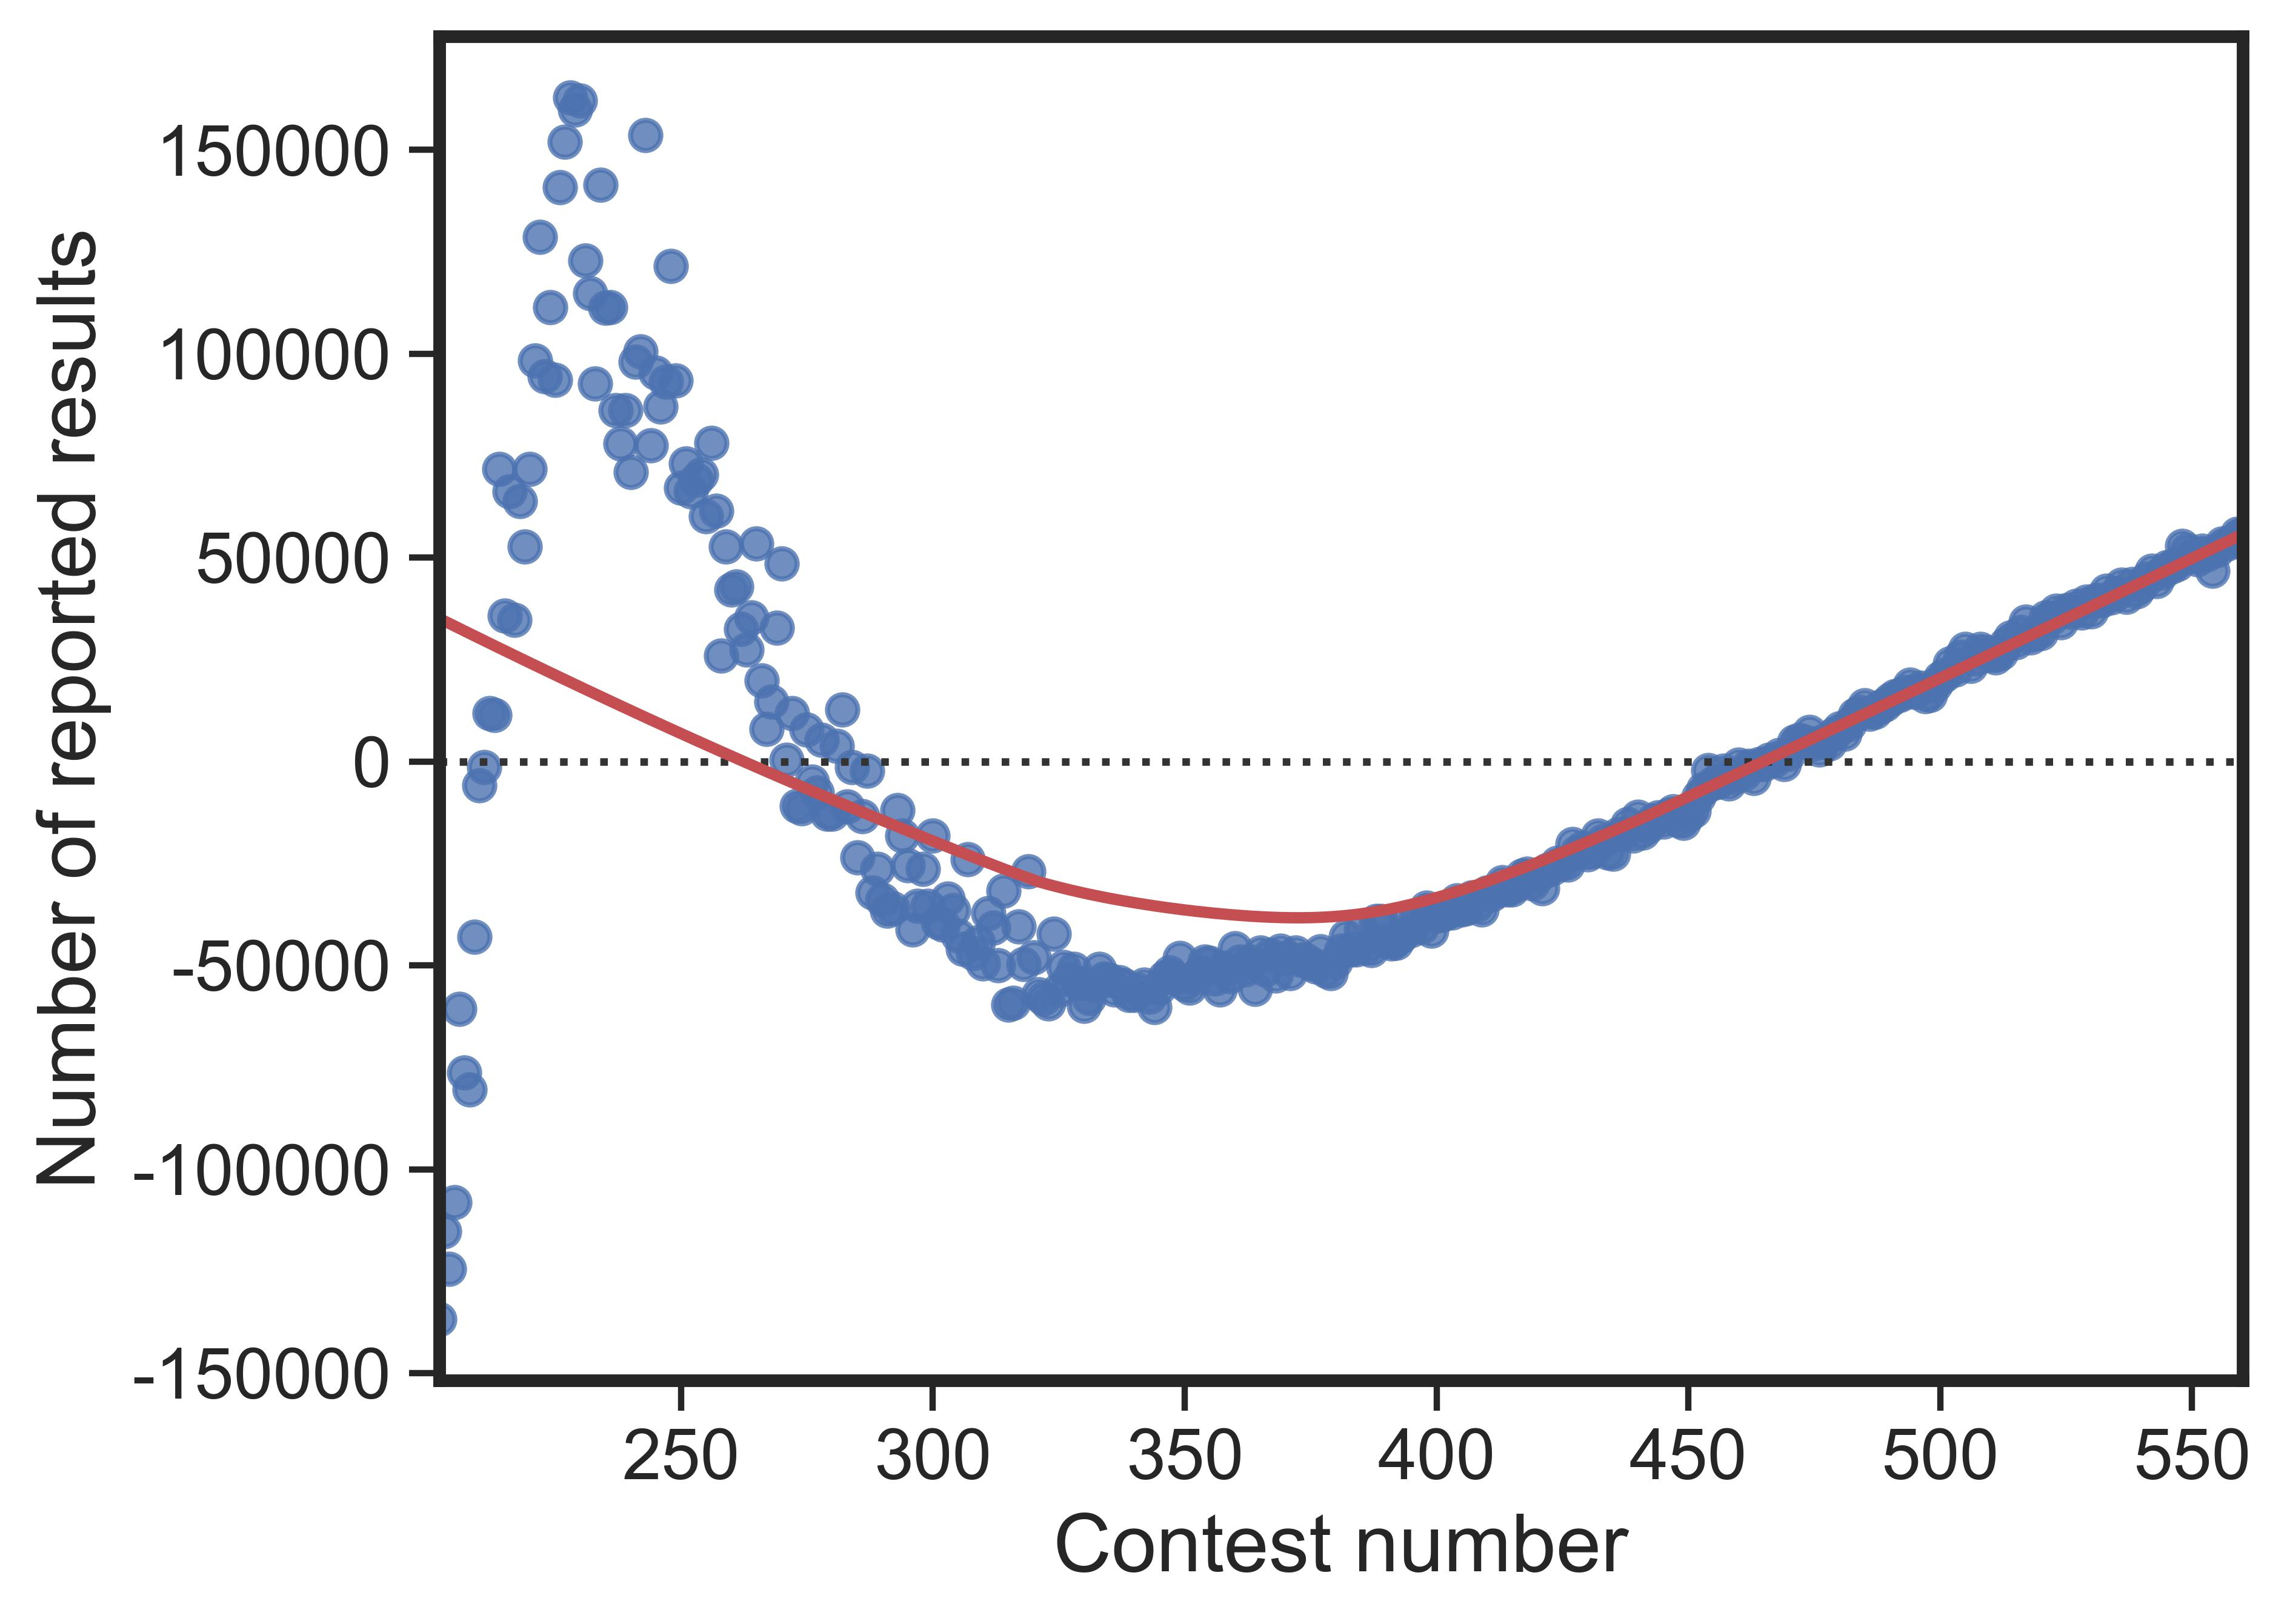
\includegraphics[scale=0.45]{Number_of_reported_results_resid.jpg}
		\end{minipage}
	}
\end{figure}

As can be seen from the information in the chart above, the Number of reported result is not simply a set of time-series meaningful data, but something deeper. So we can analyze and predict it using the Broadbent-Treisman parameter Model, complex network propagation dynamics model and other mathematical models.

\subsubsection{Broadbent-Treisman Attenuation Model}
The traditional filter model is the process of radio wave being blocked by different substances in space propagation, which leads to the blocking of signal. Treisma improved the model and proposed a attenuation model, which believes that the filter does not only allow the information of one channel to pass through, but also the information of other channels can be weakened by just being attenuated.
\begin{figure}[H]
	\centering
	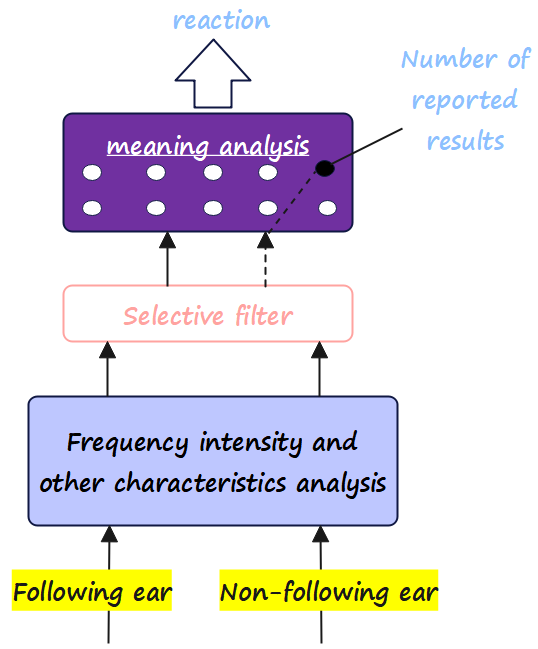
\includegraphics[width=.42\textwidth]{Q1-lct1.png}
	\caption{\small Attenuation model flow}
\end{figure}

We define Wordle player $a$ to tweet the guess data as event $q$, and the effect of $q$ on player $a$ is $u$, discuss the average influence of $q$ on society $T_q$.

If the probability that a random user $b$ sees the post and becomes interested in it is $r \in (0,1)$, then the information decays as $f(r)=e^{-\eta  r}$ times when propagating from $a$ to $b$.

Then the impact on person $b$ is:	
\begin{eqnarray}
	T_a(b)=f(r)u
\end{eqnarray}

By abstracting player $a$ as a point $a^*$ on the plane, we can assume that society is a unit circle O centered at point $a^*$, with all people evenly distributed on the surface. Since the probability of player $a$'s tweet being seen by any other user is relatively average, the average influence of each person can be used to represent the influence of event $q$ on society. That is:
\begin{eqnarray}
	T_{q}  =  \frac{\int_{0} u f(r) d_0}{\pi}  =  u \int_{0}^{1} f(r) d r
\end{eqnarray}

Furthermore, the above information attenuation model was used to simulate the change of the Number of reported results. The exponential smoothing method was used to predict and fit the attenuation trend of the Number of reported results, and the goodness of fit was 0.91. It shows that the fitting effect of the model is good.
%\begin{table}[H]
%	\centering
%	\renewcommand\arraystretch{1.2}
%	\caption{\small Model stats table}
%	\begin{tabular}{ccc}
%		\toprule[1.5pt]
%		\multicolumn{3}{c}{Model Stats} \\ 
%		\midrule[1.5pt]
%		\makebox[0.15\textwidth][c]{Model} &
%		\makebox[0.08\textwidth][c]{} & \makebox[0.15\textwidth][c]{Stable R-squared} \\
%		Number of reported  & & 0.915     \\  
%		\bottomrule[1.5pt]
%	\end{tabular}
%\end{table}

\subsubsection{Wordle Information Propagation Model based on Complex Network Propagation Dynamics}
The problem calls for a more reasonable explanation of the daily variation in the number of reported results. We built a network information propagation model for Wordle games to explain the changes in the reported quantity in the existing data, so as to predict the future quantity changes.

The spread of a game or piece of information goes through periods of growth, maturity, decline, and stability. The reported number is the number of Wordle players who played and tweeted that day. We believe that the number of tweets is mainly affected by the number of players, and that more tweets attract more players. Therefore, we establish Wordle information propagation model based on complex network propagation dynamics.

When the average Twitter user sees a tweet about the game, there is a $\beta\%$ chance that they will choose to become a new Wordle player. When a player plays a game, he will send a tweet report $z\%$ of the time and become a regular player. Potential players have a $\sigma\%$ chance of returning to play, or a $ \gamma\%$ chance of leaving after multiple plays. The flow chart of information dissemination is as follows:
\begin{figure}[H]
	\centering
	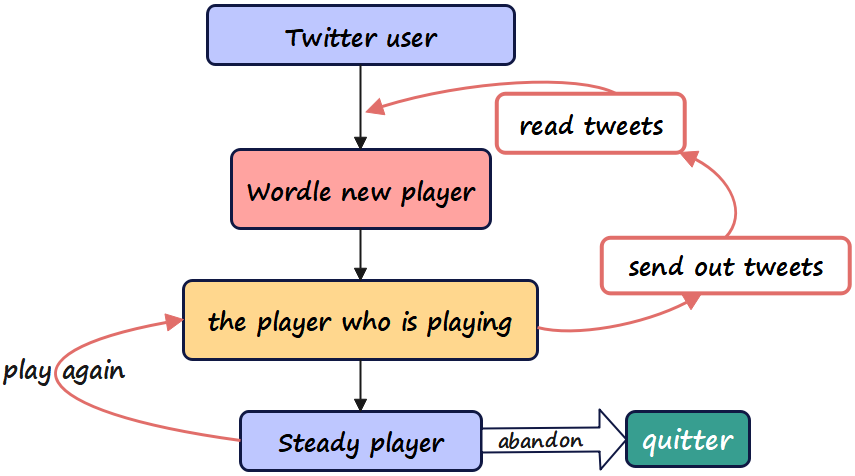
\includegraphics[width=.7\textwidth]{Q1-lct2.png}
	\caption{\small Wordle information propagation dissemination process}
\end{figure}
The parameter relationship of each variable is as follows:
\begin{eqnarray}
	\begin{aligned}
		&	 N  = S+E+I+R \\
		&	\frac{d S(t)}{d t} = -\frac{\beta S(t) I(t)}{N} \\
		&	\frac{d E(t)}{d t} = \frac{\beta S(t) I(t)}{N}-\sigma E(t) \\
		&	\frac{d I(t)}{d t} = \sigma E(t)-\gamma I(t) \\
		&	\frac{d R(t)}{d t} = \gamma I(t)
	\end{aligned}	
\end{eqnarray}
\qquad The number of daily reports can be obtained through calculation:
\begin{eqnarray}
	\label{Rnum}
	Rnum(t)=zI(t)
\end{eqnarray}
\qquad By fitting the original data, the original model is obtained through multiple fitting.See appendix for its initial parameters:

After visualizing the number of reports, we can intuitively find that there are significant fluctuations in the number of daily reports. It fluctuates for reasons that cannot be explained by time t. We further analyzed the data and found that the larger the percentage of the first three attempts on the day, the more significant the fluctuation in the number of reports on the day. So we assume that the number of daily reports fluctuates in relation to word difficulty.

To further verify the conjecture, $Dif(t)$ is calculated, and correlation analysis is made between it and $Rnum(t-1)*Rnum(t)$. They were found to be significantly correlated, and $Try_2(t)$ was the most correlated.

From this analysis, we can conclude that the fewer attempts a player takes to complete a game, the more likely they are to send a tweet.

In the Wordle information propagation model, the number of attempts and the probability $z$ of sending tweets have an effect. Therefore, we establish the probability evaluation equation with $Dif(t)$ as the basis and $Try_2(t)$ as the disturbance term:
\begin{eqnarray}
	z  = \frac{\operatorname{Dif}(t)+\operatorname{sigmoid}\left(T r y_{2}(t)-0.5\right)}{10}
\end{eqnarray}
\qquad Combined formula\ref{Rnum}:
\begin{eqnarray}
	Rnum(t) = \frac{\operatorname{Dif}(t)+\operatorname{sigmoid}\left(T r y_{2}(t)-0.5\right)}{10}I(t)
\end{eqnarray}
\qquad According to the Wordle information propagation model, the Fitting Graph and the APE Graph are obtained. It can be seen that the fitting degree is excellent, and MAPE is 9.892.
\begin{figure}[H]
	\subfigure
	{
		\begin{minipage}[b]{.28\linewidth}
			\centering
			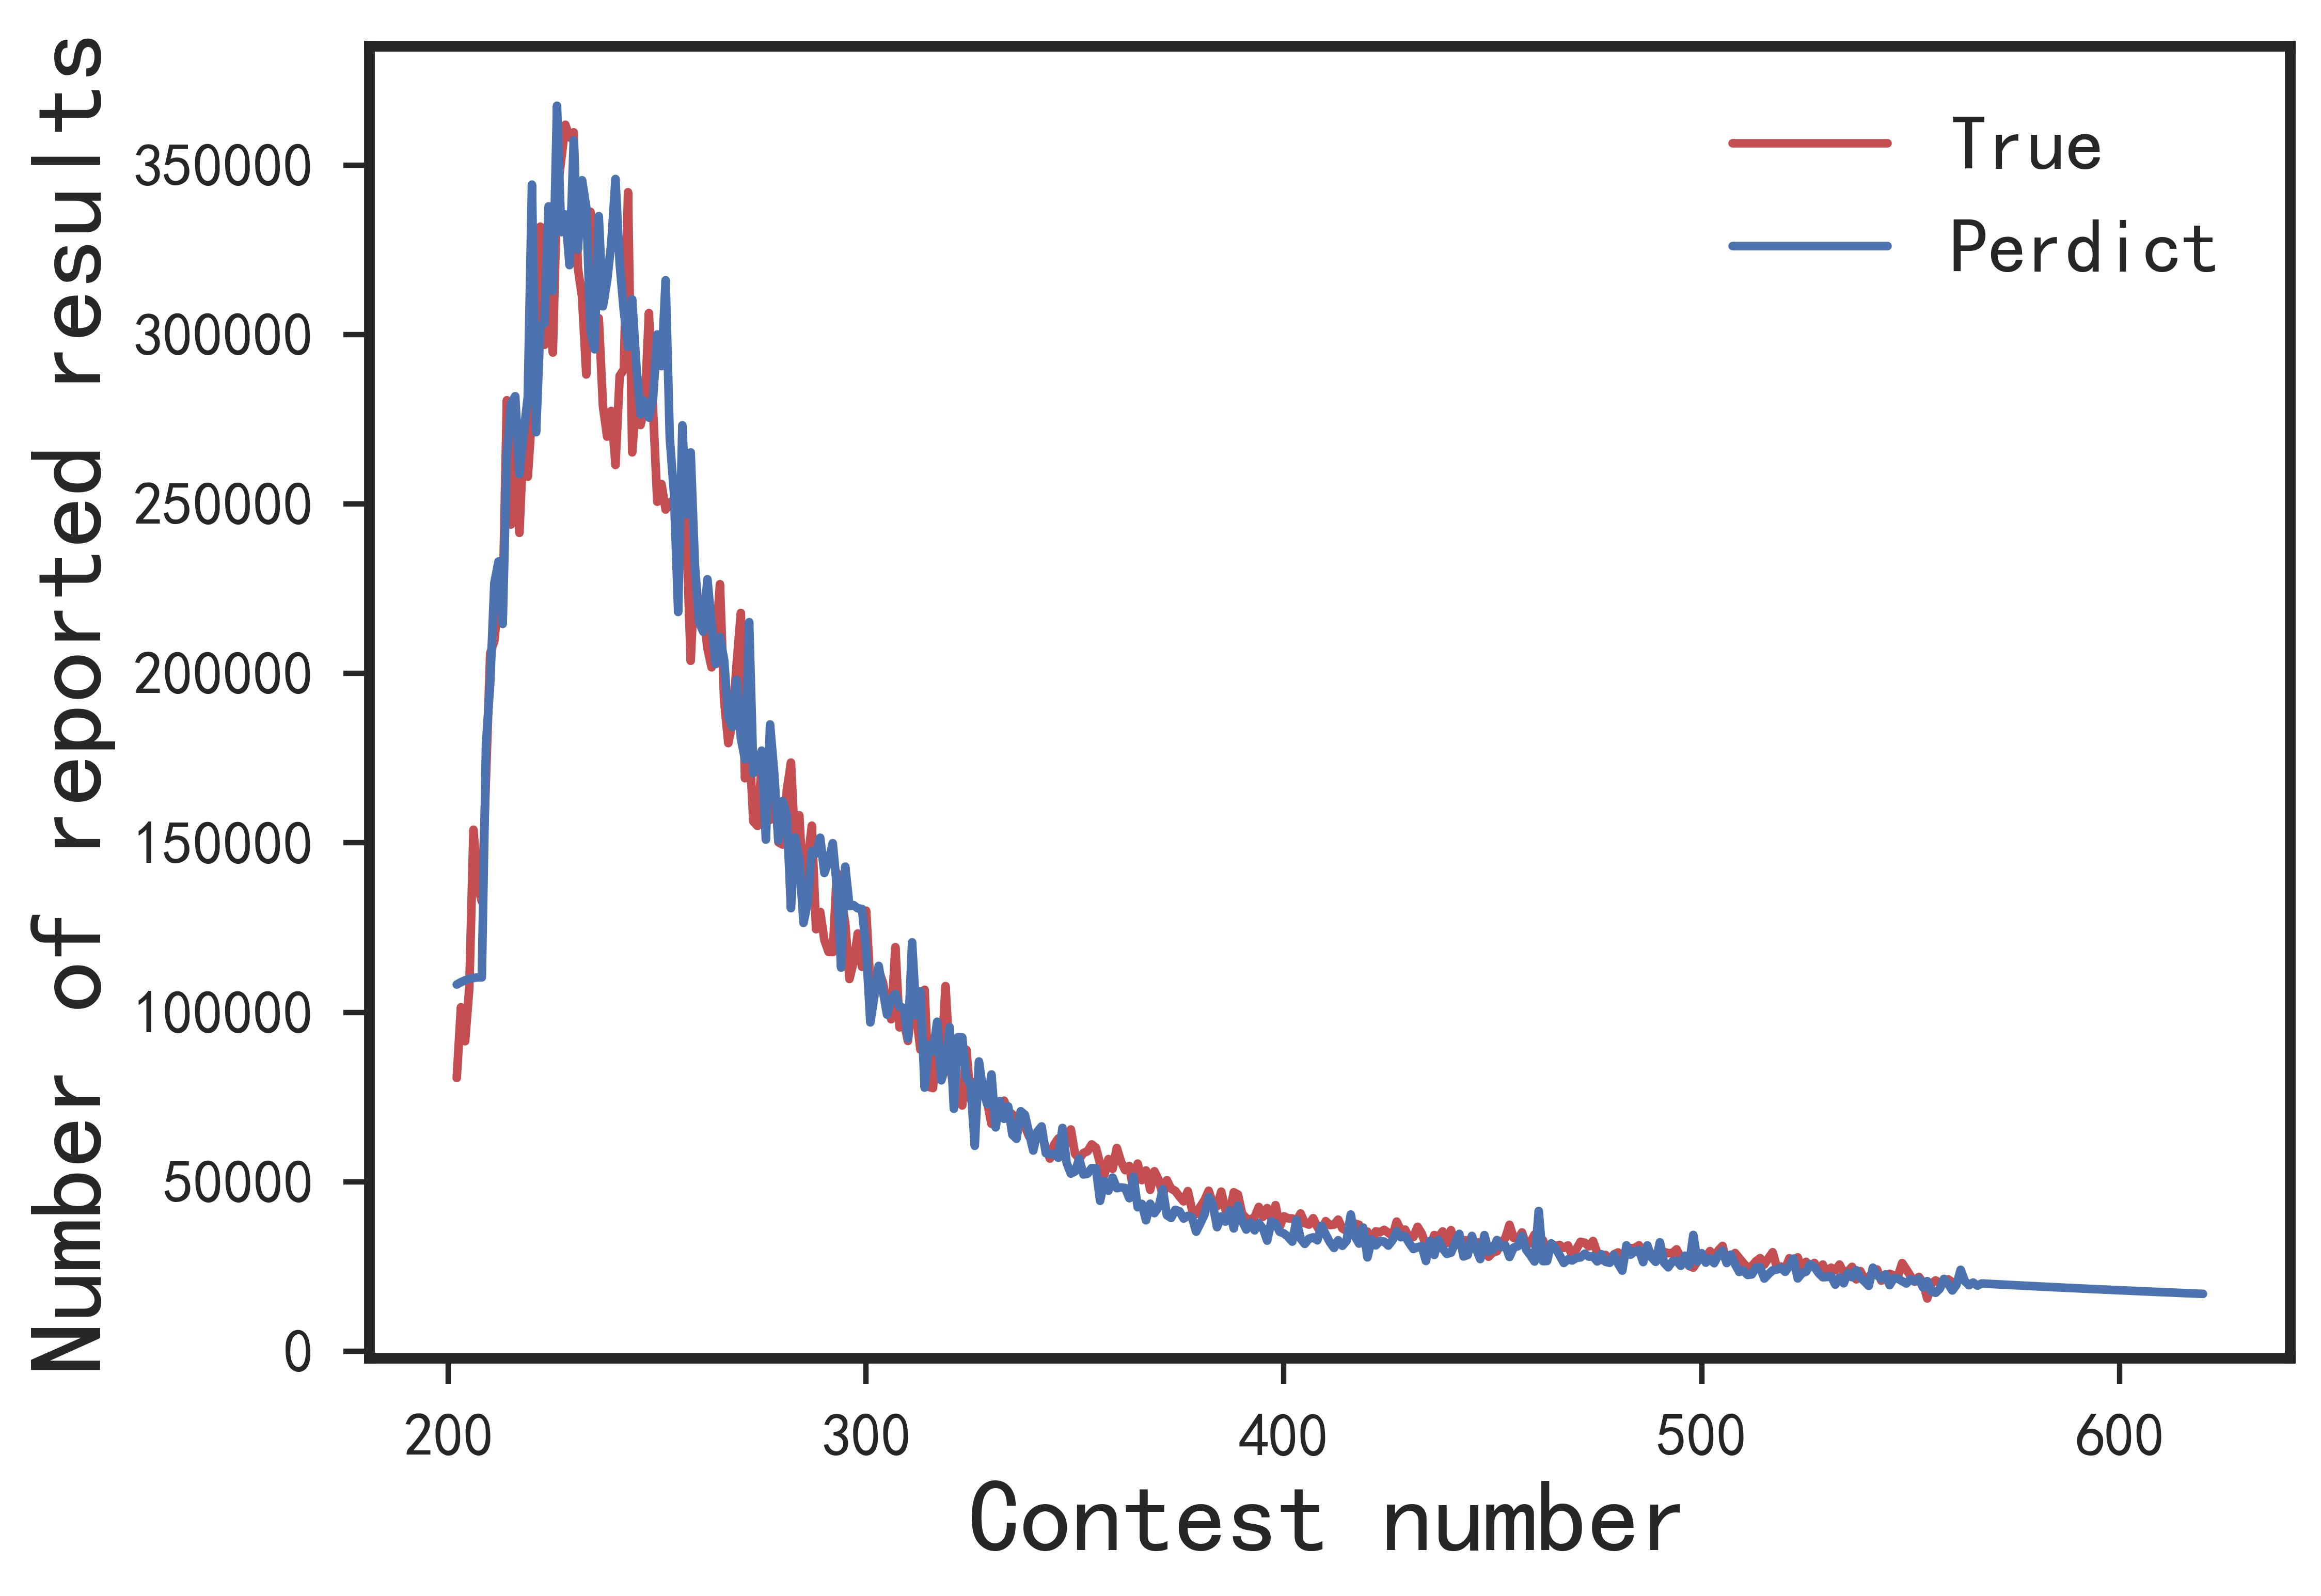
\includegraphics[scale=0.38]{Wordle_progration_perdict.jpg}
		\end{minipage}
	} \quad \quad \quad \quad \quad \quad \quad 
	\subfigure
	{
		\begin{minipage}[b]{.28\linewidth}
			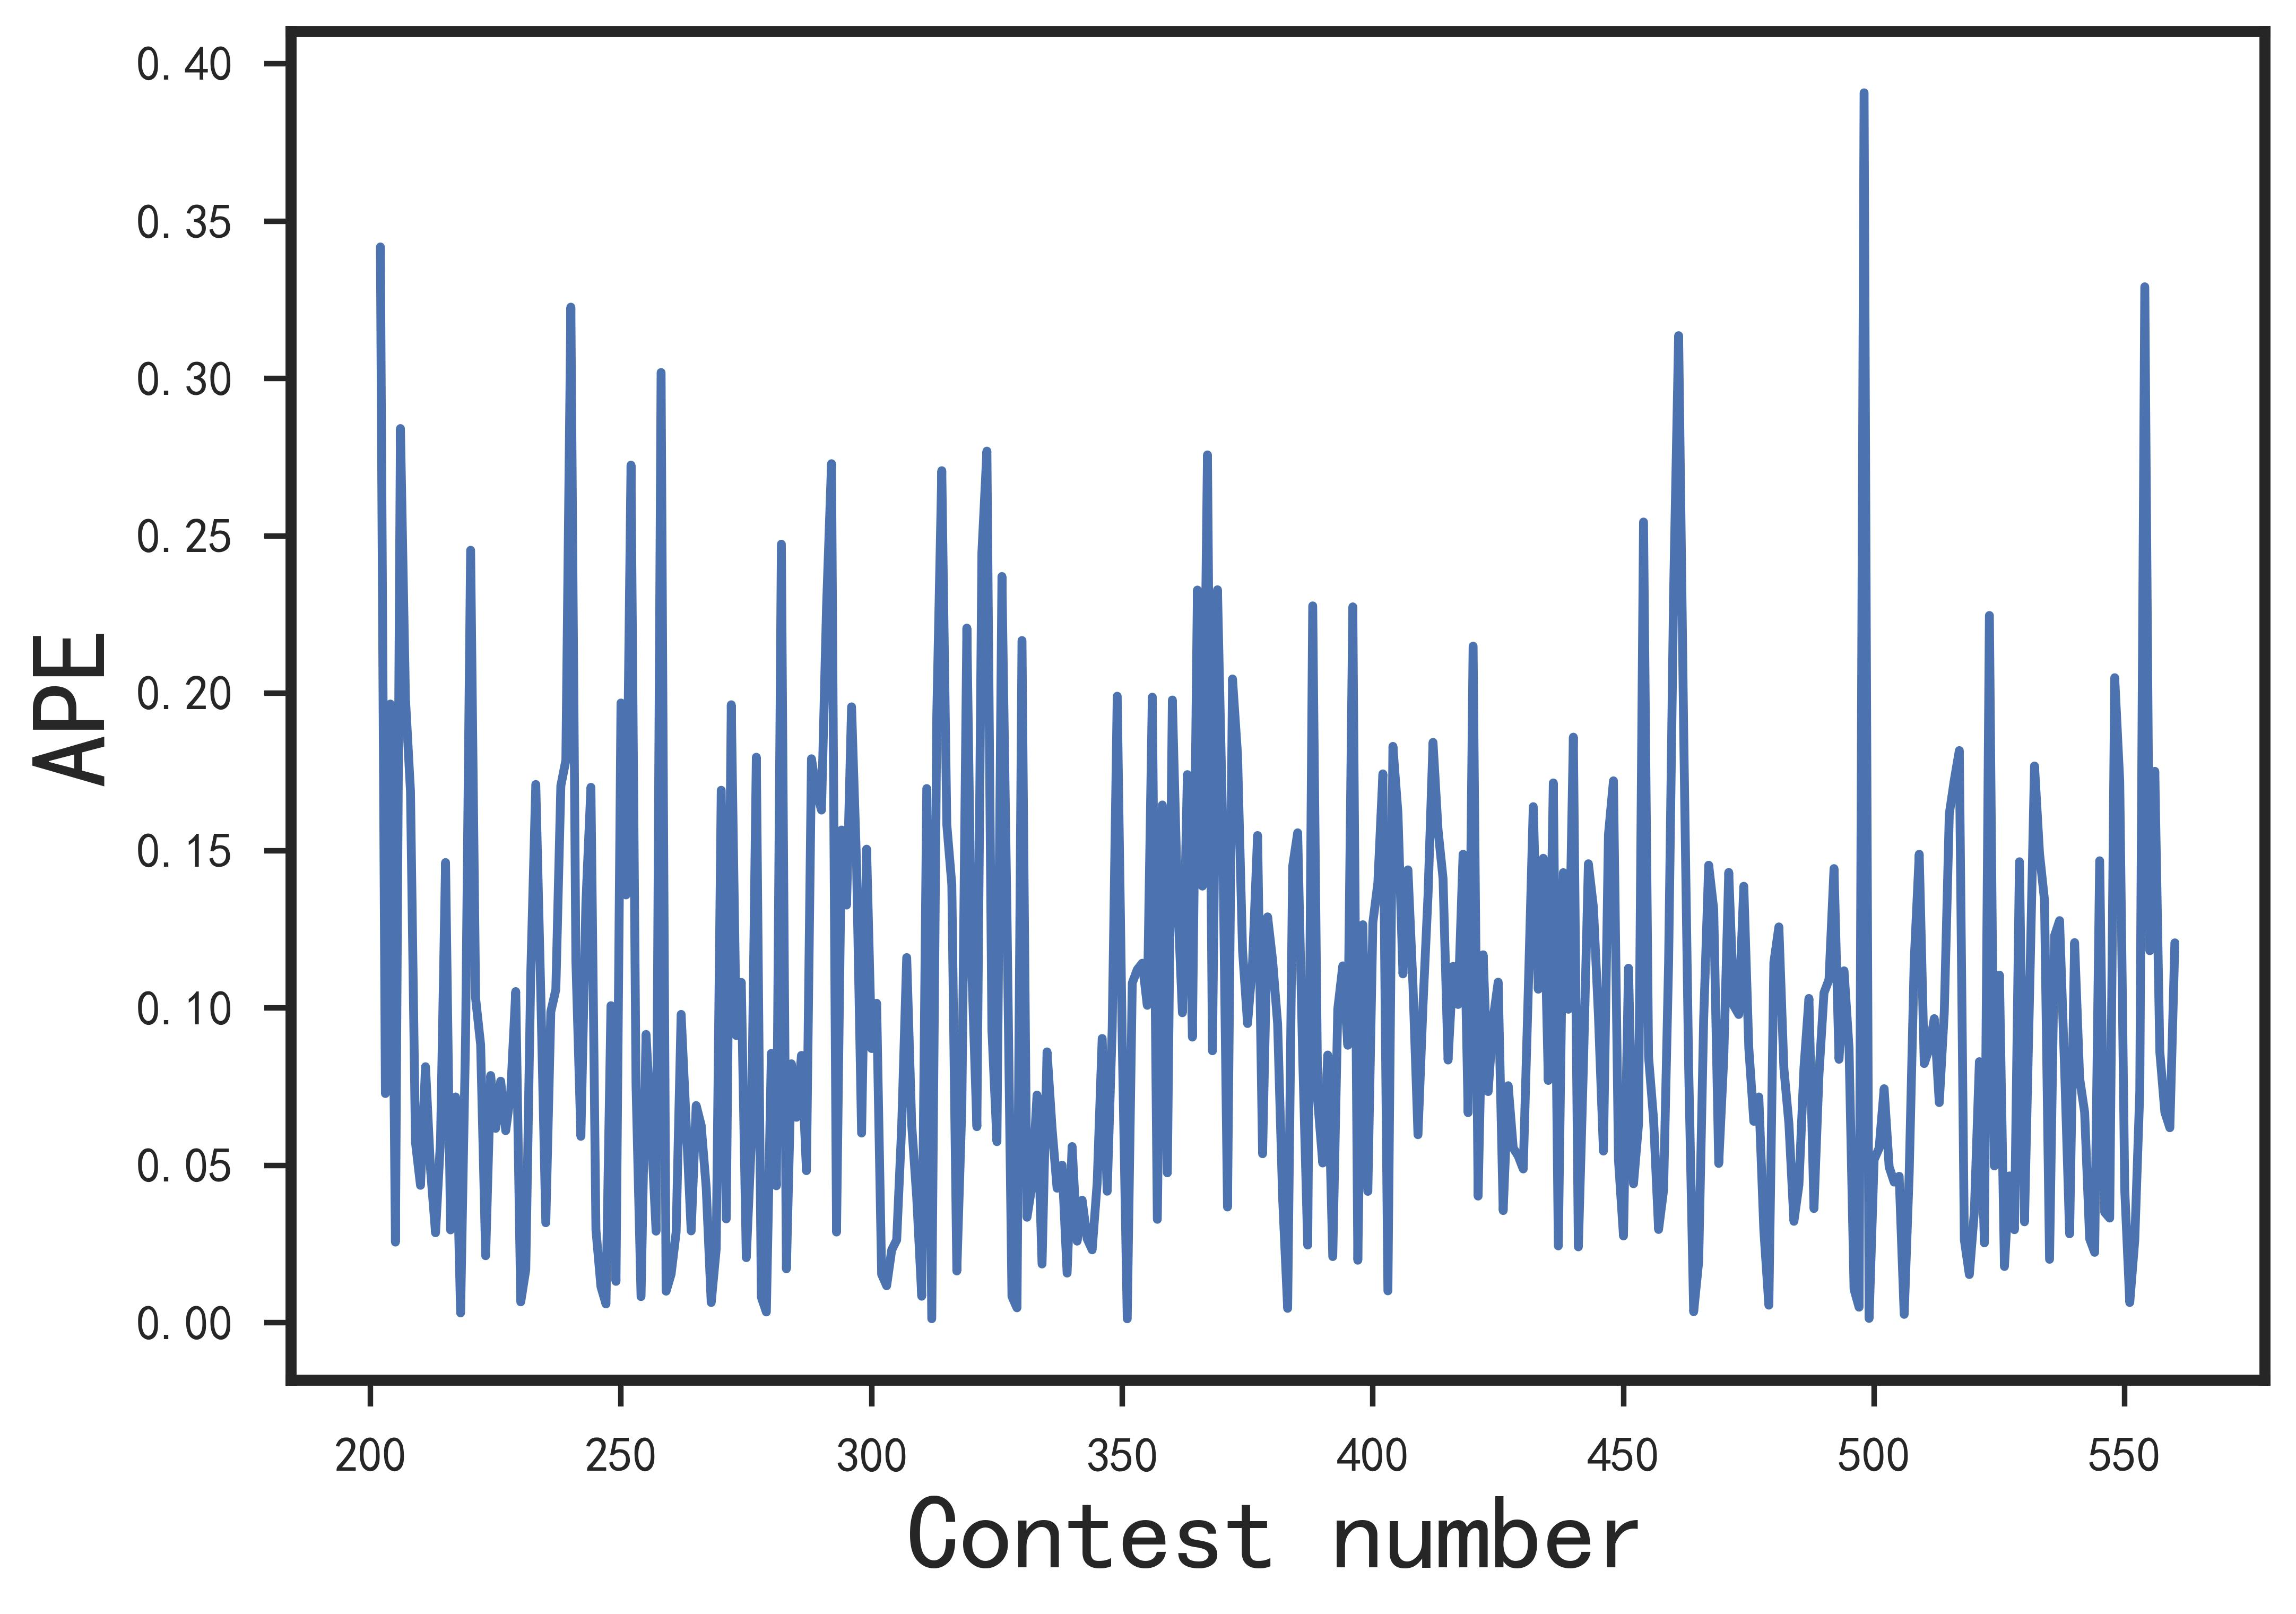
\includegraphics[scale=0.38]{Wordle_progration_APE.jpg}
		\end{minipage}
	}
\end{figure}

%\subsubsection{Analysis and prediction of other models}
%After the prediction of the above model, in order to make the analysis more perfect, we used the ARIMA model, LSTM algorithm and XGB algorithm to predict the number of reported result. The following is the prediction graph of the MAPE of these algorithms and the test set.
%\begin{figure}[H]
%	\centering
%	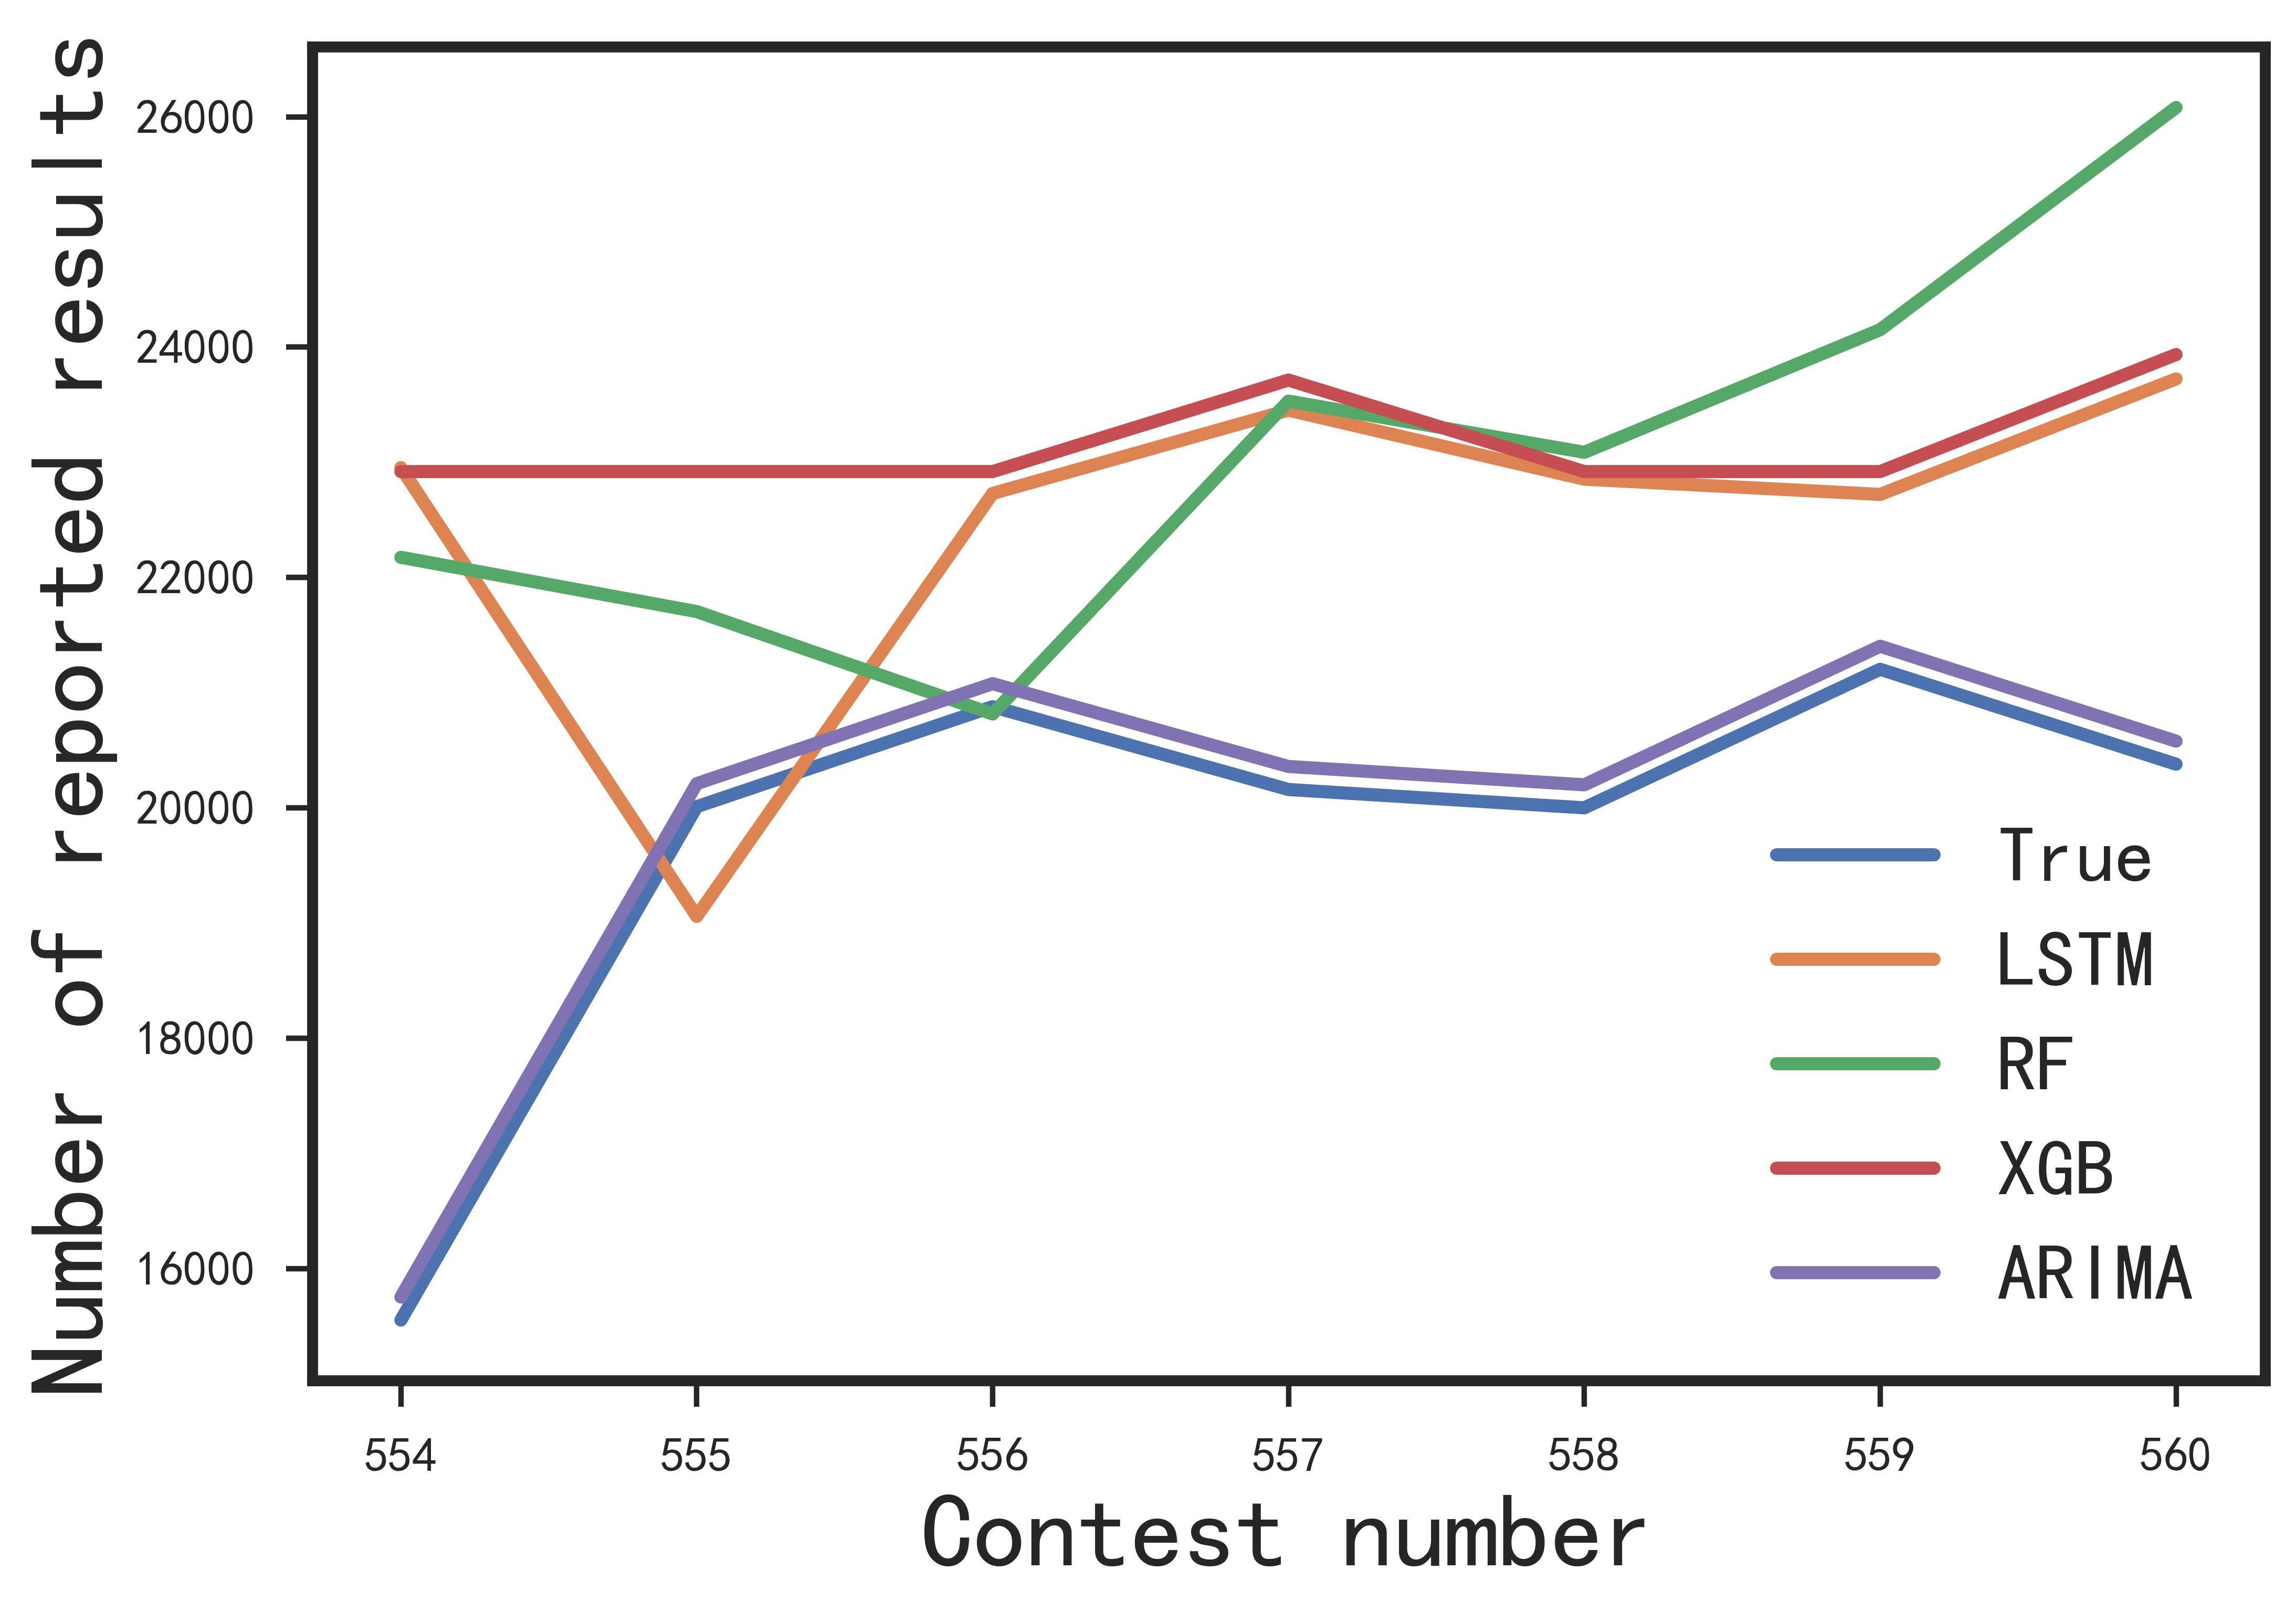
\includegraphics[width=.6\textwidth]{LSTM_test.jpg}
%\end{figure}
%
%\begin{table}[H]
%	\centering
%	\caption{\small Letter Frequency}
%	\renewcommand\arraystretch{1.2}
%	\begin{tabular}{cc}
%		\toprule[1.5pt]
%		\makebox[0.25\textwidth][c]{Algorithm} & \makebox[0.25\textwidth][c]{MAPE} \\
%		\midrule[1.5pt]
%		LSTM & 13.241 \\
%		XGBoost & 13.556 \\
%		RandomForest & 13.232 \\
%		\bottomrule[1.3pt]
%	\end{tabular}
%\end{table}

\subsubsection{Model summary and interval prediction}
After the prediction of the above model, we used ARIMA model, LSTM algorithm and XGB algorithm to predict the number of reported results in order to make the analysis more perfect. By comparing the confidence intervals of the various models, it is obtained that the number interval of reported results on March 1, 2023 is [17330,20900] at the 95 percent confidence level. Below is the forecast result graph of the five different models.
\begin{figure}[H]
	\centering
	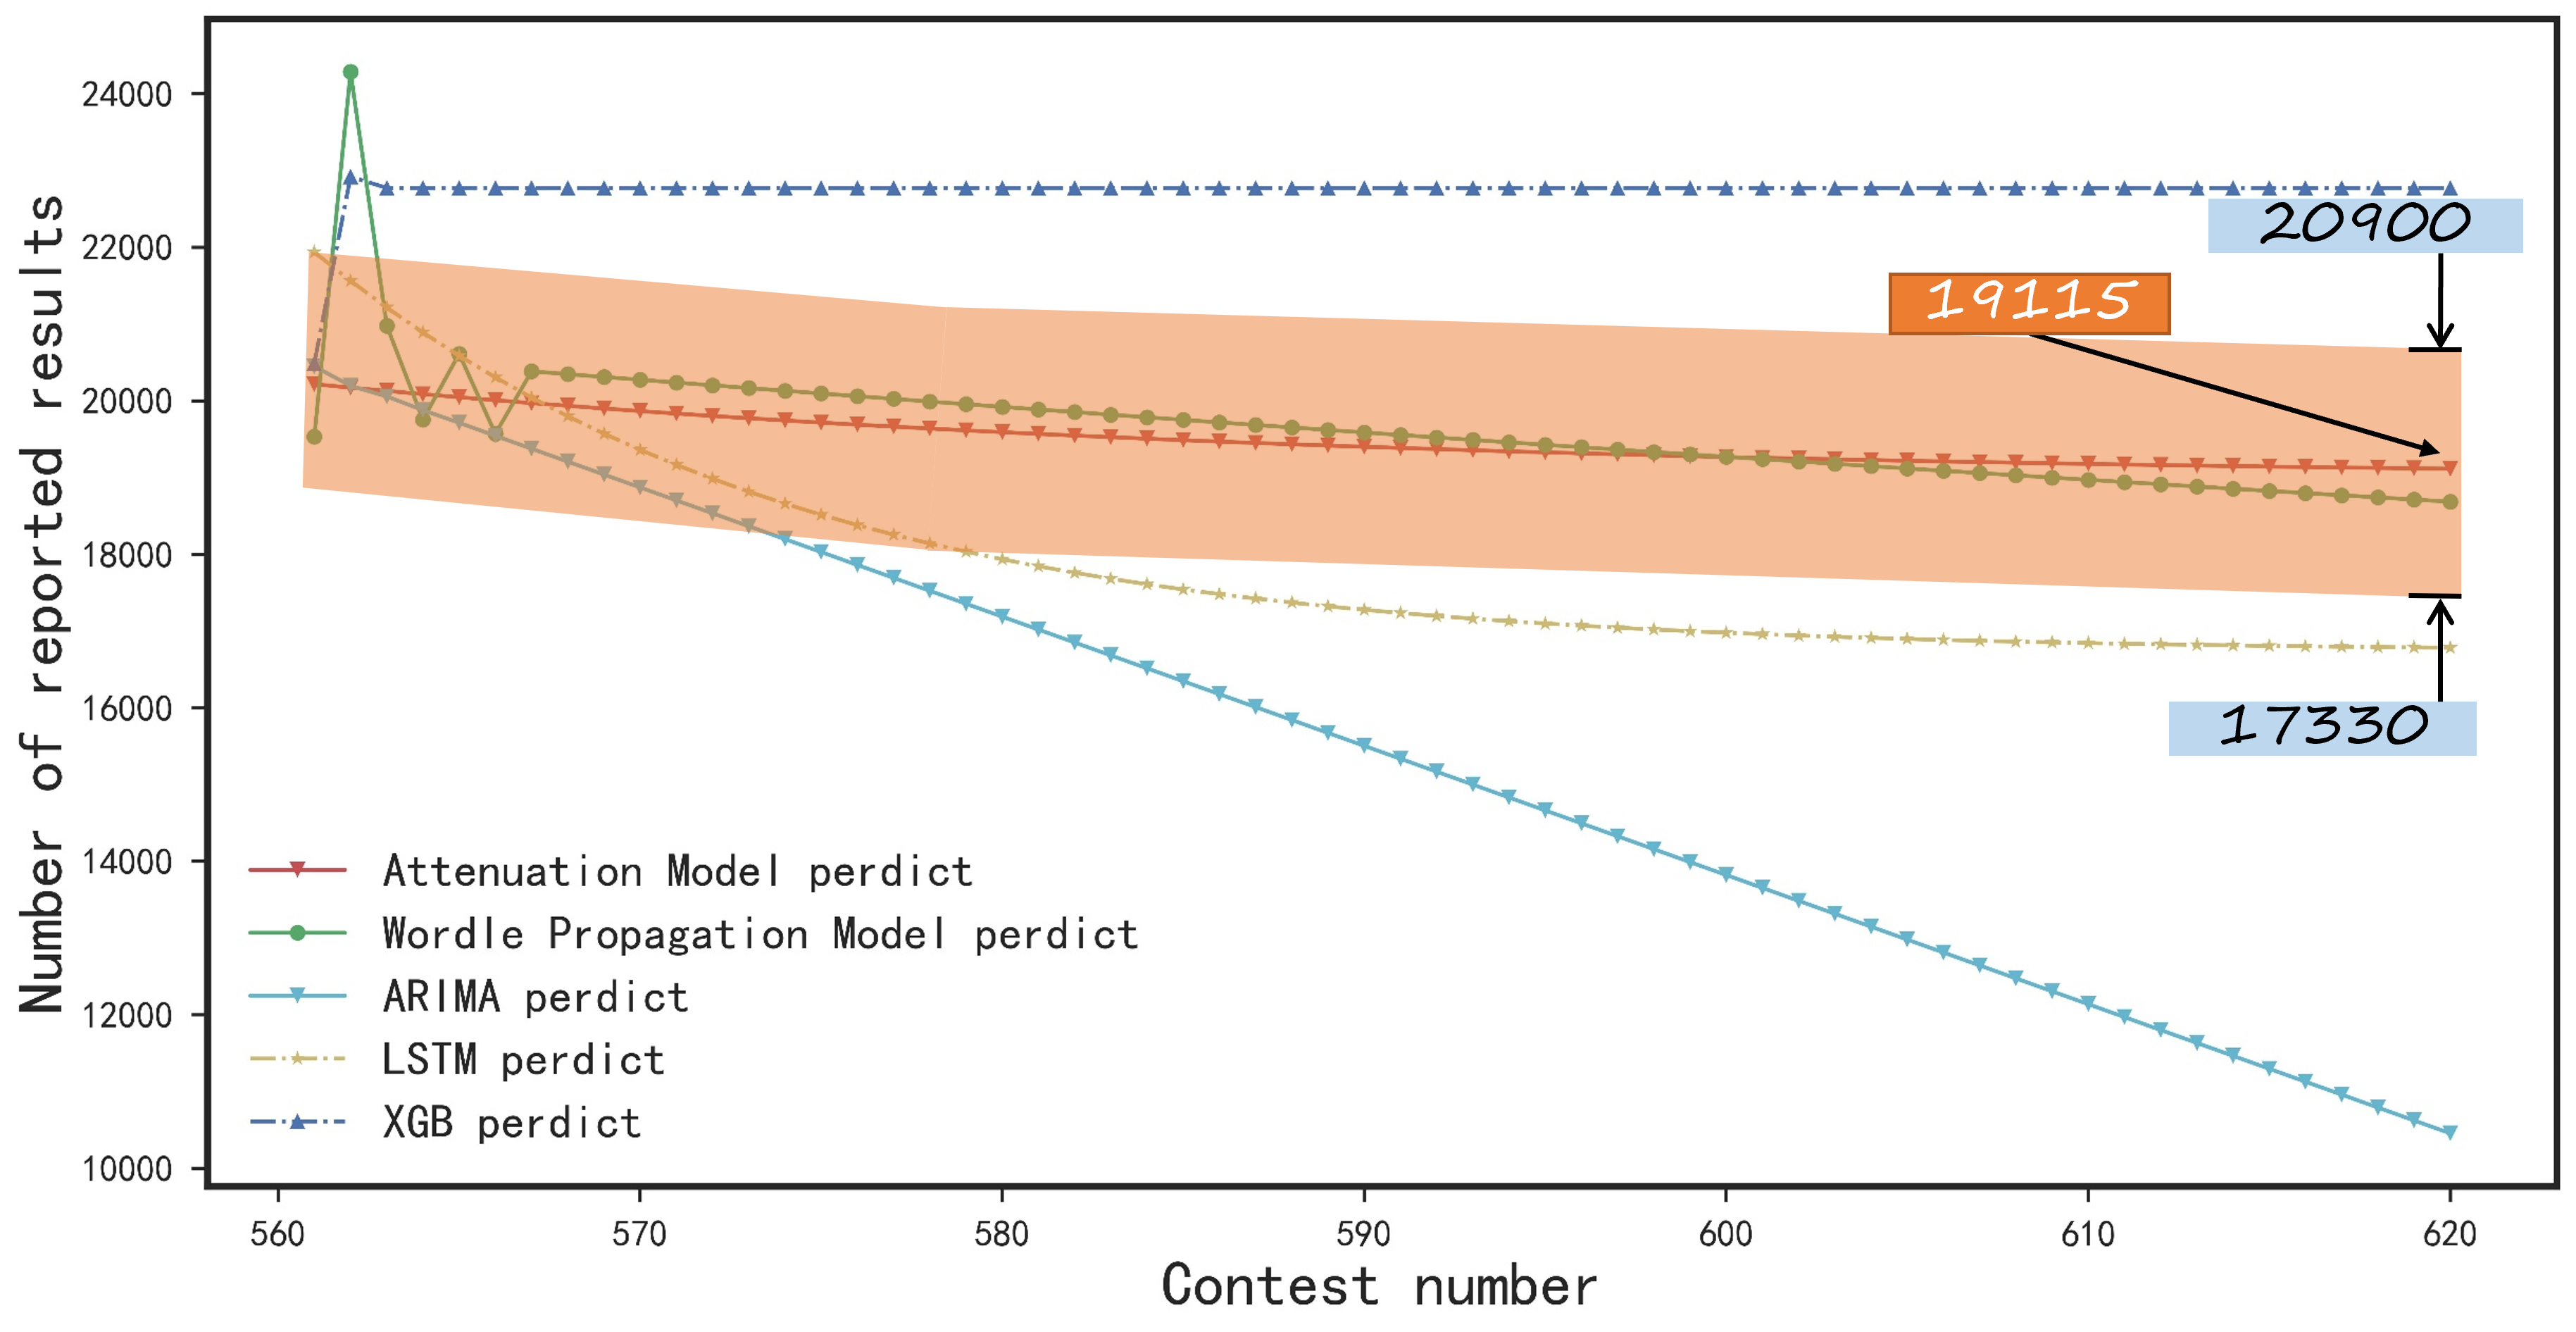
\includegraphics[width=.7\textwidth]{picture1.png}
	\caption{\small The models' predictions for the future}
\end{figure}

By observing the figure, it is found that the original data does not conform to a stable time series, its mean does not have a stable amplitude on the time axis, and its variance does not tend to a stable value. Therefore, there is a big difference between the prediction results of ARIMA and other prediction models of deep learning. However, the Wordle information propagation model based on the complex network propagation dynamics tends to be stable and accords with the expected results.

\subsection{Word feature}
In Wordle games, the factors that affect the guessing times of players include the complexity of word structure, the frequency of word use, the part of speech of the word and other related factors. In order to distinguish the effect of different words on the difficulty of guessing games, we quantified words by analyzing the following attributes.

\subsubsection{Intuitive features}
\begin{itemize}
\item \textbf{Letter combinations} According to word formation, there are some common roots and affixes in English.We split the word and count the frequency of each letter combination, considering that the player may substitute his own vocabulary in the process of guessing the word,It is found that there will be some degree of influence on the percentage of scores reported that were played in Hard Mode.
\item \textbf{Repeat letters} According to the rules of the game, the program doesn't tell the player how many letters they guessed during each guess. So when there are duplicate letters, the difficulty increases. At the same time, this paper defines Classification variable, which can be divided into 1, 2 and 3, among which:

\qquad 1: There are no repeated letters in the word.

\qquad 2: There is only one recurring letter in the word.

\qquad 3: The word has two or more repeated letters.

\qquad Below is a violin diagram of the difficulty for different Classification. You can see that the difficulty increases as the degree of letter repetition increases.
\end{itemize}
%\begin{figure}[H]
%	\centering
%	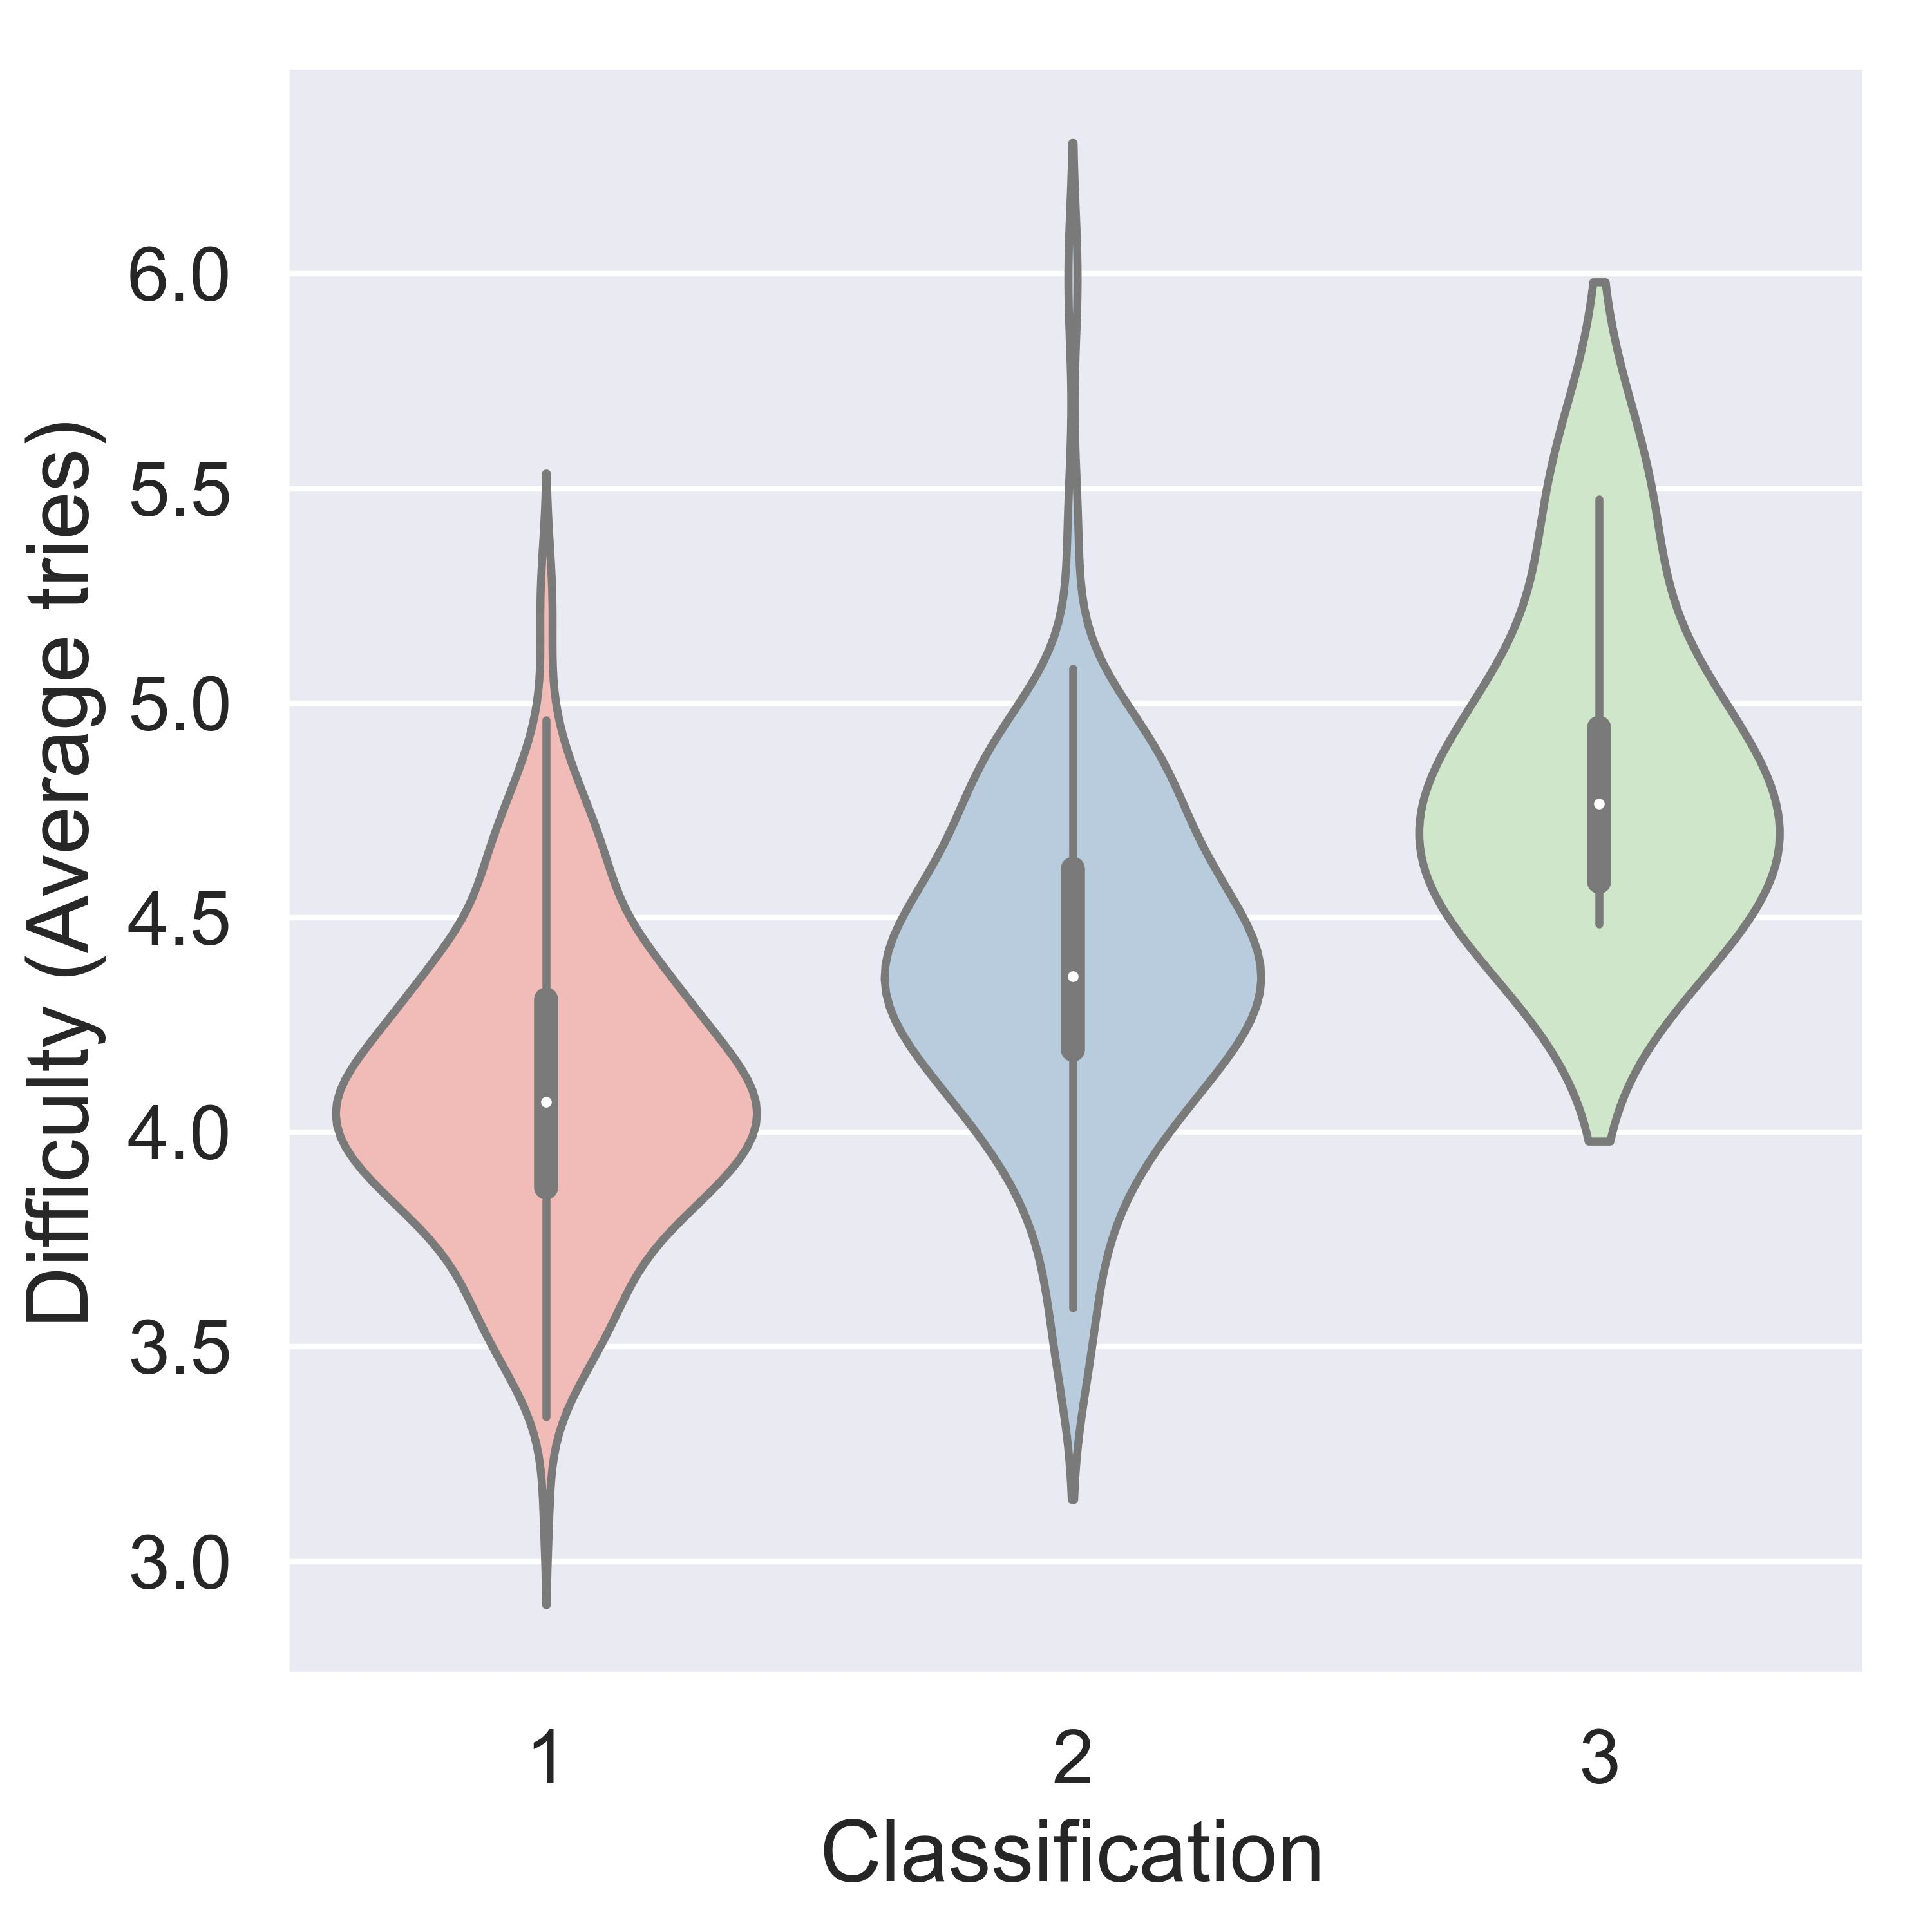
\includegraphics[width=.35\textwidth]{Word_Classification.jpg}
%	\caption{\small Repeat letter classification difficulty}
%\end{figure}
\subsubsection{Hidden Features}
\begin{itemize}
	\item \textbf{Word frequency} The frequency with which a letter appears in text. Wordle's mechanic is to guess and eliminate letters step by step to determine the final answer, so how often letters are used affects the game's problem-solving process. We collected all 5-word words and calculated the frequency with which each letter was used, and found that the higher the frequency of the word, the greater the percentage of scores reported that were played in Hard Mode.
	
	\item \textbf{Word popularity} The total number of 5-word words is about 13,000, compared to just over 2,000 common 5-word words. When playing games, the average player is more likely to guess common words. We obtained the popularity of each word through the Mathmetica program interface and normalized the data using the sigmoid function. Found that low popularity of the answer to the riddle increased the difficulty of the game.
\end{itemize}
%\textbf{1:Word frequency}
%
%Word frequency, the frequency with which a letter appears in text. Wordle's mechanic is to guess and eliminate letters step by step to determine the final answer, so the frequency of letters used definitely affects the game's problem-solving process.
%
%We collected all five words and calculated the frequency of each letter. Here are the five most common letters:
%\begin{table}[H]
%	\centering
%	\caption{\small Letter Frequency}
%	\renewcommand\arraystretch{1.2}
%	\begin{tabular}{cc}
%		\toprule[1.5pt]
%		\makebox[0.25\textwidth][c]{Letter} & \makebox[0.25\textwidth][c]{Freqs} \\
%		\midrule[1.5pt]
%		e & 10.2771559 \\
%		s & 10.2678916 \\
%		a & 9.2441905 \\
%		o & 6.8385702 \\
%		r & 6.4170462 \\
%		\bottomrule[1.3pt]
%	\end{tabular}
%\end{table}
%
%\textbf{2:Groups of letter}
%
%According to word formation, there are some common roots and affixes in English.Considering the players in the process of word guessing may plug in their own accumulation of vocabulary.We split the words and count the frequency of each letter combination. The highest frequencies are listed below:
%\begin{table}[H]
%	\centering
%	\renewcommand\arraystretch{1.2}
%	\caption{\small Word Root Frequency}
%	\begin{tabular}{ccc}
%		\toprule[1.5pt]
%		\makebox[0.23\textwidth][c]{Word Root} &
%		\makebox[0.23\textwidth][c]{Freqs} \\
%		\midrule[1.5pt]
%		es & 1.6675674 \\
%		er & 1.4764919 \\
%		ar & 1.2699761 \\
%		re & 1.2448854 \\
%		ed & 1.2371651 \\
%		\multicolumn{2}{c}{\large ......} \\
%		\bottomrule[1.5pt]
%	\end{tabular}
%\end{table}
%
%\textbf{3:Letter repetition}
%
%According to the rules of the game, the program does not tell the player how many letters they have guessed during each guess. So when there are duplicate letters, the number of letters that can be eliminated by trying is smaller, and the difficulty is relatively higher.
%
%Classification variable is artificially defined, which can be divided into 1, 2 and 3, among which:
%
%1:There are no repeated letters in the word.
%
%2:There is only one recurring letter in the word.
%
%3:The word has two or more repeated letters.
%
%Below is a violin diagram of the difficulty for different Classification. You can see that the difficulty increases as the degree of letter repetition increases.
%\begin{figure}[H]
%	\centering
%	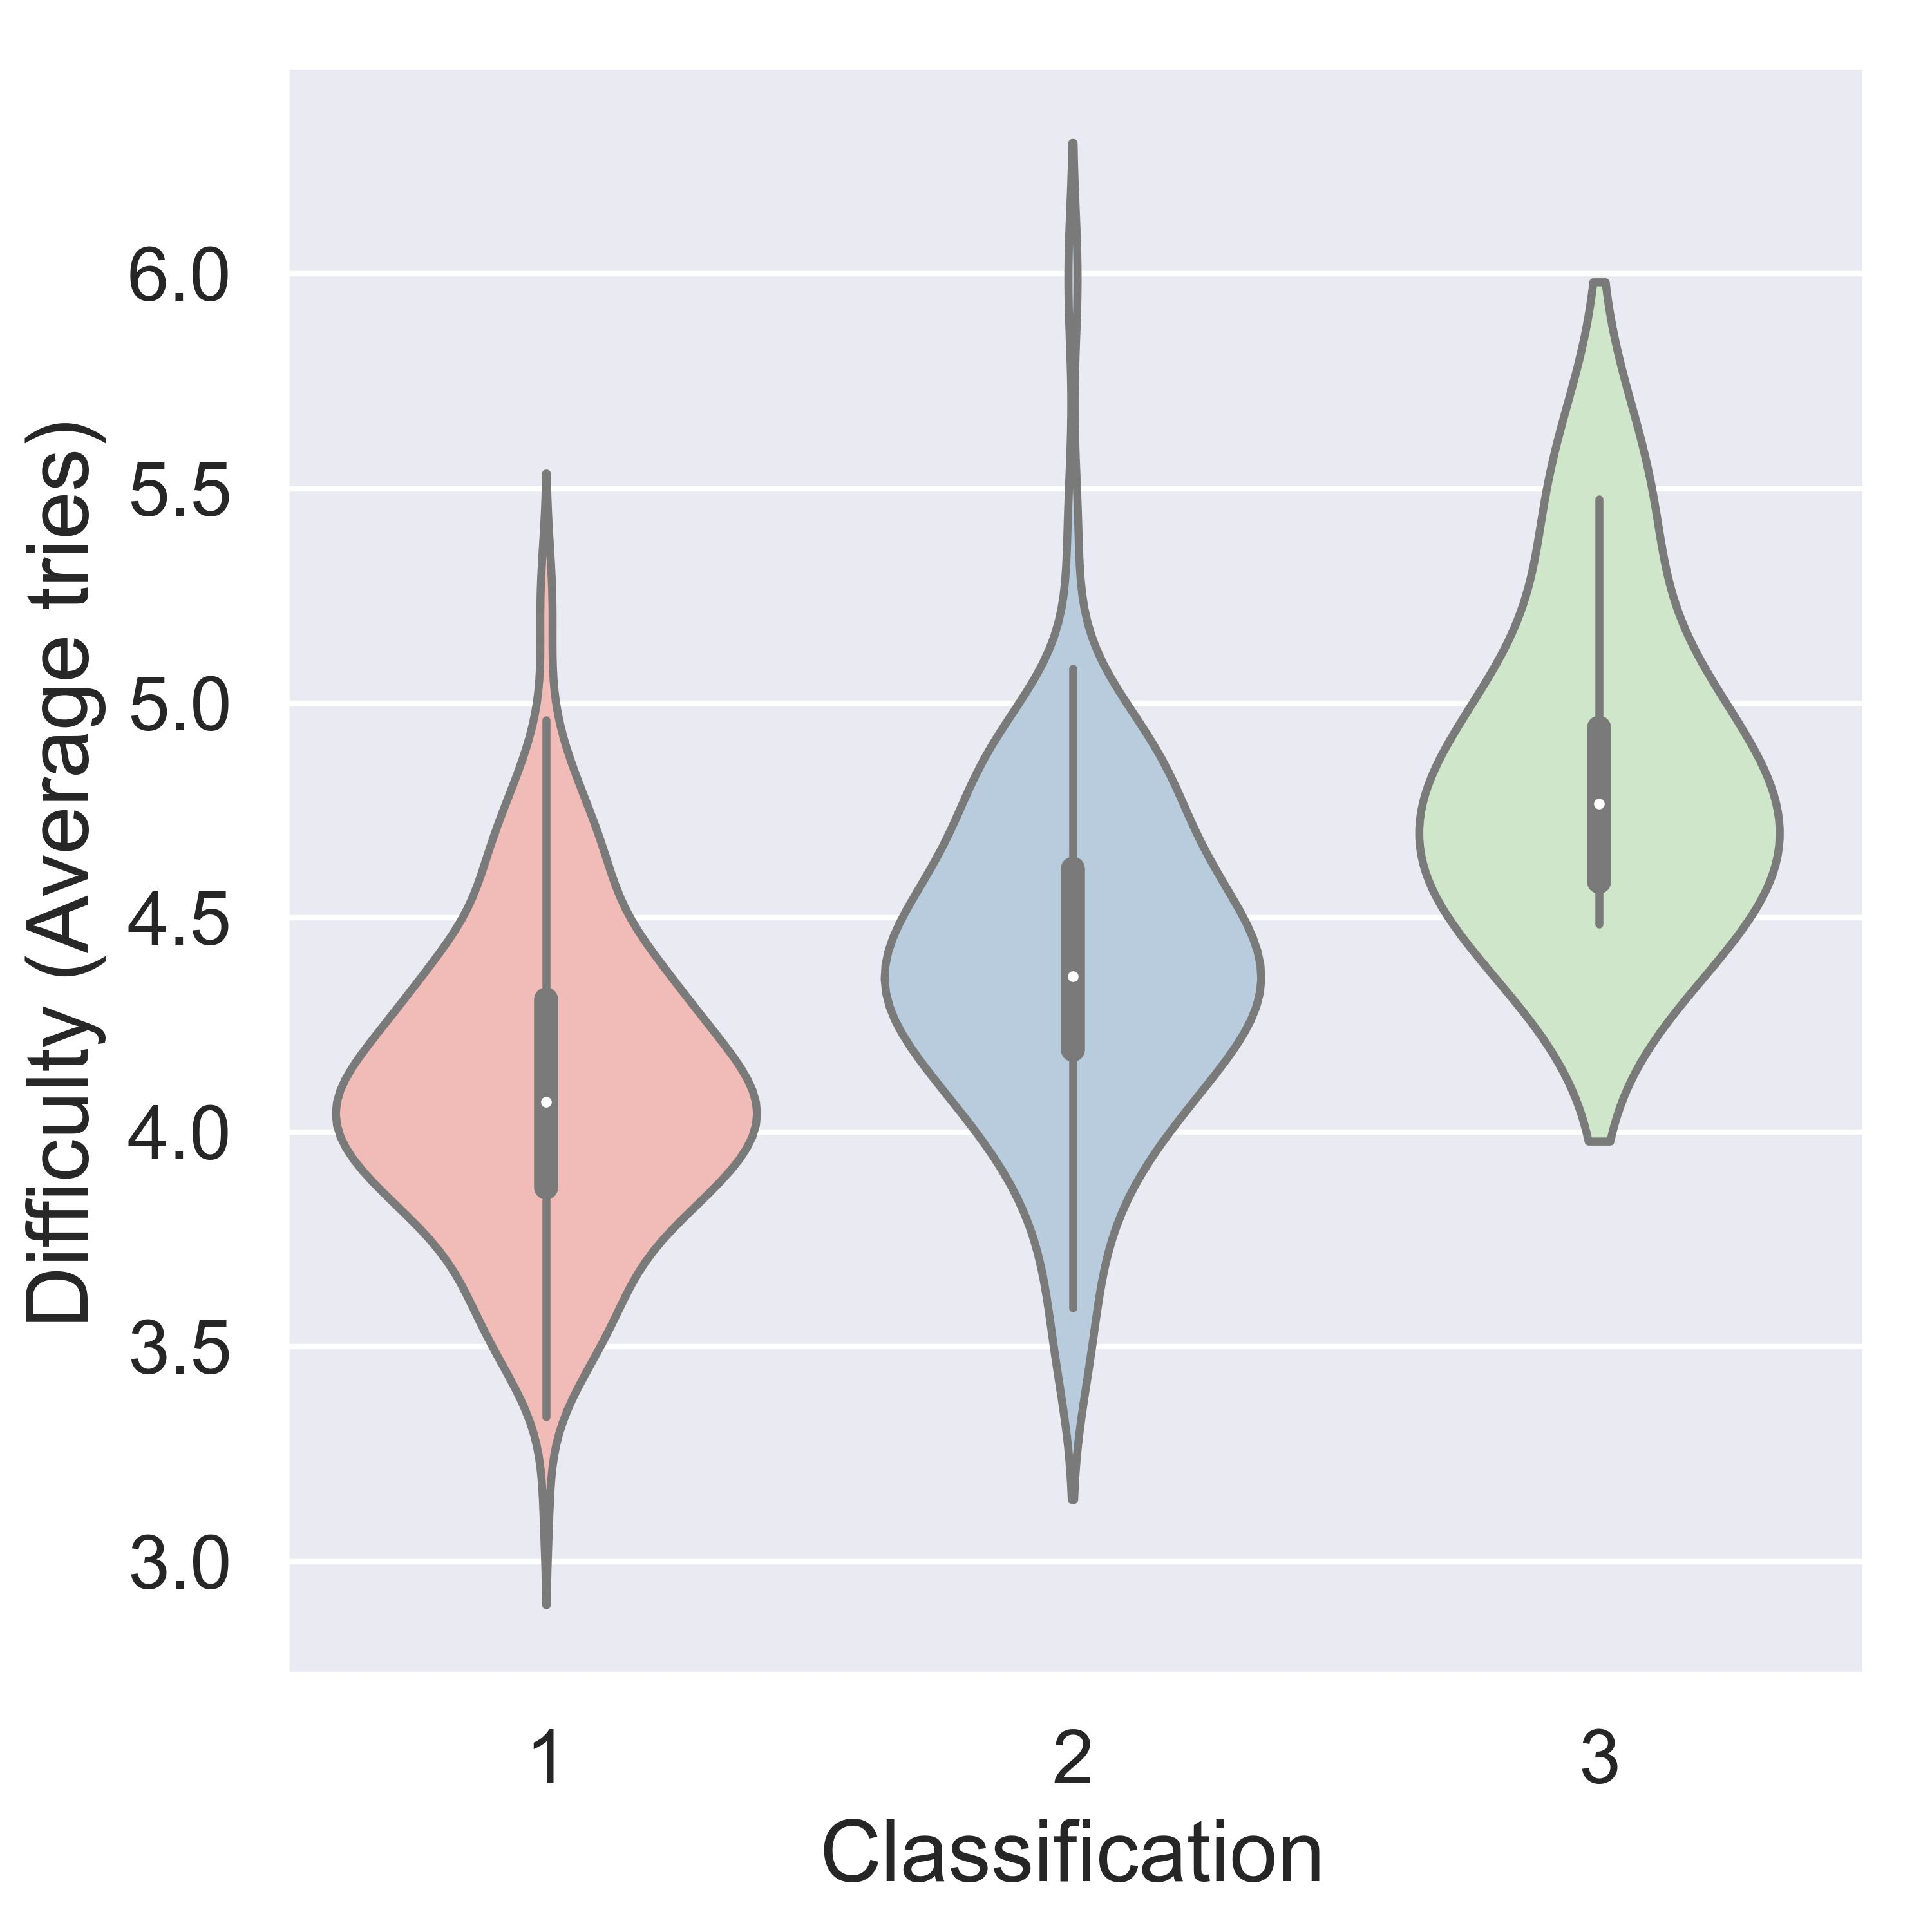
\includegraphics[width=.5\textwidth]{Word_Classification.jpg}
%\end{figure}
\subsubsection{Information entropy}
Charades are about eliminating letters to get to the final answer. And because the letters don't have the same frequency, they don't carry the same amount of information. So we introduce the concept of information entropy to quantize the information of each word.

Take the letter 'e' for example, its word frequency is the highest, so the number of words formed by 'e' is the largest, the uncertainty is the highest, and the information content of 'e' is the largest.

%For the calculation of the amount of information, we lay emphasis on expressing the uncertainty of the event. Information entropy is a measure of how much uncertainty a piece of information can eliminate.
The following is the flow chart of information entropy evaluation:
\begin{figure}[H]
	\centering
	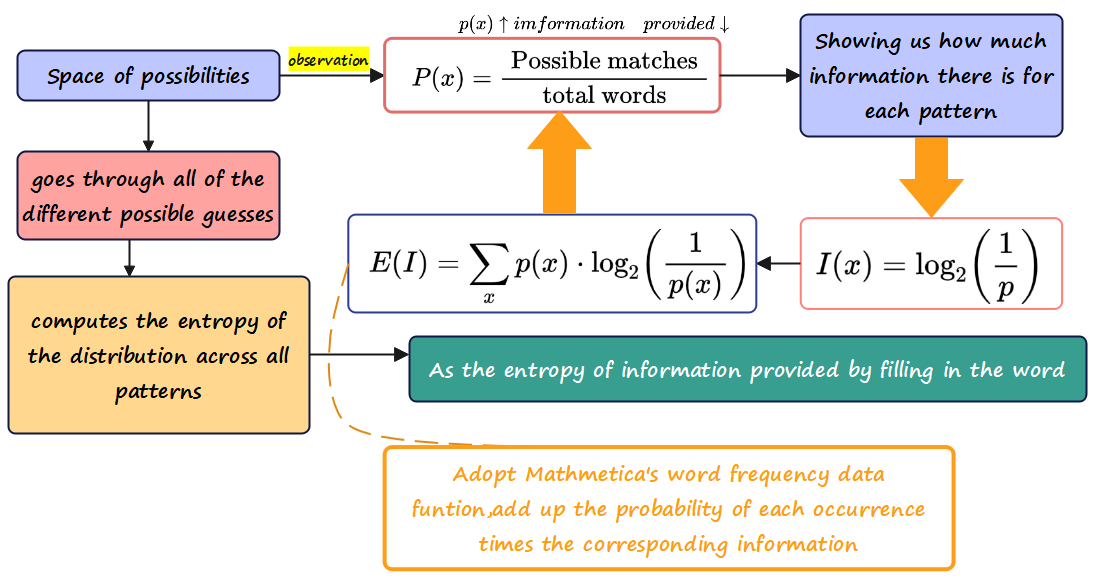
\includegraphics[width=.7\textwidth]{Q1_lct3.png}
	\caption{\small Word information entropy calculation process}
\end{figure}

Because of a meaningful word, there are combinations of letters in a particular order. For example, combinations of 'es' and 'er' are more common than combinations of 'rc' and 'fy'. Therefore in combination with context, the appearance of a letter is not independent, the letter S in the possibility of $P (S) = P (x_n | x_1, x_2,... x_n- 1)$. Since there are too many possibilities, we follow the Markov hypothesis - the probability of any word $w_i$ is only related to the word $x_{i-1}$ before it, and the probability of S is $\mathrm{P}(\mathrm{S})=\mathrm{P}(\mathrm{x} 1) \mathrm{P}(\mathrm{x} 2 \mid \mathrm{x} 1) \mathrm{P}(\mathrm{x} 3 \mid \mathrm{x} 2) \ldots \mathrm{P}(\mathrm{xi} \mid \mathrm{xi}-1)$

According to Markov hypothesis, we build a dual language model:
\begin{eqnarray}
	E(I)  =  -\sum_{x} p\left(x_{n} \mid x_{n-1}\right) \cdot \log _{2} p\left(x_{n} \mid x_{n-1}\right)
\end{eqnarray}
The binary model takes into account the context and word formation, which is more in line with human spelling habits.

Linear regression was performed using information entropy and percentage of attempts. It is obvious that the fourth time is the watershed between information entropy and the percentage of attempts. When the number of attempts is less than 4, the information entropy is proportional to the percentage. This means that the greater the entropy of information, the greater the number of words contained, the greater the proportion of correct attempts in the first three attempts. When the number of attempts is greater than 4, the information entropy is inversely proportional to the percentage. This indicates that the scope of determined words is narrowed, and the smaller the information entropy is, the more correct the word can be determined.
\begin{figure*}[htbp] %通栏
	\begin{minipage}[t]{0.33\linewidth} %调节两个子图左右间距
		\centering
		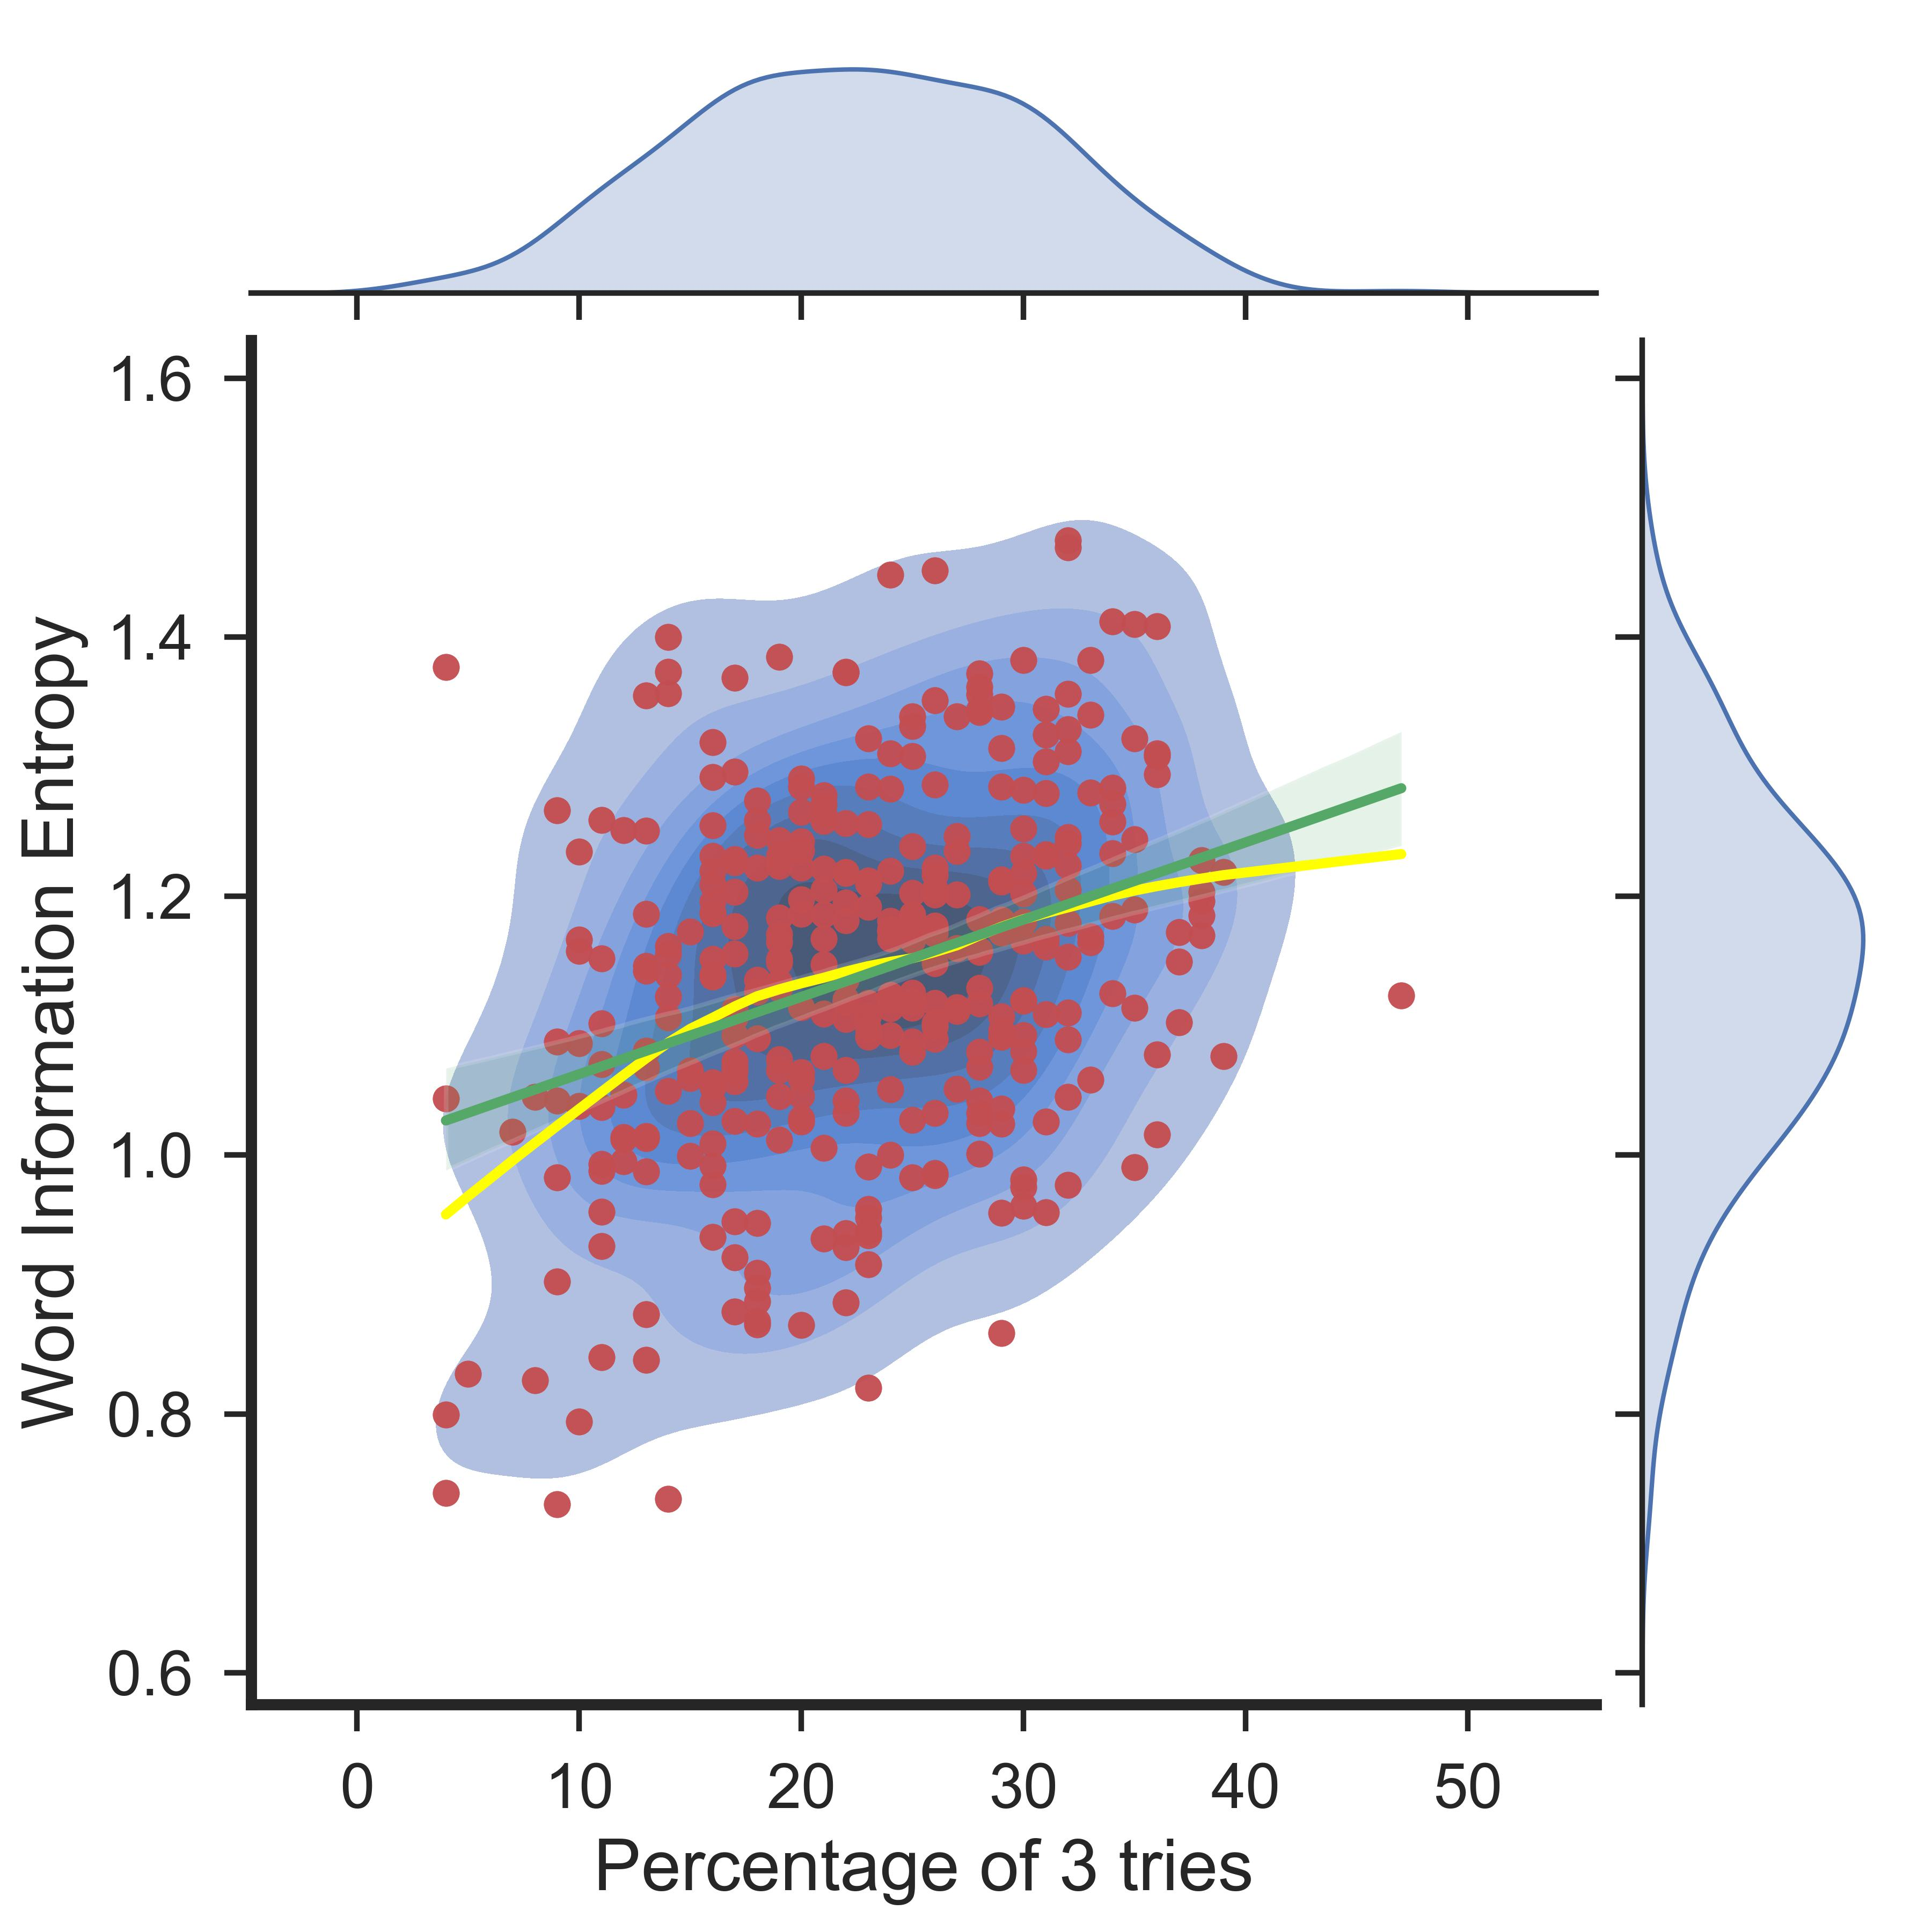
\includegraphics[width=1.9in, height=1.9in]{Word_Information_Entropy_3_tries.jpg} %调节单个子图大小
		\label{fig1} %引用标签
	\end{minipage}%
	\begin{minipage}[t]{0.33\linewidth}
		\centering
		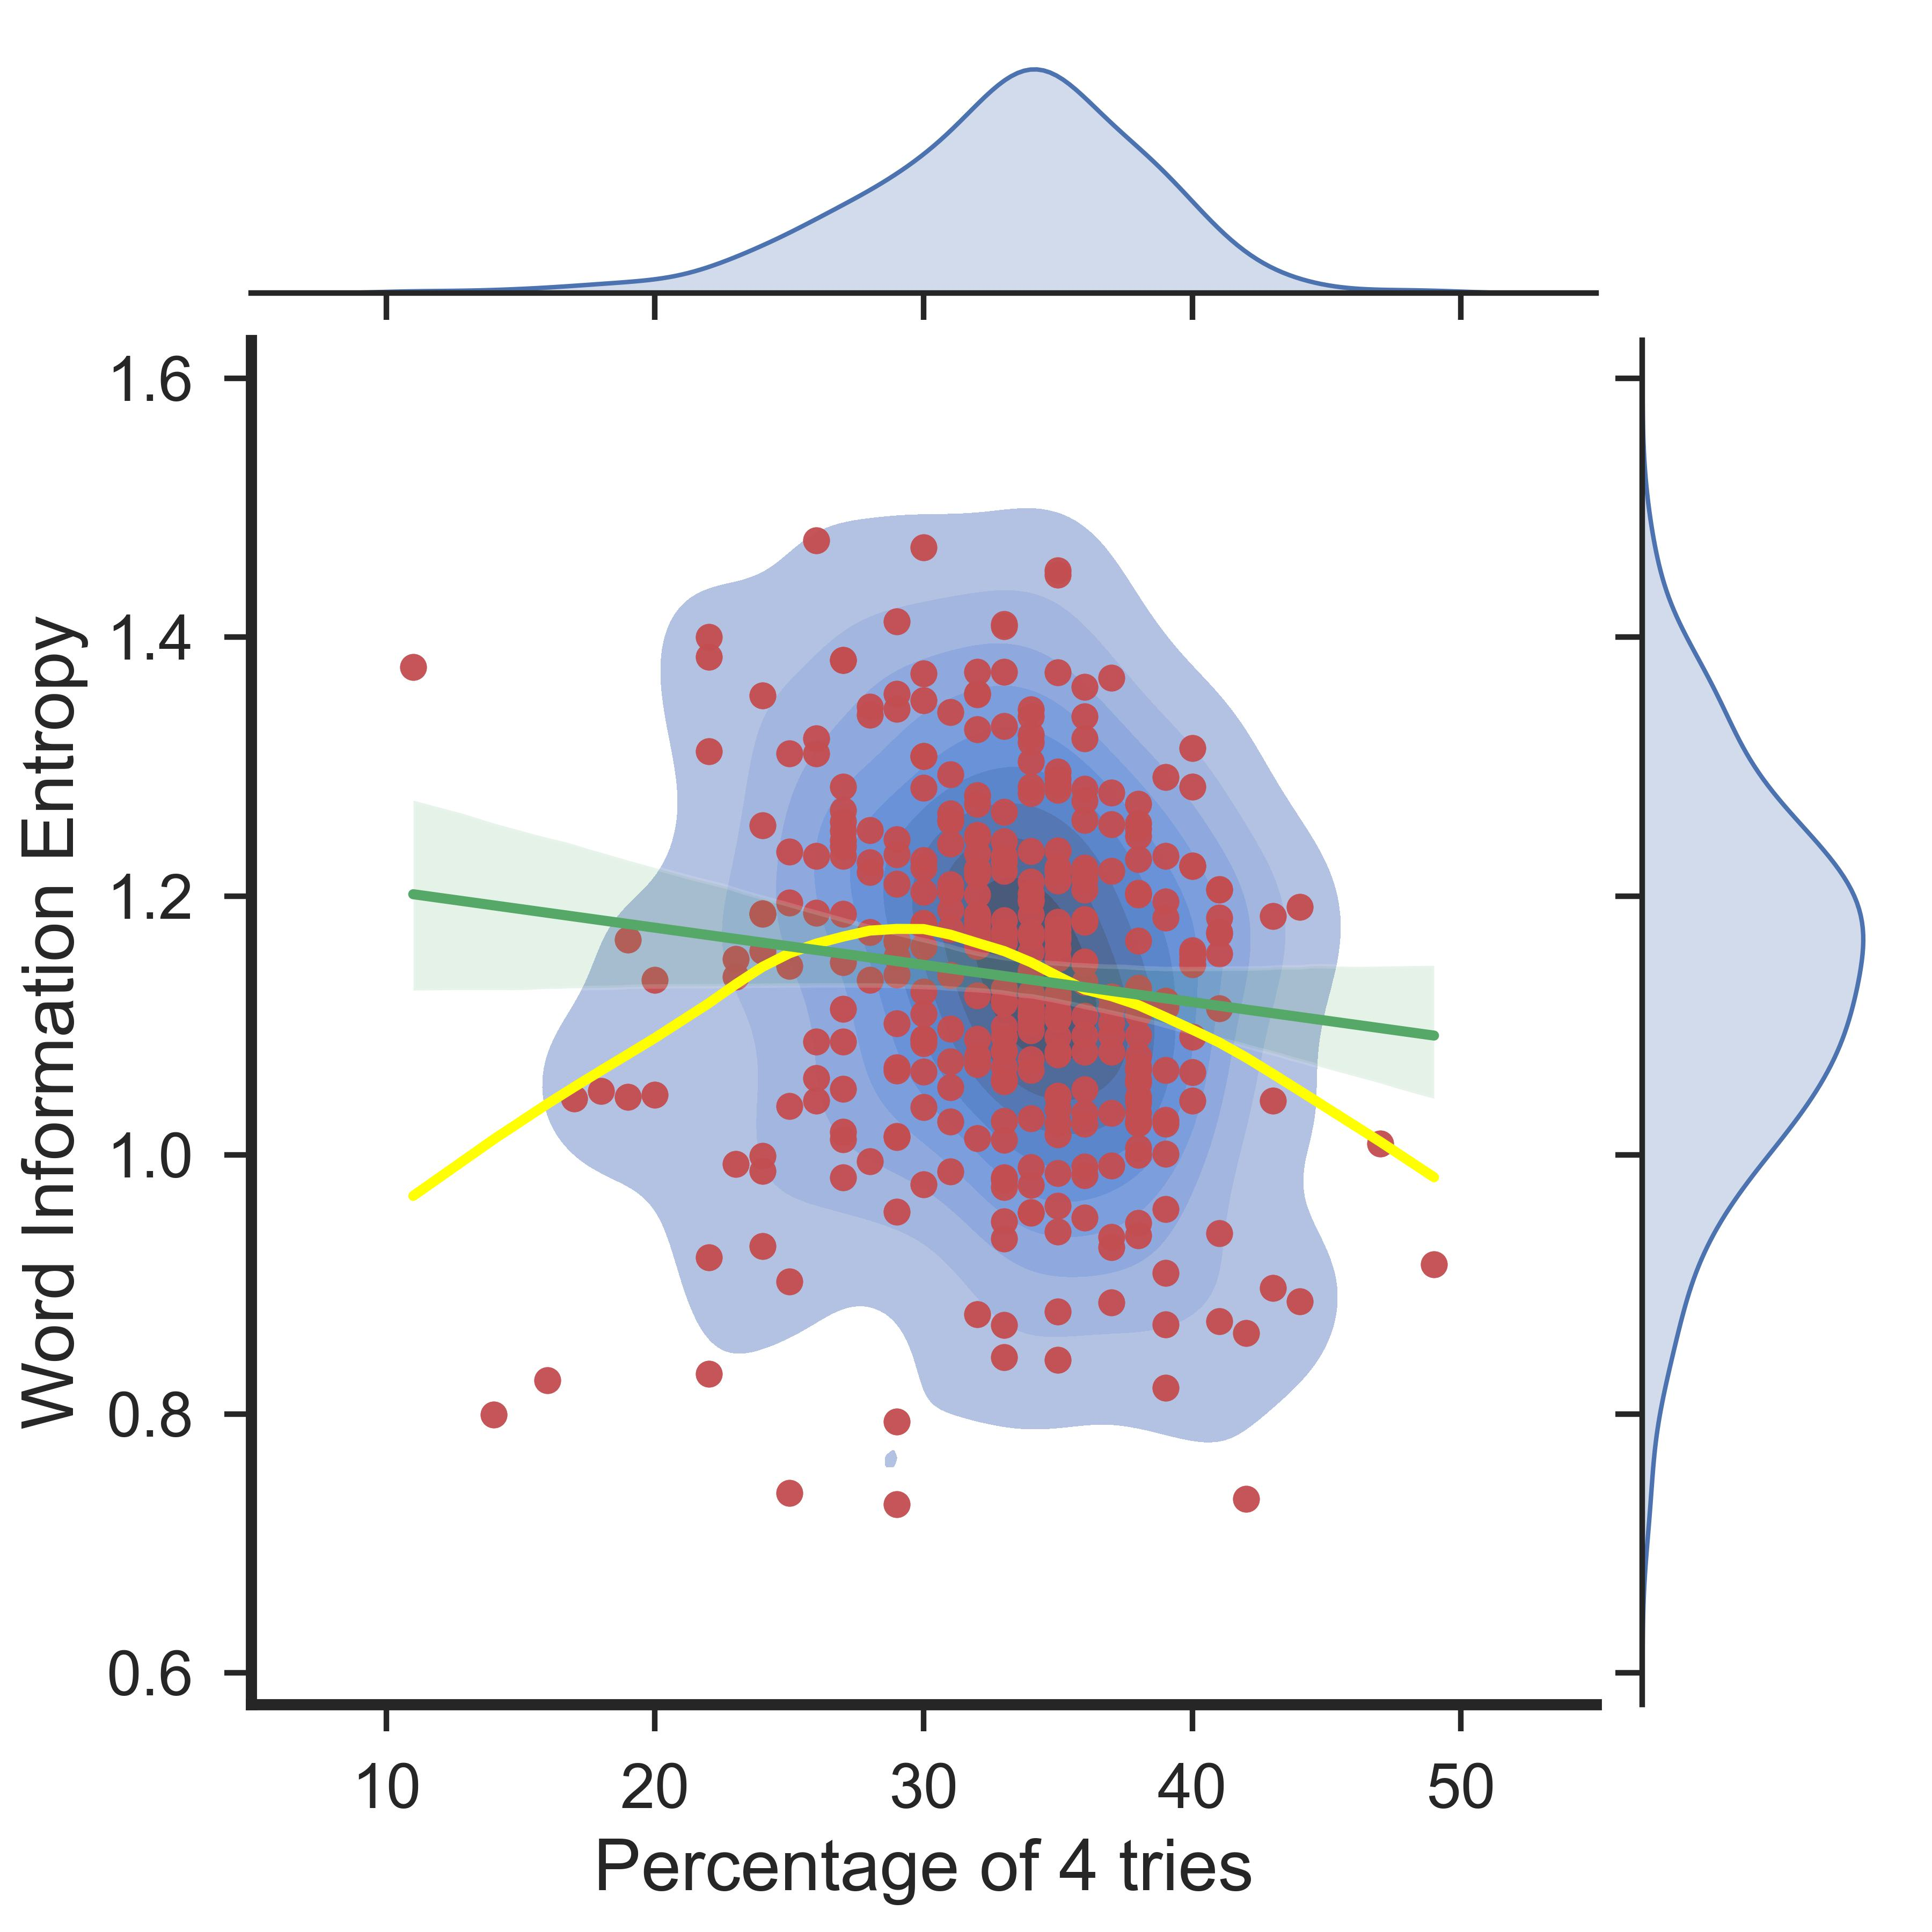
\includegraphics[width=1.9in, height=1.9in]{Word_Information_Entropy_4_tries.jpg}
		\label{fig2}
	\end{minipage}%
	\begin{minipage}[t]{0.33\linewidth}
		\centering
		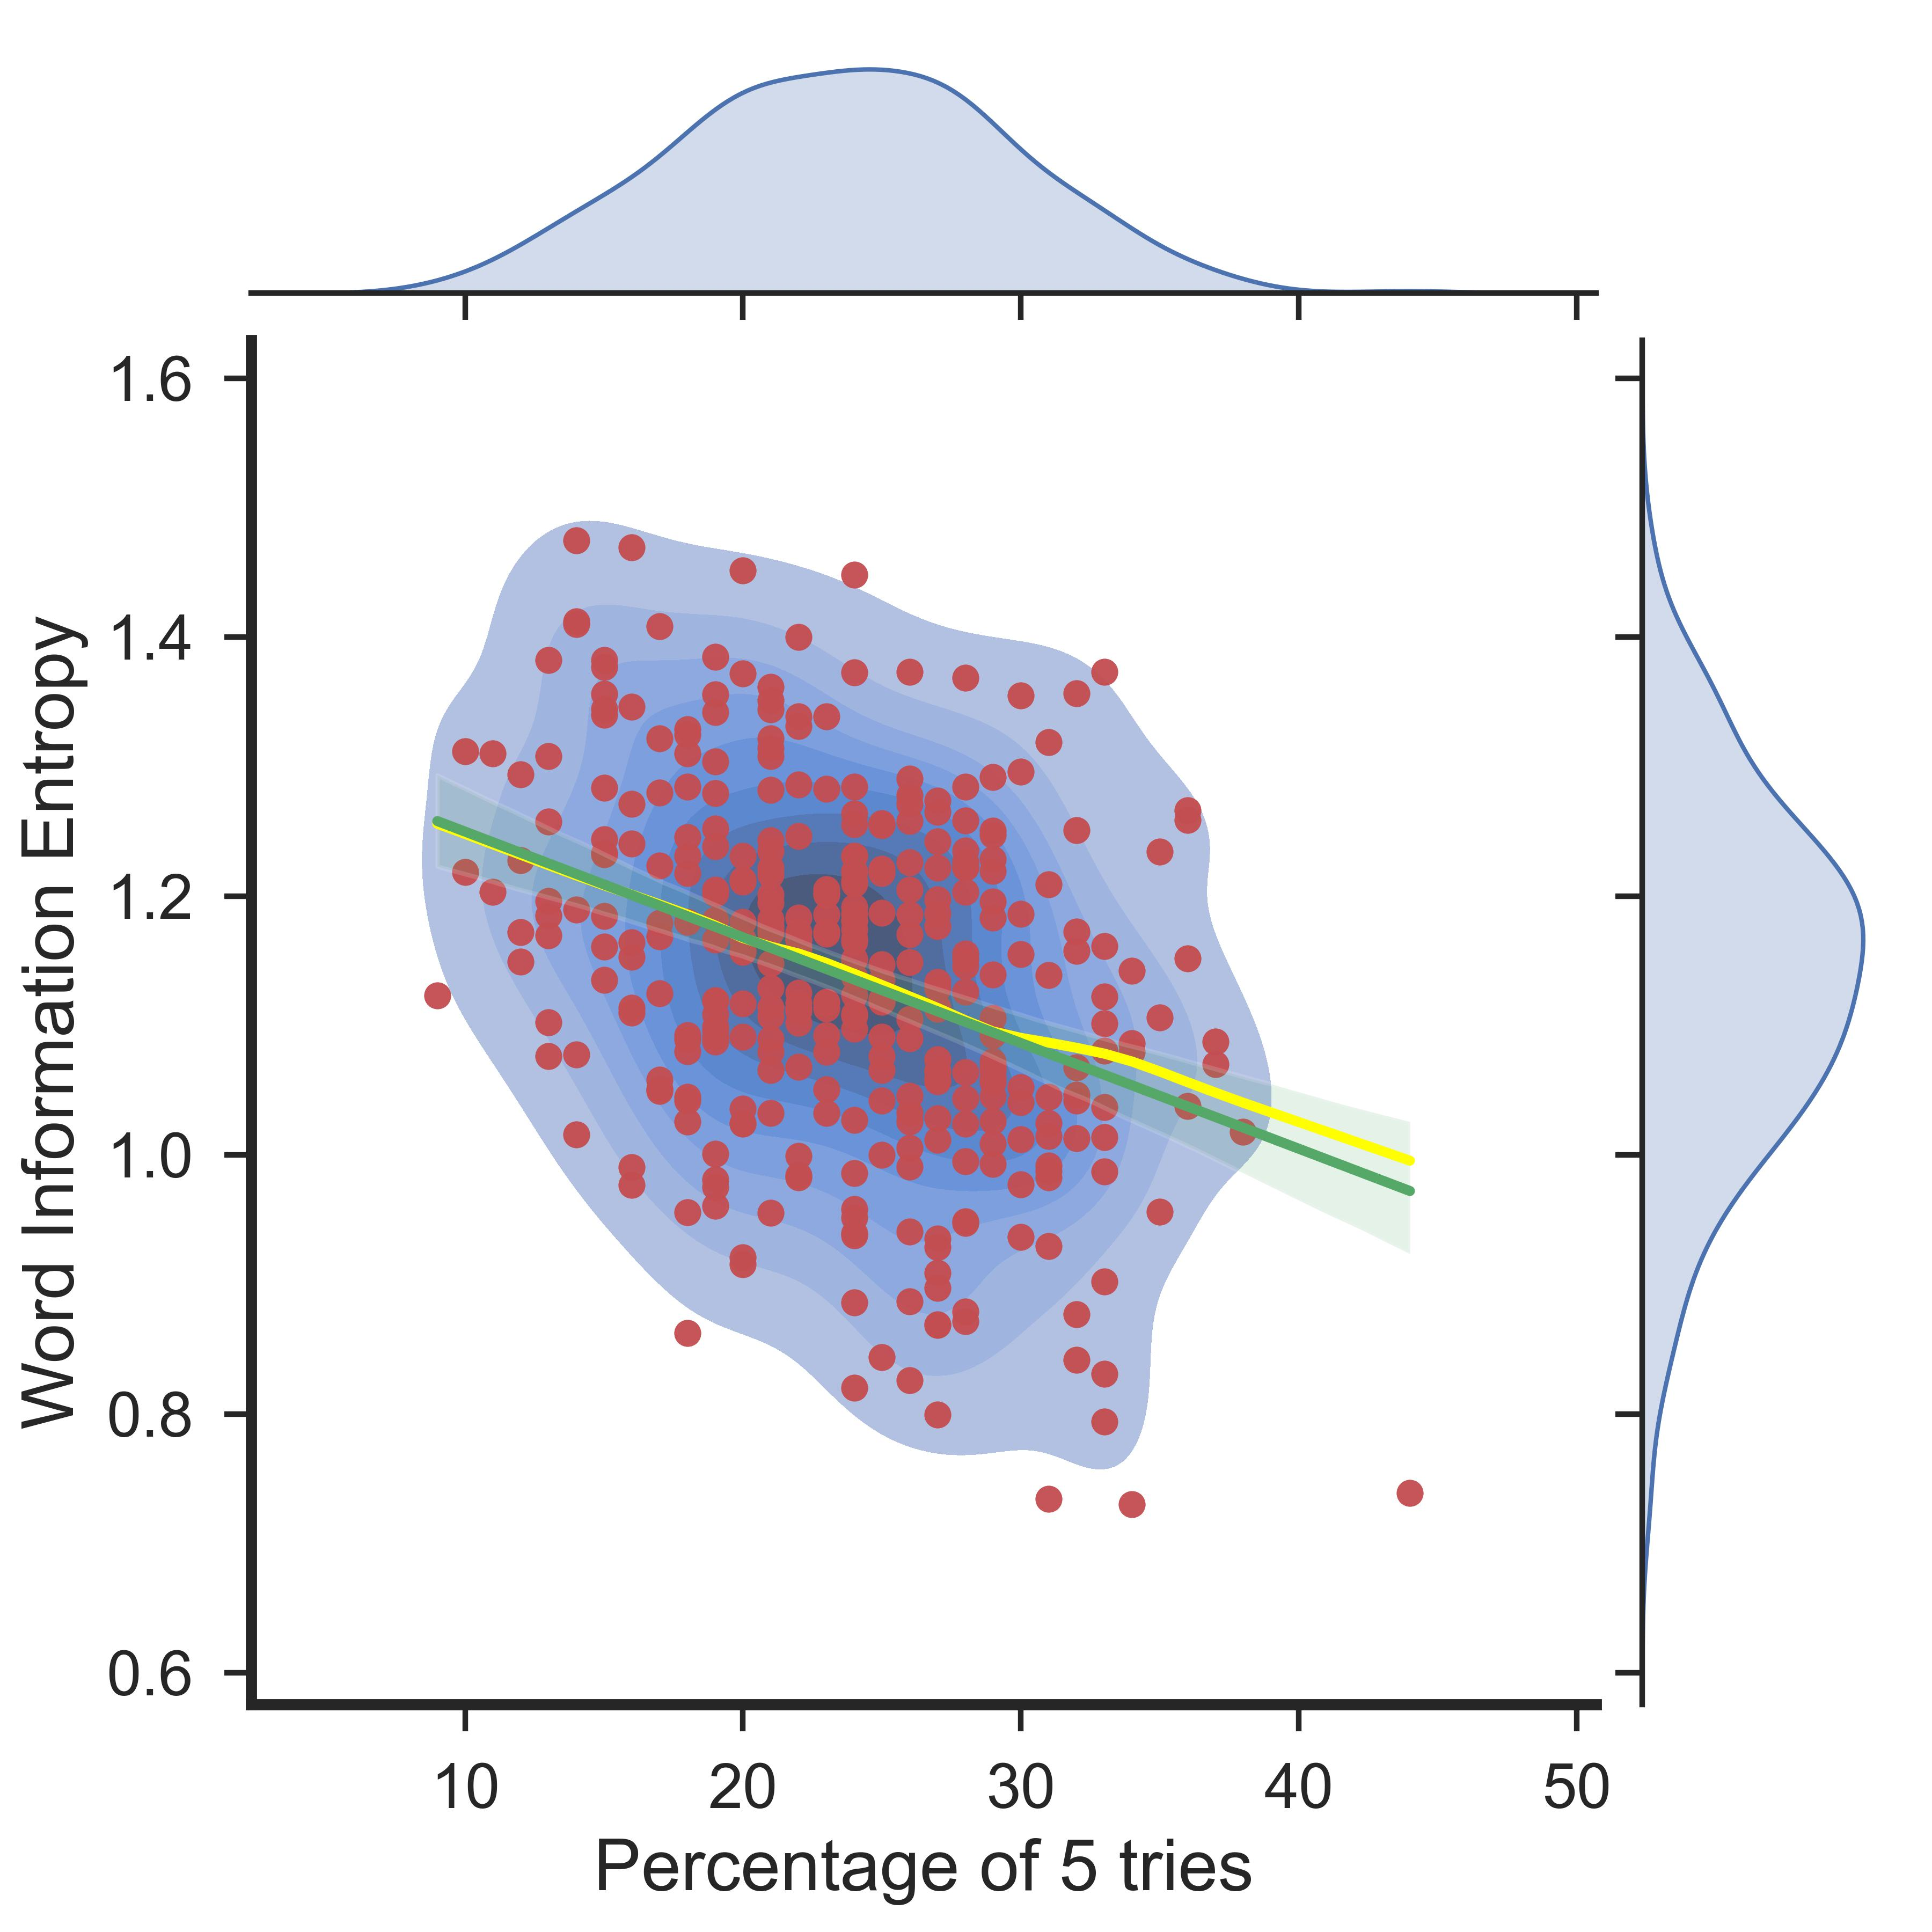
\includegraphics[width=1.9in, height=1.9in]{Word_Information_Entropy_5_tries.jpg}
		\label{fig3}
	\end{minipage}
\end{figure*}

%\textbf{5:Word popularity}
%The total number of 5-word words is about 13,000, compared to just over 2,000 commonly used words. Since most people are familiar with unfamiliar words, the average player is more likely to guess common words when playing games. Therefore, if the answer is not popular, it will make the game more difficult.
%
%We obtained the popularity of each word through the Mathmetica program interface. Because of the distance between the data, certain words are popular, but their popularity varies by tens of times. Therefore, in order to narrow this gap, we use sigmoid function to normalize the data.

%Some data are as follows:

\subsection{Correlation analysis between word attribute and number of attempts}

For the above word attributes, Spearman correlation analysis was conducted between them and the percentage of attempts. The heat map is as follows:
\begin{figure}[H]
	\centering
	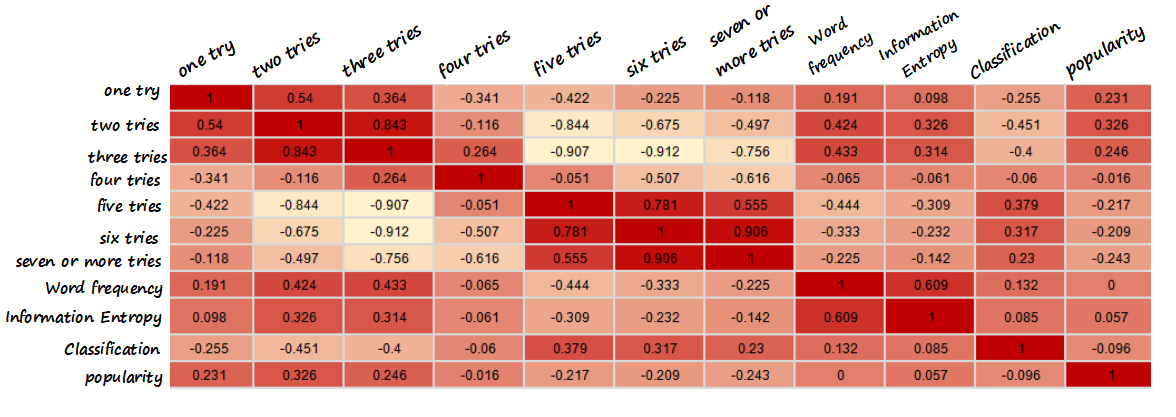
\includegraphics[width=.8\textwidth]{Q1_rlt.png}
	\caption{\small Heat map}
\end{figure}

Word frequency is the harmonic average of the frequency of each letter in the word.
It can be found that Word frequency, Information Entropy and Popularity are significantly positively correlated with the first three attempts, and negatively correlated with the latter several attempts. In conclusion, when the Word frequency, Information Entropy and Popularity of a word increase, players are more likely to guess the word correctly in the first three guesses, and the word is simpler.
Classification is negatively correlated with the first three attempts and positively correlated with the next few attempts. This suggests that the more letters in a word are repeated, the more guesses users need to make, and the more difficult the word is.

\section{Regression prediction on the number of guesses}
\subsection{Stepwise regression model}
For problem two, we classified the percentage of different attempts according to Classification, and carried out visual analysis on the feature data of words.It can be found that the percentage of attempts is related to word frequency, word information entropy, classification of repeated letter number, word popularity, letter number and other factors.
%\begin{figure}[H]
%	\centering
%	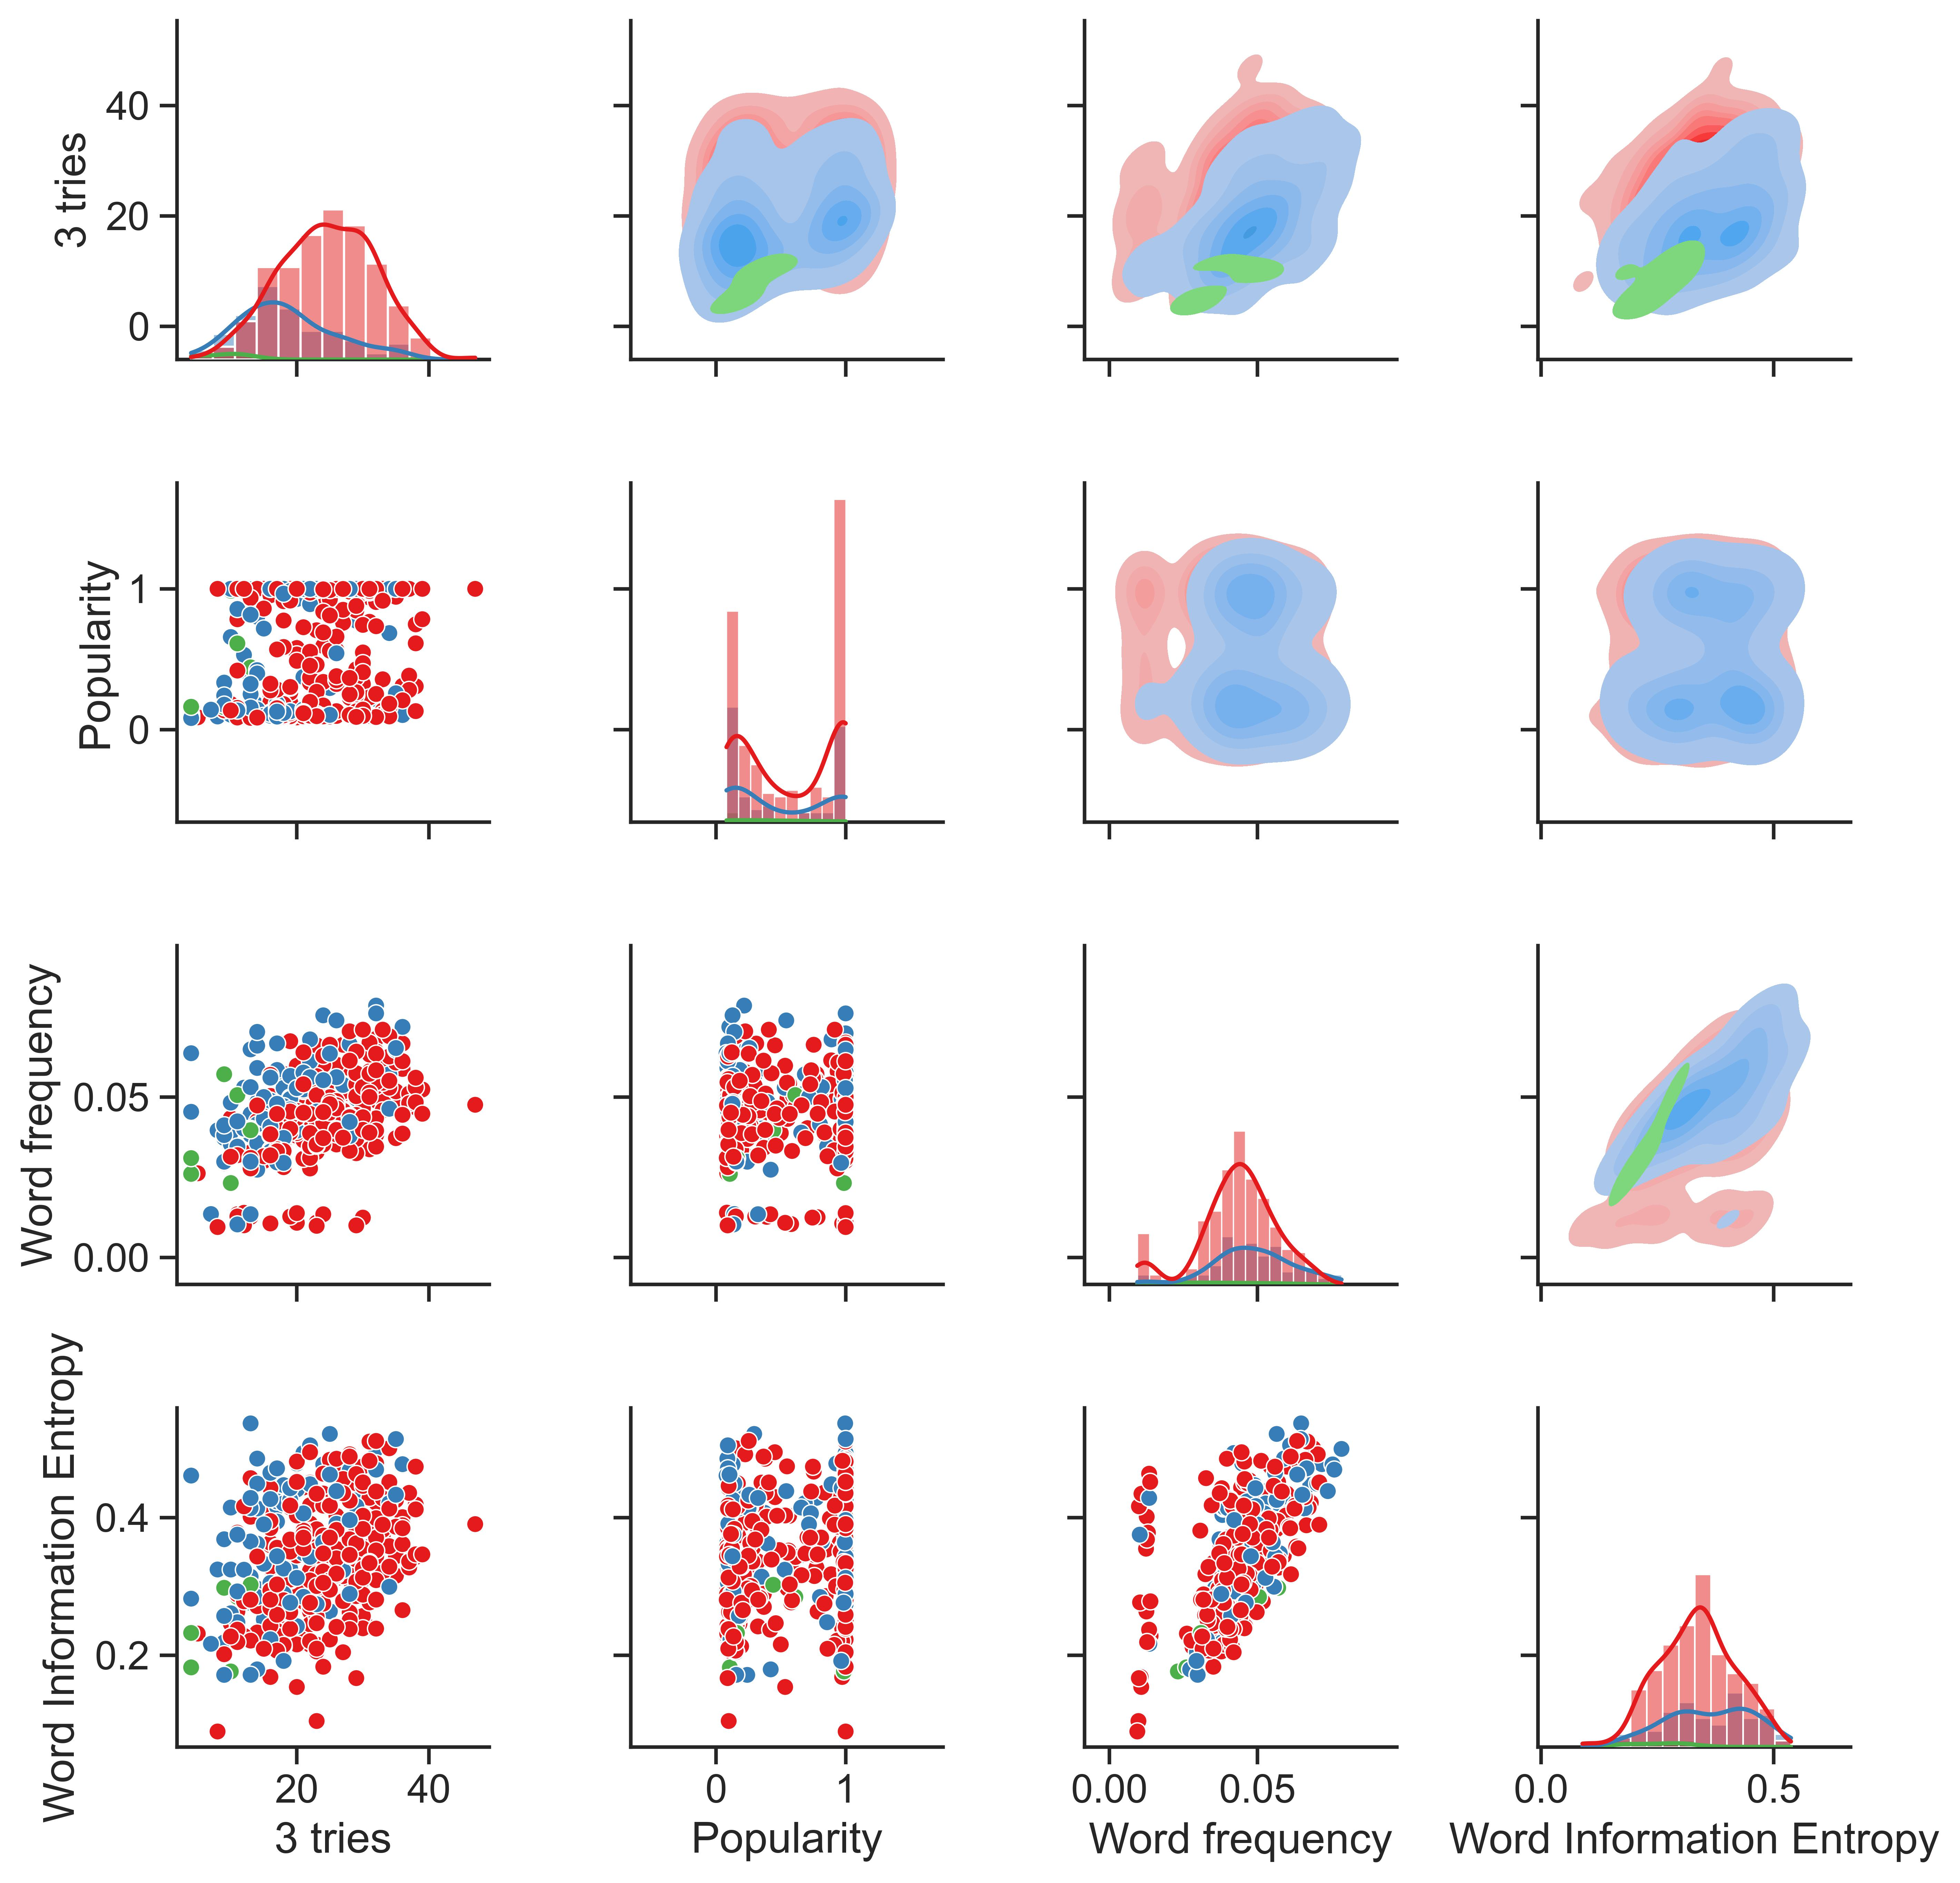
\includegraphics[width=.45\textwidth]{Word_Tries.jpg}
%	\caption{\small 3 tries' Data visualization}
%\end{figure}

In order to avoid multicollinearity problems, multiple stepwise regression method was used for prediction, and mathematical models were established for different percentages of attempt times, such as word frequency, word information entropy, classification of repeated letter number, word popularity, letter number and other factors. After introducing all the independent variables into the model, the independent variables that contributed little to the sum of the squares of the residual parameters and the squares of other parameters were eliminated one by one. After several iterations, no independent variables met the exclusion conditions. In this way, a more accurate multiple linear regression equation is established.\\
\textbf{Dependent variable}
\begin{itemize}
	\item Percentage of each guess (1 try, 2 tries,.... ,7 or more tries (X))
\end{itemize}
\textbf{Argument}
\begin{itemize}
	\item Word frequency ($F$) : The word frequency of the word
	\item Word information entropy ($E$) : The information entropy of the word
	\item Repeated letter classification ($C$) : The word is categorized by the number of repeated letters
	\item Word popularity ($P$) : The popularity of the word
	\item Letter count ($L_i$) : The number of letters appearing in the word, where $i=a,b,...,y,z$
\end{itemize}
\begin{eqnarray}
	\text { Percentage }_i  =  \alpha_{i}+\beta_{i} F_{i}+\gamma_{i} E_{i}+\delta_{i} C_{i}+\varepsilon _{i} p_{i}+\sum \lambda _{i} L_{n}+\mu_{i}
\end{eqnarray}

According to the formula, the percentage of each attempt times was substituted into the data, and finally 7 corresponding multiple regression equations were obtained.All regression equations passed the F-test (joint hypothesis test) and were valid equations.

By constructing stepwise regression model, the prediction equation corresponding to each number of guesses is obtained.See the table below:

\begin{table}[H]
	\centering
	\footnotesize
	\renewcommand\arraystretch{1.12}
	\caption{Stepwise regression equation result table}
	\begin{tabular}{clll}
		\toprule[1.5pt]
		No. of attempts  & Regression equation                                                                                                                                                                                         & F-test      \\ \midrule[1pt]
		$Try_1$           & $y = 0.031+15.436F-0.358C+0.384P$                                                                                                                                             & \begin{tabular}[c]{@{}l@{}}F=20.527\\ P=0.000***\end{tabular} \\
		$Try_2$           & $y = 2.444+123.637F-2.942C+2.258P+1.272L_t-1.245L_y+0.858L_a-0.665L_l$                                                                                                        & \begin{tabular}[c]{@{}l@{}}F=43.161\\ P=0.000***\end{tabular} \\
		$Try_3$           & \begin{tabular}[c]{@{}l@{}}$y=17.592-6.586C+183.392F+3.32P+2.051L_t+2.357L_p+2.22L_h-2.913L_y$\\   $-1.756L_e-2.998L_w+10.036E+1.666L_d+1.36L_i-2.482L_v-1.548L_g$\end{tabular} & \begin{tabular}[c]{@{}l@{}}F=32.081\\ P=0.000***\end{tabular} \\
		$Try_4$           & $y=34.213+2.537L_p-7.611L_z-1.297L_r-1.236L_e-1.151L_a $                                                                                                                      & \begin{tabular}[c]{@{}l@{}}F=8.485\\ P=0.000***\end{tabular}  \\
		$Try_5$           & \begin{tabular}[c]{@{}l@{}}$y=31.75-198.567F+5.047C-2.58L_h-2.475P-1.982L_t-2.08L_p$\\   $-1.741L_c-1.142L_i+1.077L_e-4.448L_q-1.493L_d-7.01E$\end{tabular}                     & \begin{tabular}[c]{@{}l@{}}F=38.512\\ P=0.000***\end{tabular} \\
		$Try_6$           & \begin{tabular}[c]{@{}l@{}}$y=12.054-115.629F+4.28C-2.471P-2.081L_p+2.698L_y$\\   $+1.008L_e-1.573L_t+7.533L_z+2.687L_v+2.141L_w$\end{tabular}                                  & \begin{tabular}[c]{@{}l@{}}F=22.326\\ P=0.000***\end{tabular} \\
		$Try_7 $          & $y=1.724+1.477C-1.509P$                                                                                                                                                       & \begin{tabular}[c]{@{}l@{}}F=10.566\\ P=0.000***\end{tabular} \\
		\bottomrule[1.5pt]
	\end{tabular}
\end{table}

According to the obtained regression analysis table, the regression model was established based on the retained independent variables, and the significance p-values of F-test were all less than 0.01, showing the level of significance. The original hypothesis that all regression coefficients were 0 was rejected, indicating that the model was well constructed.

\subsection{Uncertain factors}
In the prediction process of the model, we take into account the following possible uncertainties:

1.Since the sample data is collected from players voluntarily Posting on Twitter, considering the differences in individual personalities of each player, some players may be inclined to post better results on the social platform, and it is also possible that the word as the answer to the riddle on the same day is more difficult, resulting in more players willing to show the results they are proud of. As a result, the collected data may have some subjective bias, which cannot guarantee the absolute randomness of the sample data.

2.During the prediction process, no relevant metrics were found to distinguish the categories of players. As the game progresses over a longer period of time and the number of older players increases, it is possible that this increase in proficiency will lead to an increase in the average player's ability to guess words, taking into account the growth of the players themselves.

3.At the same time, due to the unpredictability of the word as the answer to the riddle, the word itself may be fermented by some events and appear as a hot word on the Internet, which cannot guarantee the absolute perfection of the model's judgment on the characteristics of the word, which may lead to certain deviation between the predicted results and the actual situation.

\subsection{Prediction of model}
Here are EERIE's indicators and predictions:
\begin{table}[H]
	\centering
	\begin{tabular}{ccccccc}
		\toprule[1.5pt]
		\multicolumn{7}{c}{The Indicators of EERIE} \\  \midrule[1.5pt]
		 \makebox[0.1\textwidth][c]{E} 
		& \makebox[0.1\textwidth][c]{P} & \makebox[0.1\textwidth][c]{F} 
		& \makebox[0.1\textwidth][c]{C} & \makebox[0.1\textwidth][c]{$L_e$} 
		& \makebox[0.1\textwidth][c]{$L_i$} & \makebox[0.1\textwidth][c]{$L_r$}\\
		0.558886 & 0.463777 &	0.080604 &	3 &	3 &	1 &	1    \\  \bottomrule[1.5pt]
	\end{tabular}
\end{table}

\begin{figure}[H]
	\centering
	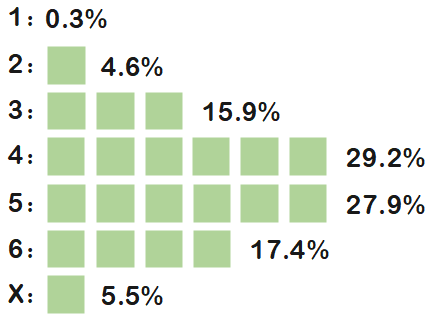
\includegraphics[width=.35\textwidth]{eerie.png}
	\caption{\small The predicted results for EERIE }
\end{figure}

\subsection{Test of the model}
For the test of the model, we calculated the average error of the actual value and the predicted value of the percentage of each attempt (see the figure below). It can be seen that the error is between $\pm 2\%$ , indicating that the model has high accuracy in the percentage of each attempt in the prediction of difficult mode.
\begin{figure}[H]
	\centering
	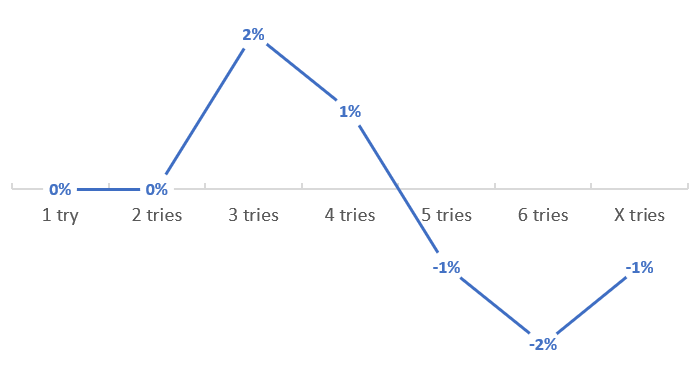
\includegraphics[width=.5\textwidth]{Q2_pjwc.png}
	\caption{\small The average error}
\end{figure}

\section{Classification and evaluation of word difficulty}
\subsection{K-means construction of classification model}
To solve this problem, we build a classification model by K-means algorithm. Words were classified by difficulty by analyzing the number of guesses in the data. Then the classification results are used to define "difficulty" as the attribute of the word, and the difficulty of guessing is evaluated quantitatively. Finally, the difficulty level of the word EERIE is calculated based on the prediction results of the problem two model, so as to make a specific division of its guess difficulty.

%K-means algorithm measures the similarity of different data objects by selecting appropriate distance formula. The distance between data is inversely proportional to the similarity, that is, the smaller the similarity, the greater the distance.

K-means algorithm first needs to randomly specify the initial cluster number k and the corresponding initial cluster center C from the given data object. The distance from the initial clustering center to the remaining data objects is then calculated. Euclidean distance is selected in this paper. The Euclidean distance formula from the clustering center to other data objects in the space is:
\begin{eqnarray}
	d\left(x, C_{i}\right) = \sqrt{\sum_{j  = 1}^{m}\left(x_{j}-C_{i j}\right)^{2}}
\end{eqnarray}

$x$ is the data object, $C_i$ is the ith clustering center, $m$ is the dimension of the data object, $x_j$, $C_{ij}$ is the attribute value of the JTH dimension of the data object $x$ and clustering center $C_i$.

According to Euclidean distance, the similarity is measured, and the target data with the highest similarity to the clustering center is allocated to the $C_i$ cluster. After the allocation, the data objects in the $k$ clusters are averaged to form a new round of clustering center, so as to reduce $SSE$ of the data set. The calculation formula is as follows:
\begin{eqnarray}
	S S E=\sum_{i=1}^{k} \sum_{x \in C_{i}}\left|d\left(x, C_{i}\right)\right|^{2}
\end{eqnarray}

SSE value is used to measure the quality of clustering results. When it no longer changes or converges, the iteration is stopped and the final result is obtained. The flow chart is as follows:
\begin{figure}[H]
	\centering
	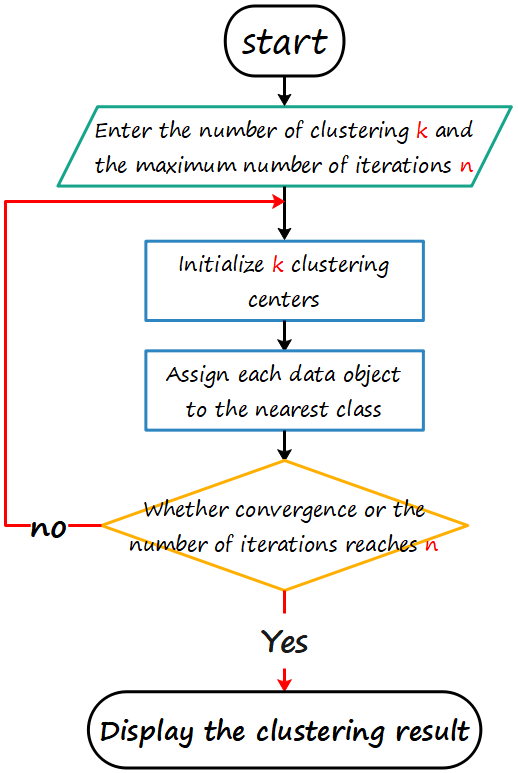
\includegraphics[width=.3\textwidth]{Q3_lct1.png}
	\caption{\small K-means flow chart}
\end{figure}

According to the number of player attempts as the clustering basis, the bungalow distance error and the degree of distortion between the particle of each cluster and the sample points within the cluster are called. Therefore, for a cluster, the lower the degree of distortion, the closer the members in the cluster, the higher the degree of distortion, the looser the structure in the cluster, and the degree of distortion will decrease with the increase of the category. However, for data with a certain degree of differentiation, the degree of distortion will be greatly improved when it reaches a certain near point, and then slowly decreases. This critical point can be considered as a point with better clustering performance.

\begin{figure}[htbp]
	\centering
	\begin{minipage}{0.45\linewidth}
		\centering
		\vspace{-0.6cm}
		\setlength{\abovecaptionskip}{0.28cm}
		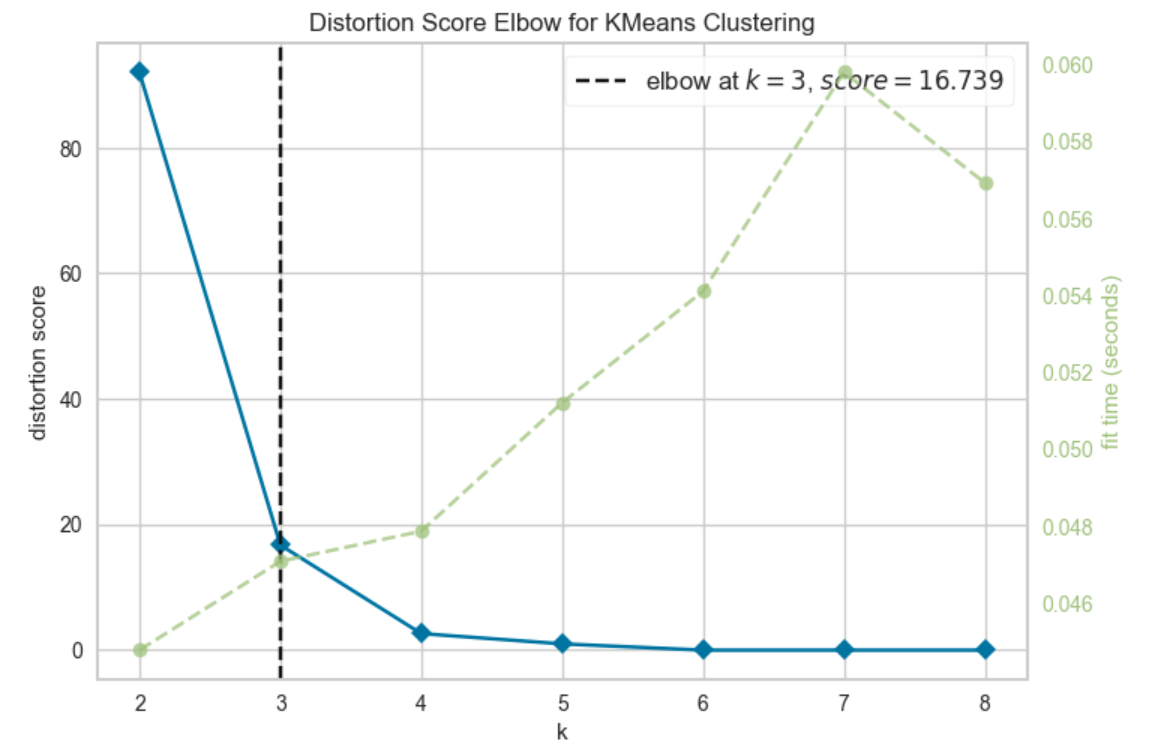
\includegraphics[width=\linewidth]{Q3_jlzx.png}
		\caption{\small K-means elbow chart}
		\label{fig:1}
	\end{minipage}
	%\qquad
	\hfill
	\begin{minipage}{0.45\linewidth}
		\centering
		\arrayrulecolor{light}
		\begin{tabular}{>{\columncolor{light}}lccc|}
			\hline
			 \rowcolor[gray]{0.85} & Easy & Middle & Diffcult \\ \hline
			1 try   & 1    & 0      & 0        \\ \hline 
			2 tries & 10   & 2      & 0        \\ \hline
			3 tries & 47   & 10     & 4        \\ \hline
			4 tries & 32   & 25     & 11       \\ \hline
			5 tries & 9    & 36     & 15       \\ \hline
			6 tries & 2    & 23     & 22       \\ \hline
			7 tries & 0    & 4      & 48      \\ \hline
		\end{tabular}
			\captionof{table}{\small Initial cluster center}%这里必须写table,不然标题就自动设置成figure
		\label{fig:NormalSafe}
	\end{minipage}
\end{figure}

From the figure above, it can be seen from the elbow rule that the clustering effect is optimal when there are three clustering centers. Therefore, we divide the words in the attachment into three categories: easy, medium and difficult. By K-means algorithm, we selected third, woken and parer as the initial clustering center of the three difficulties respectively. The number of attempts is shown as follows:

\subsection{Construction of difficulty evaluation model}
In order to provide a quantitative assessment standard for the difficulty of riddle words, we defined the word "difficulty" F as the measurement standard.
\begin{eqnarray}
	F  =  \frac{\sum_{x = 1}^{6} x \cdot N(x \text { tries })}{\sum_{x  =  1}^{6} N(x \text { tries })}
\end{eqnarray}

Where $x$ is the number of times it took the player to guess the answer to the riddle.

By quantifying the difficulty, we calculated the difficulty of all the words in the sample data. The difficulty level of the three clustering centers selected during classification is used as the standard for quantitative evaluation of word difficulty classification. See appendix for the difficulty table:


The following figure is the kernel density estimation chart of the percentage of different attempts divided according to clustering. It can be intuitively seen that the data is obviously divided into three categories, indicating that the clustering summary model of K-means is excellent.
\begin{figure*}[htbp] %通栏
	\begin{minipage}[t]{0.33\linewidth} %调节两个子图左右间距
		\centering
		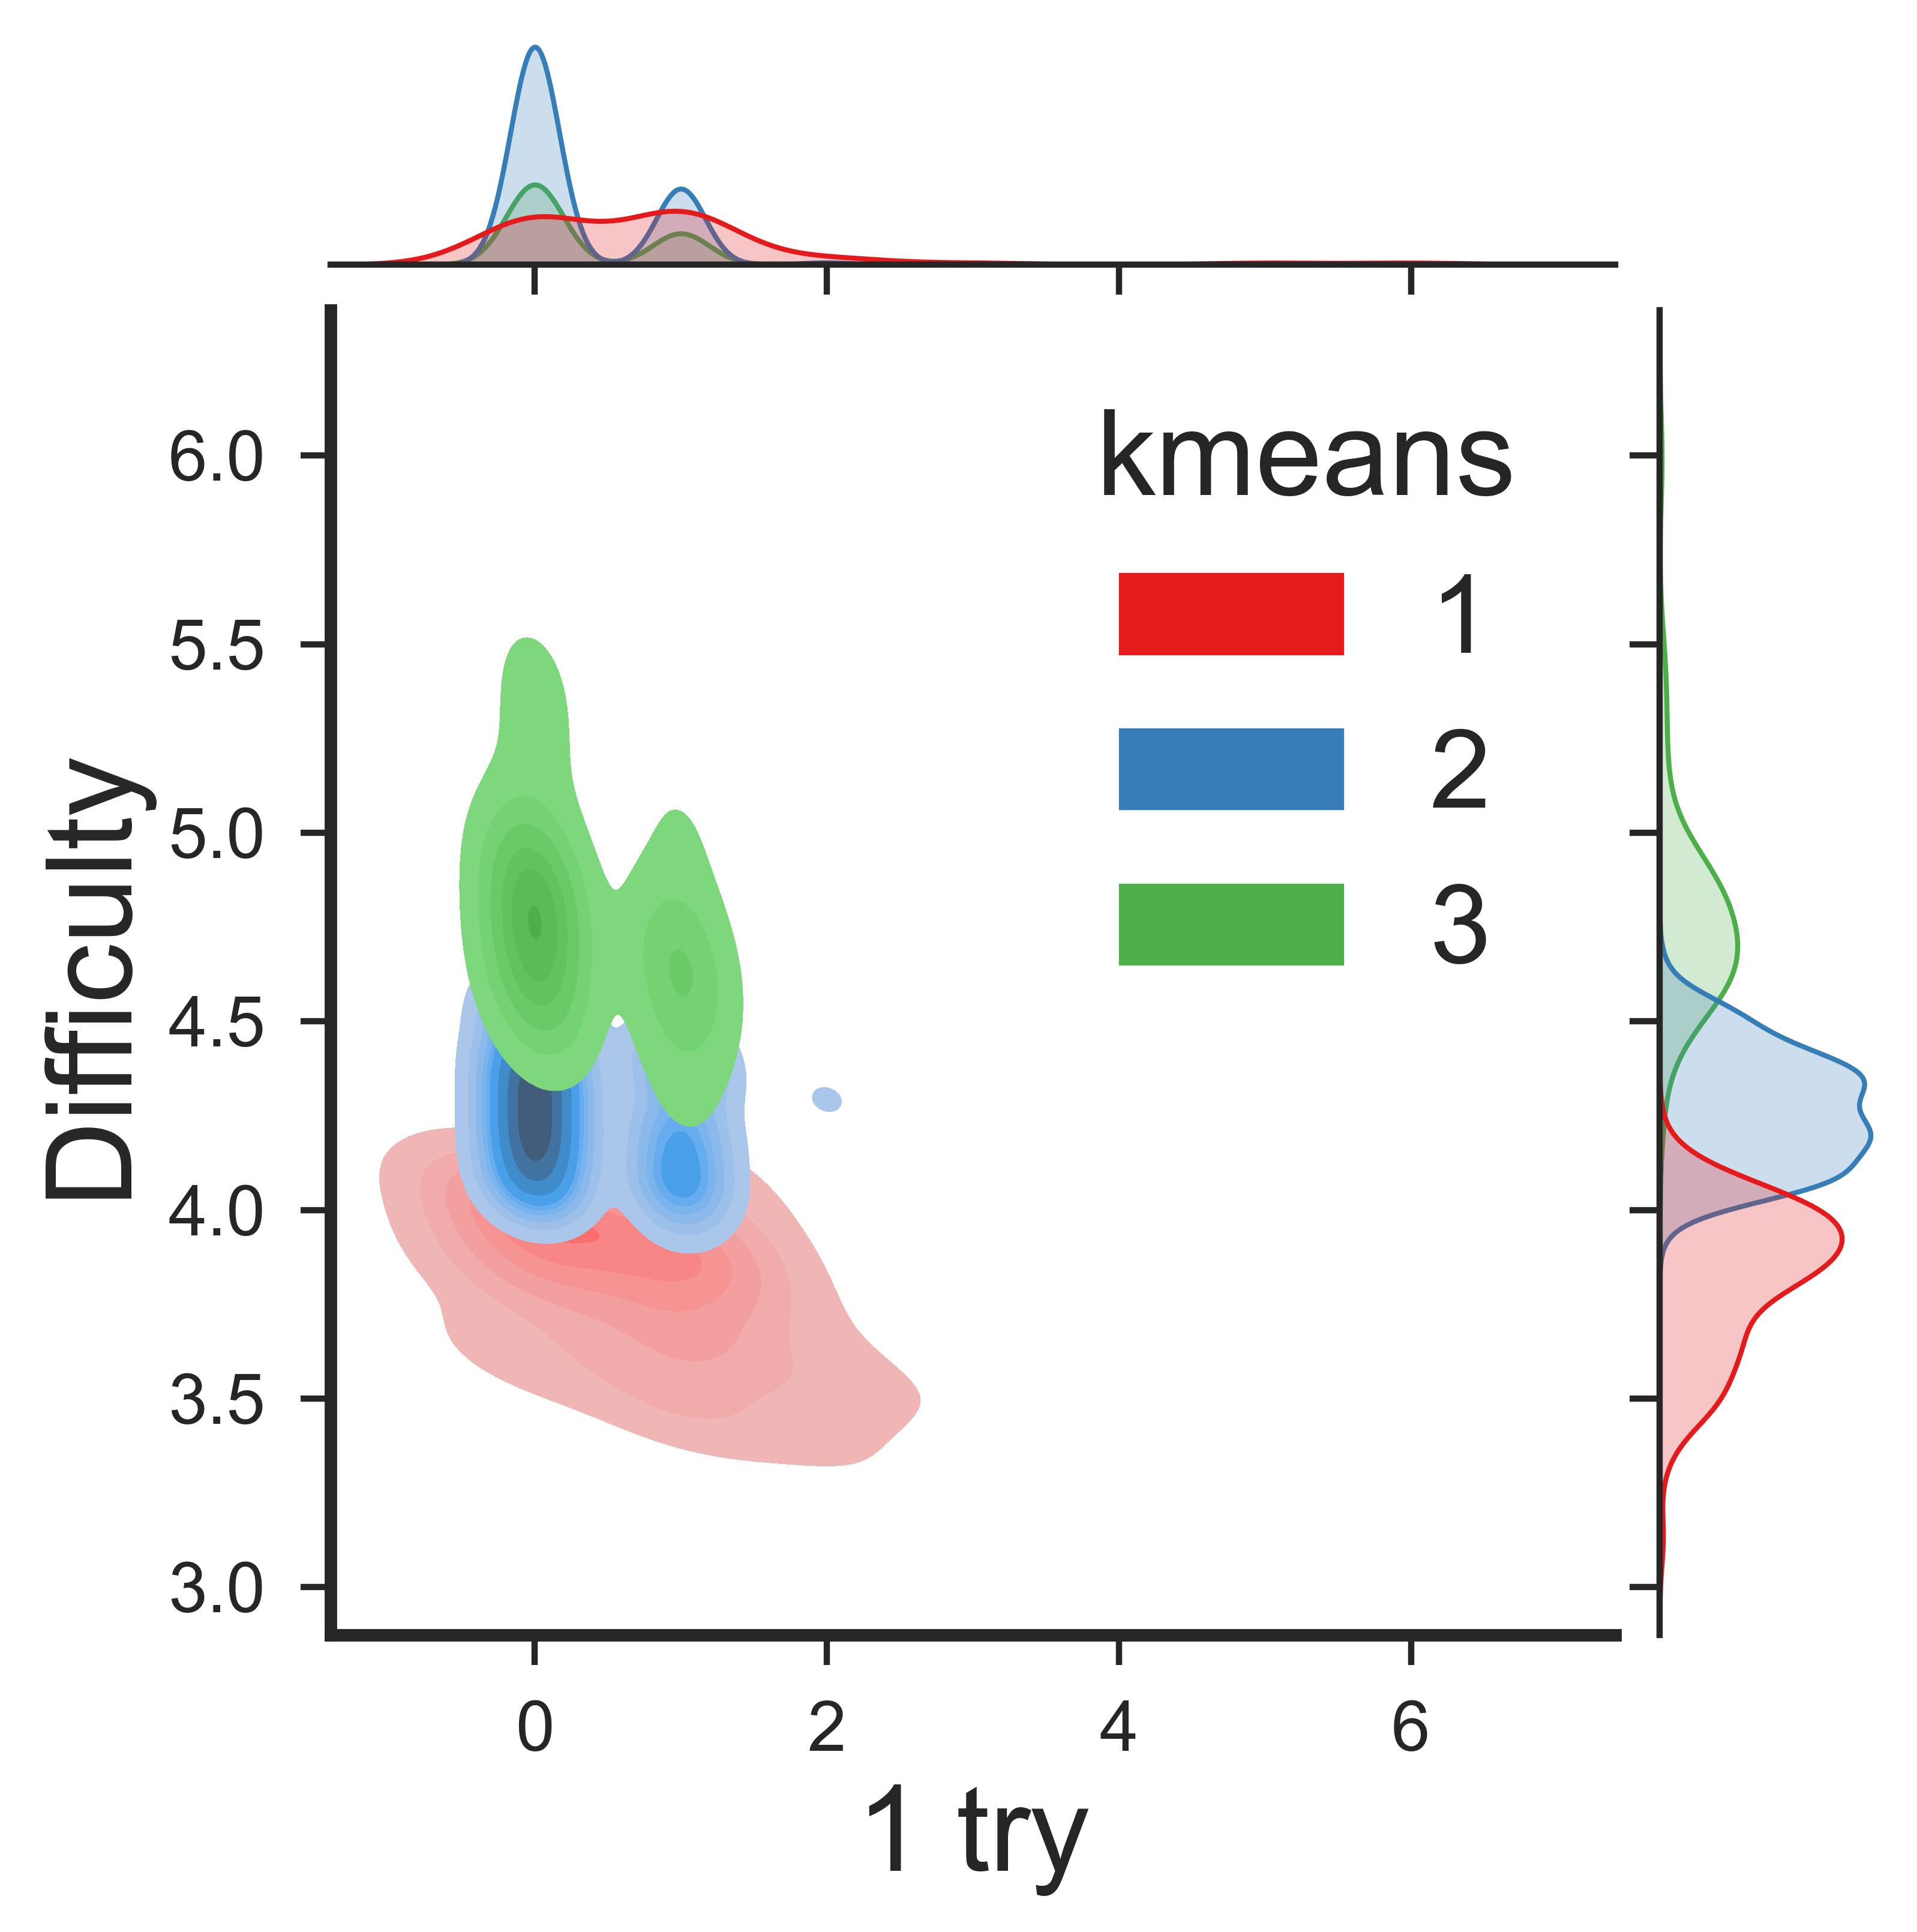
\includegraphics[width=1.9in, height=1.9in]{1_try_difficulty.jpg} %调节单个子图大小
	\end{minipage}%
	\begin{minipage}[t]{0.33\linewidth}
		\centering
		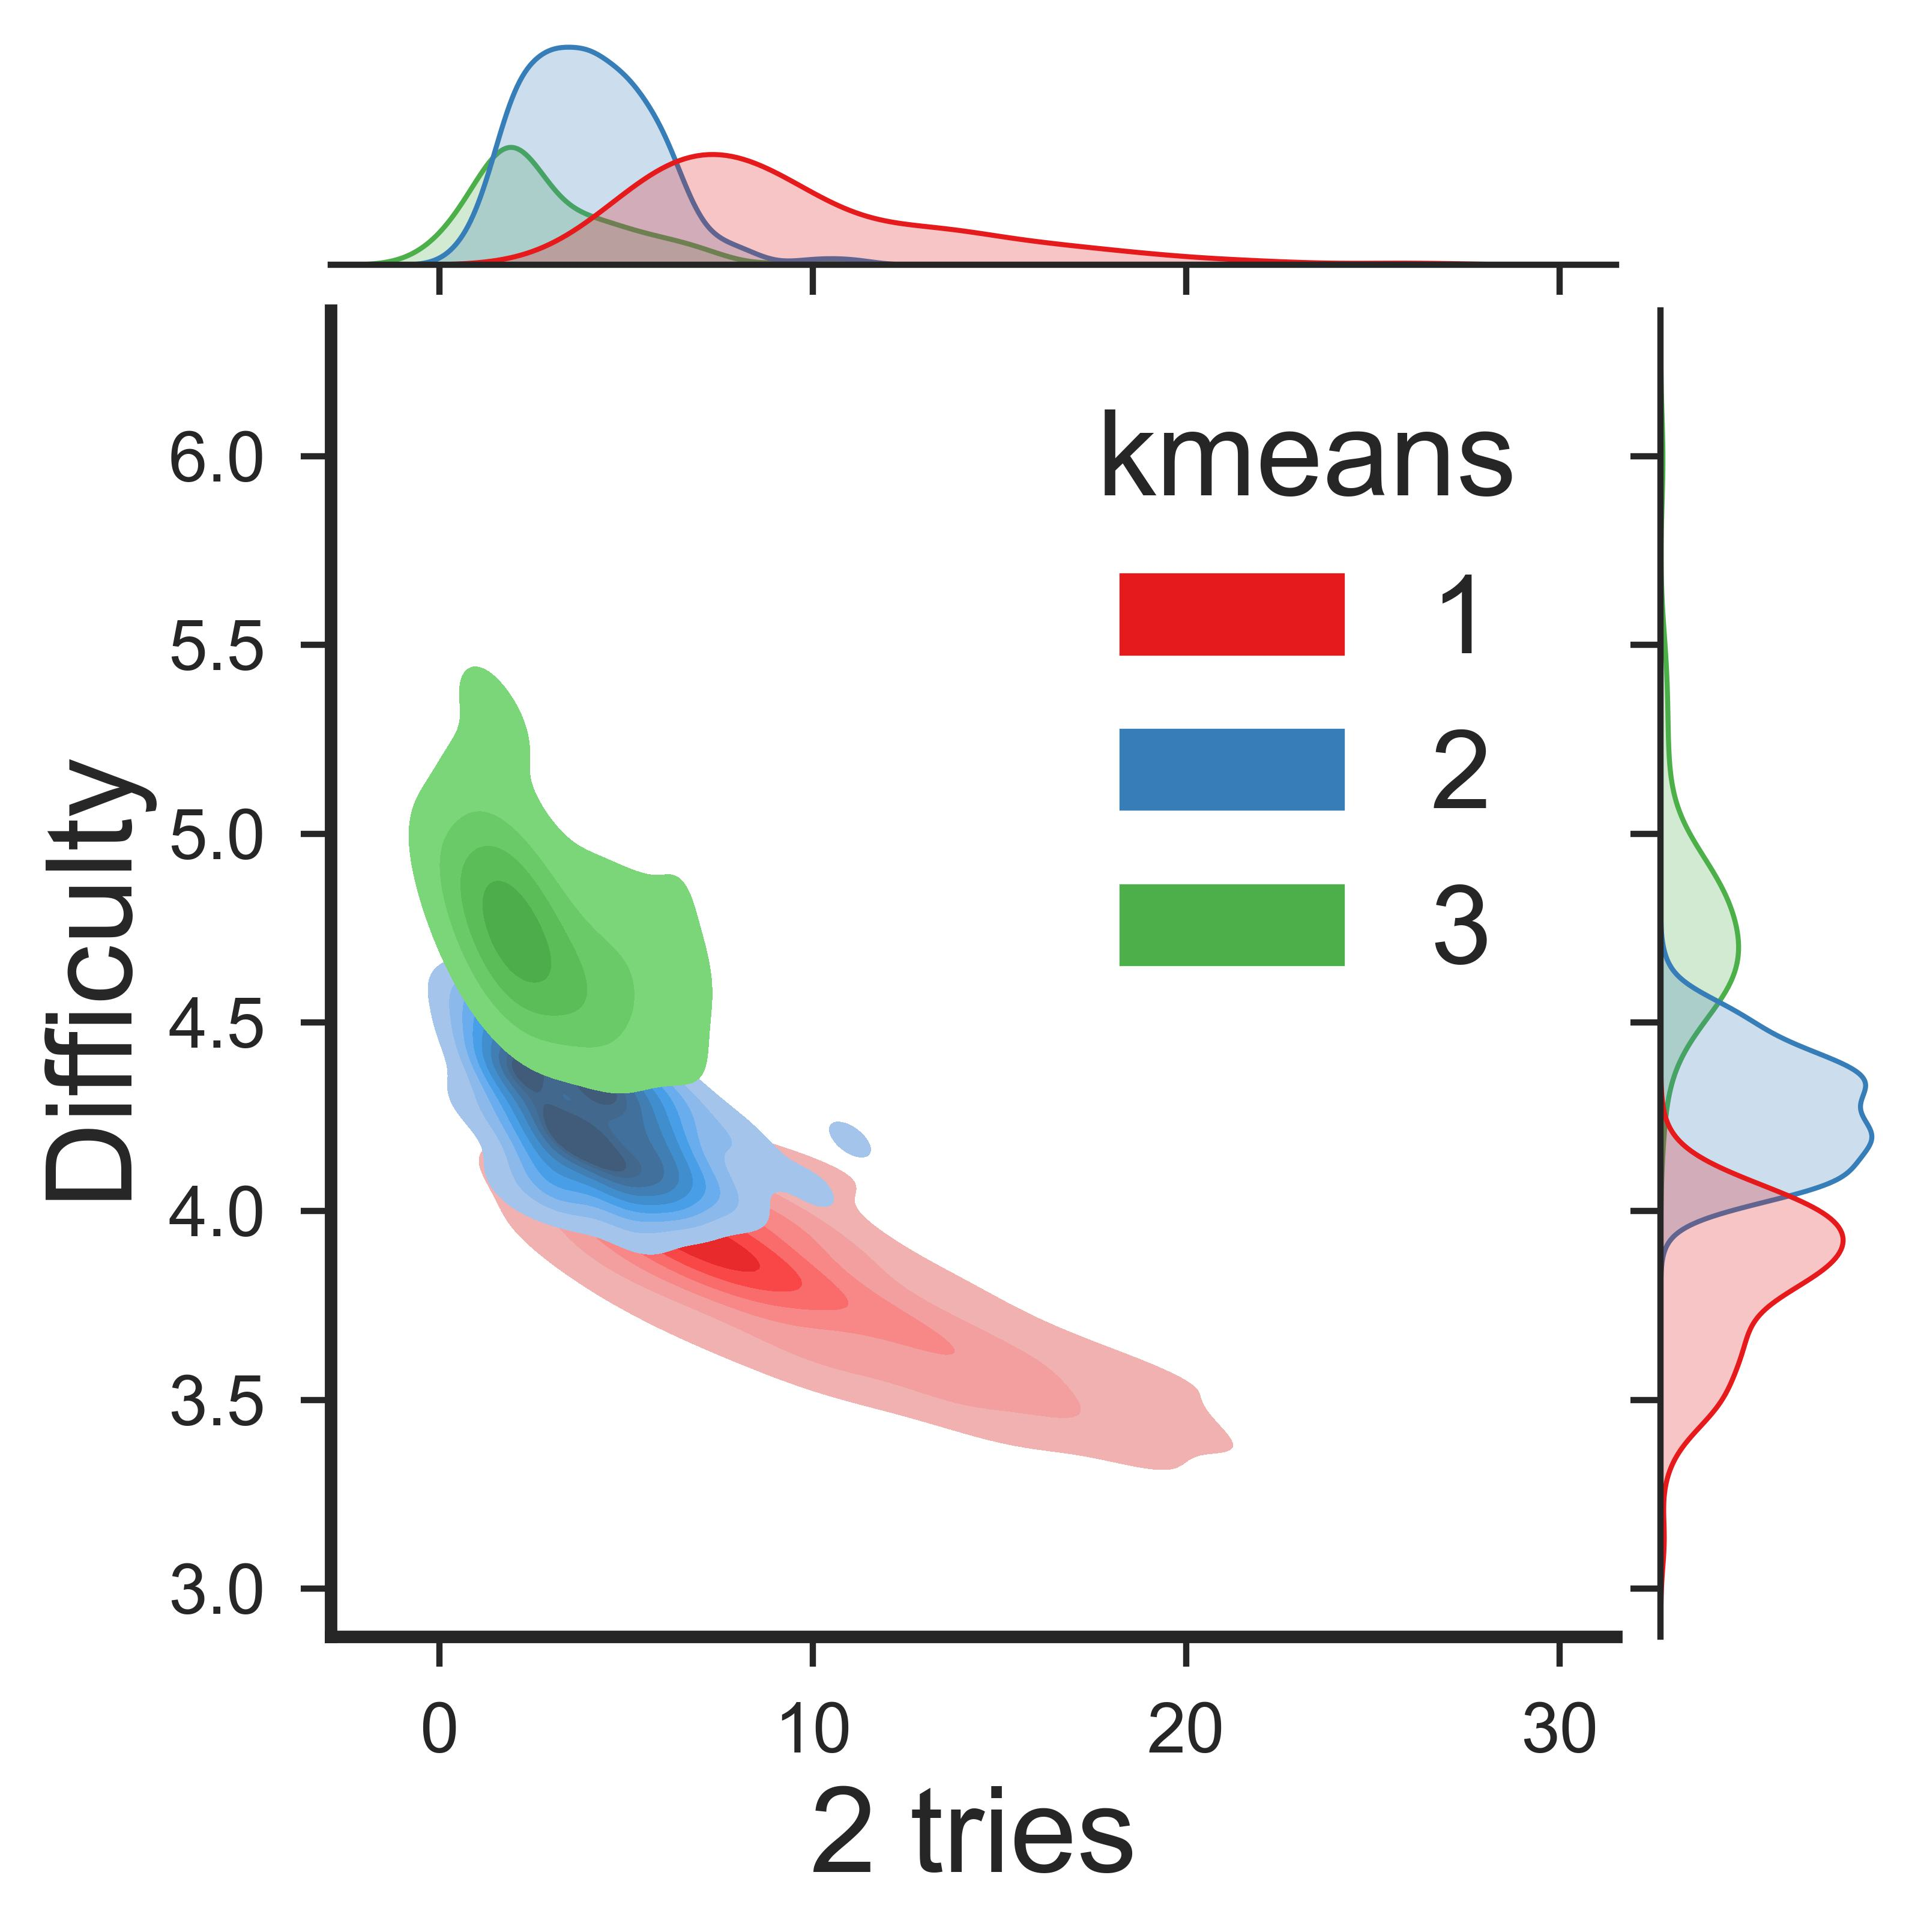
\includegraphics[width=1.9in, height=1.9in]{2_try-difficulty.jpg}
	\end{minipage}%
	\begin{minipage}[t]{0.33\linewidth}
		\centering
		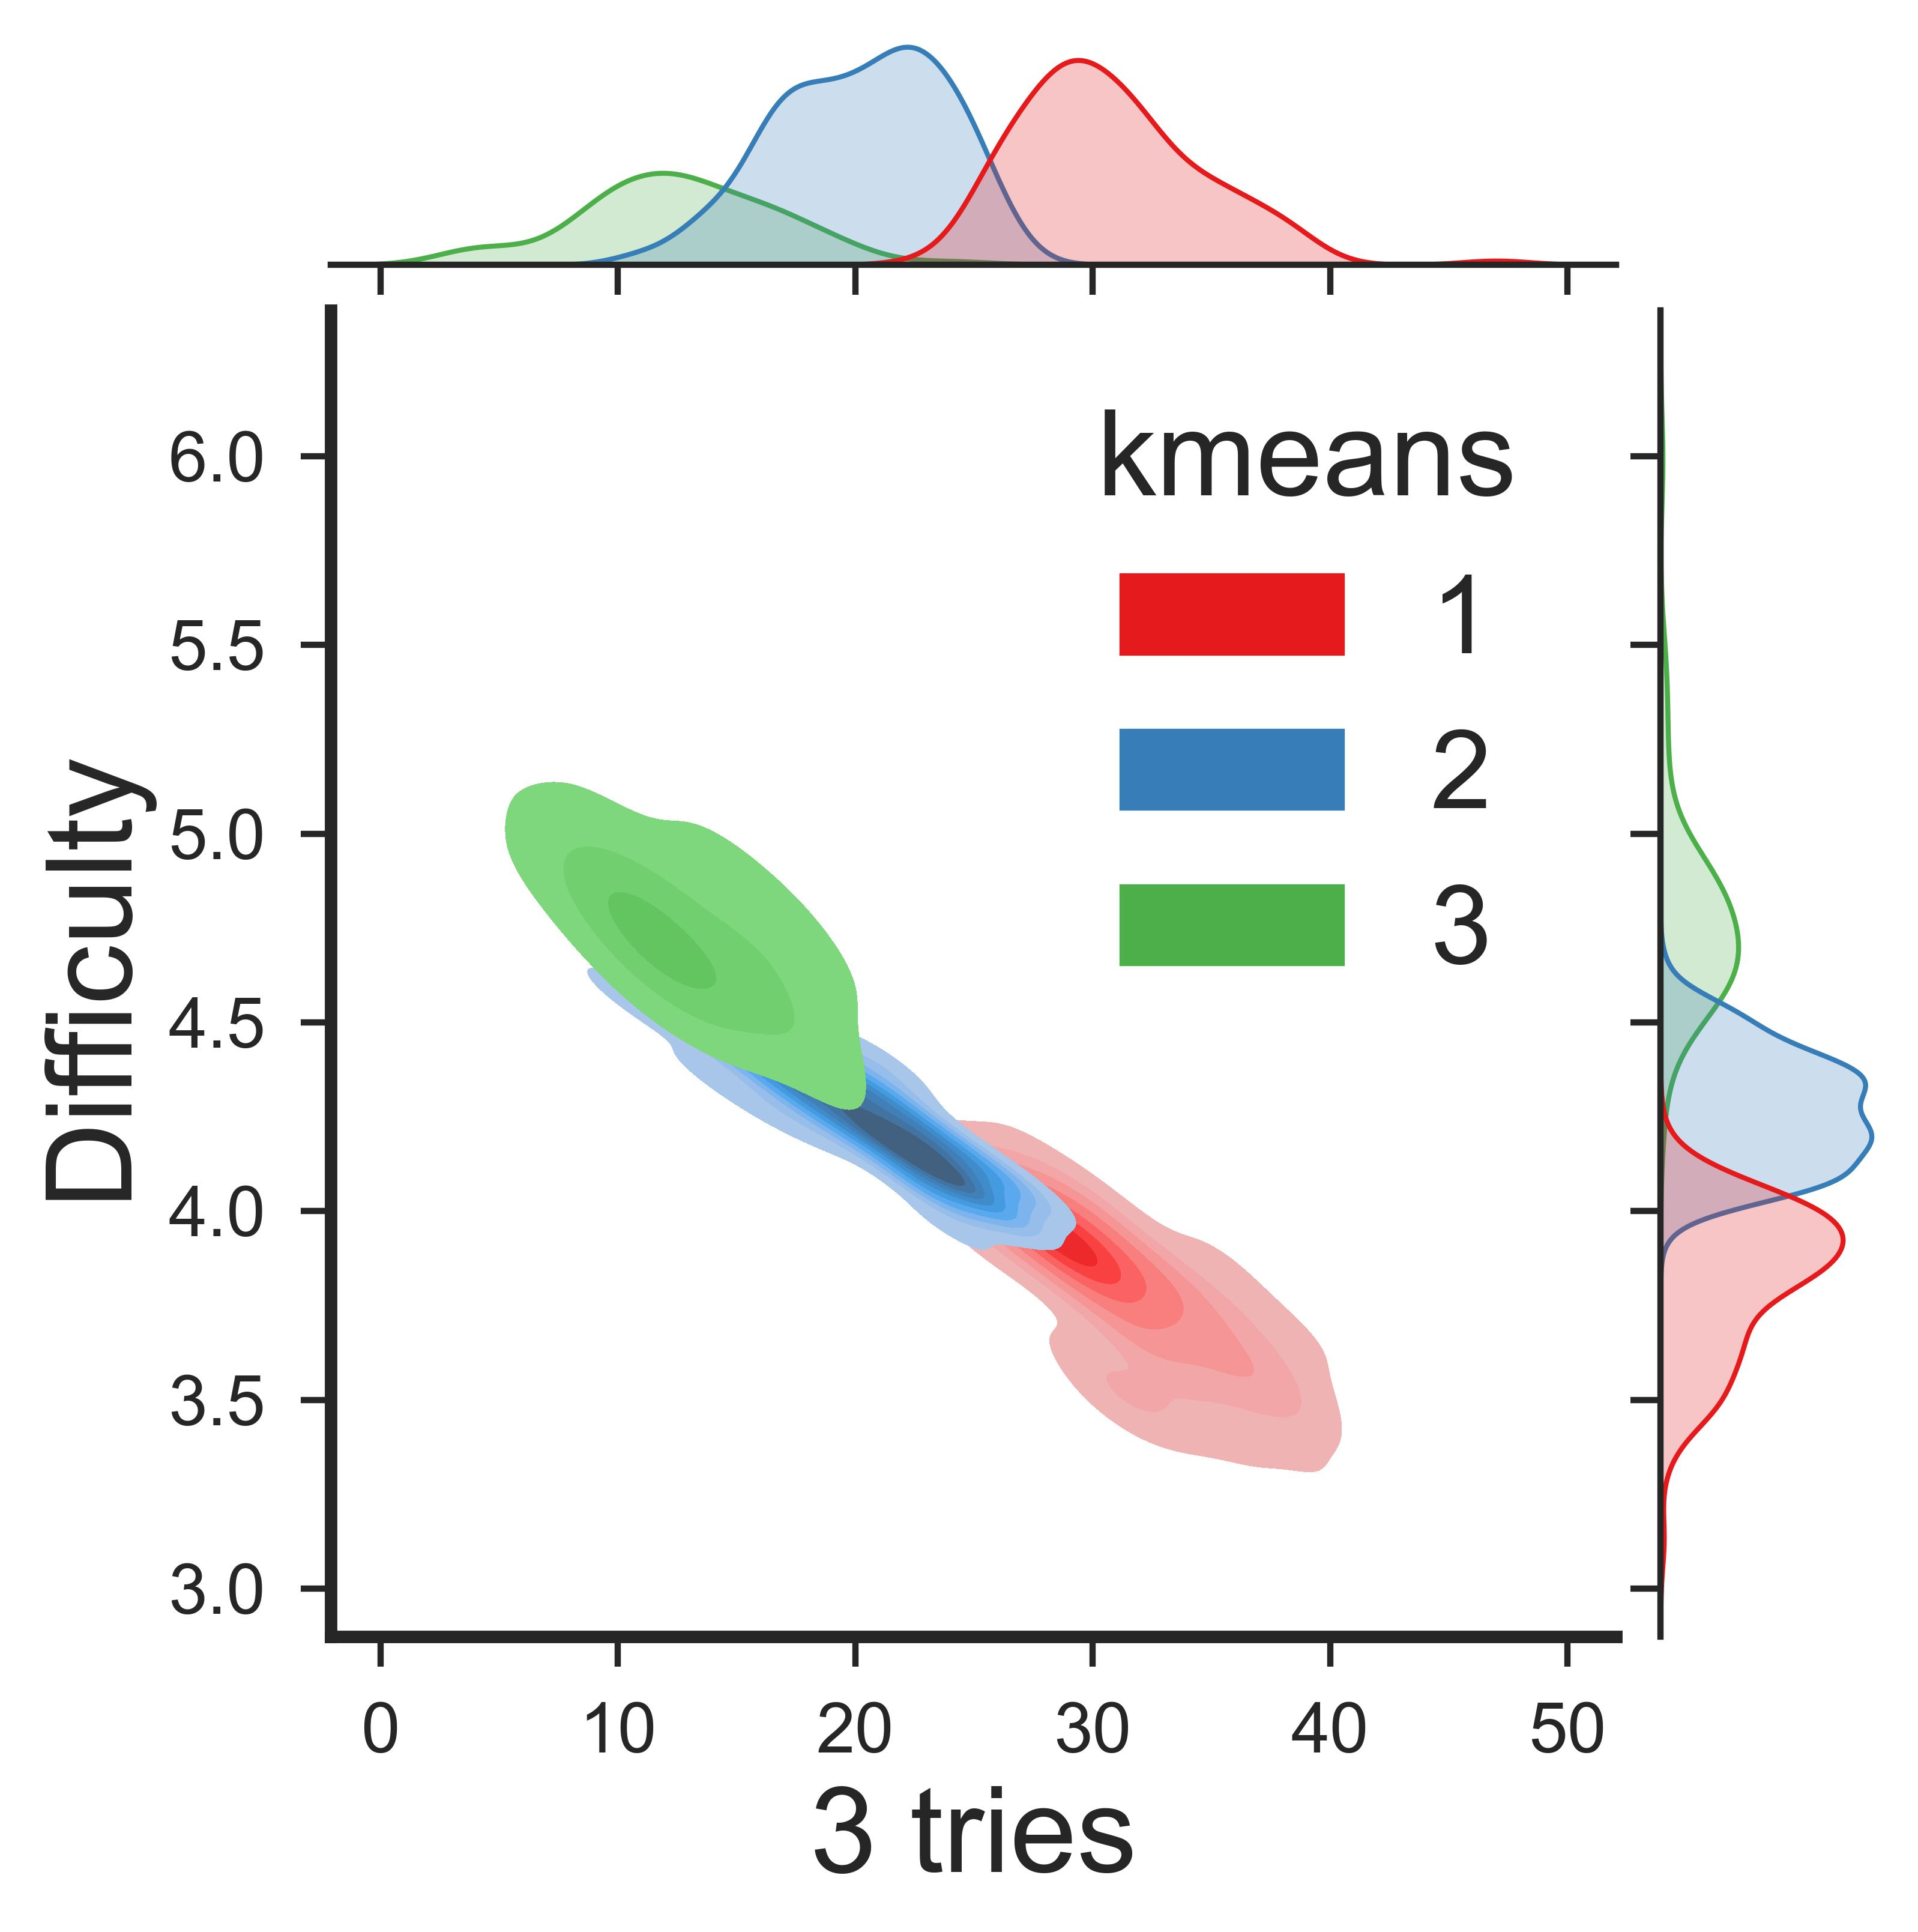
\includegraphics[width=1.9in, height=1.9in]{3_try-difficulty.jpg}
	\end{minipage}
\end{figure*}
\begin{figure*}[htbp] %通栏
	\begin{minipage}[t]{0.33\linewidth} %调节两个子图左右间距
		\centering
		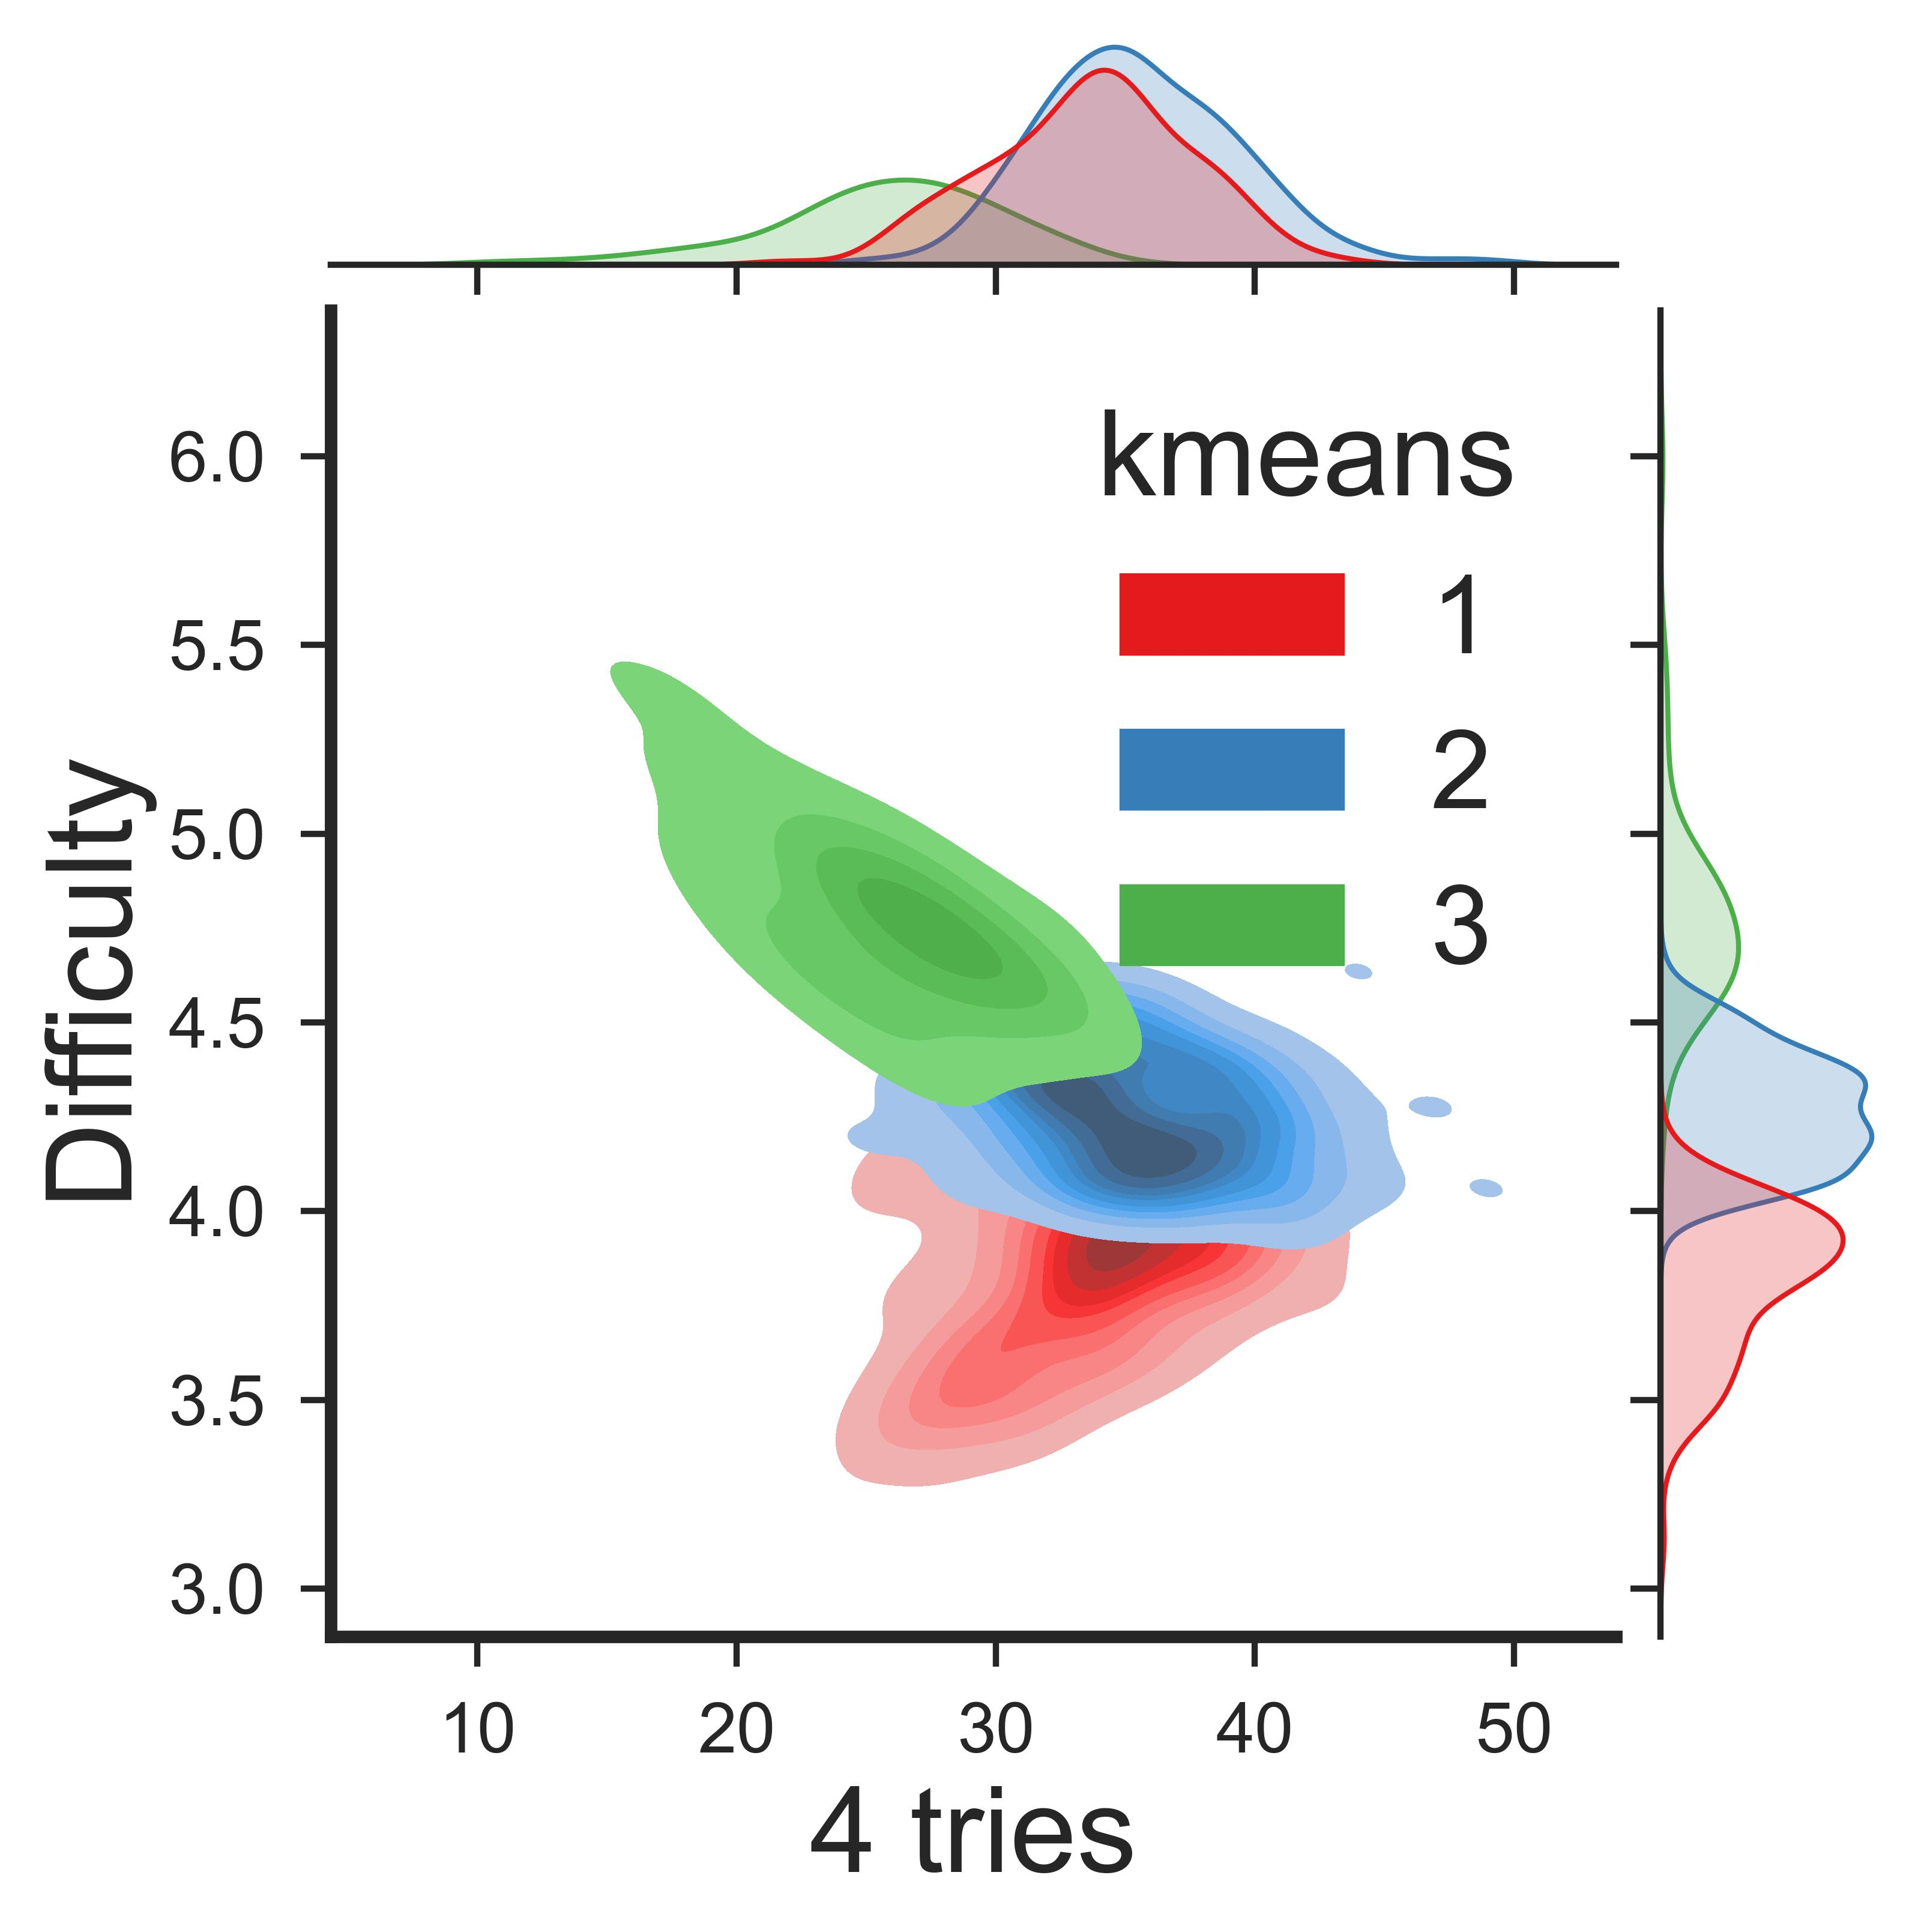
\includegraphics[width=1.9in, height=1.9in]{4_try-difficulty.jpg} %调节单个子图大小
	\end{minipage}%
	\begin{minipage}[t]{0.33\linewidth}
		\centering
		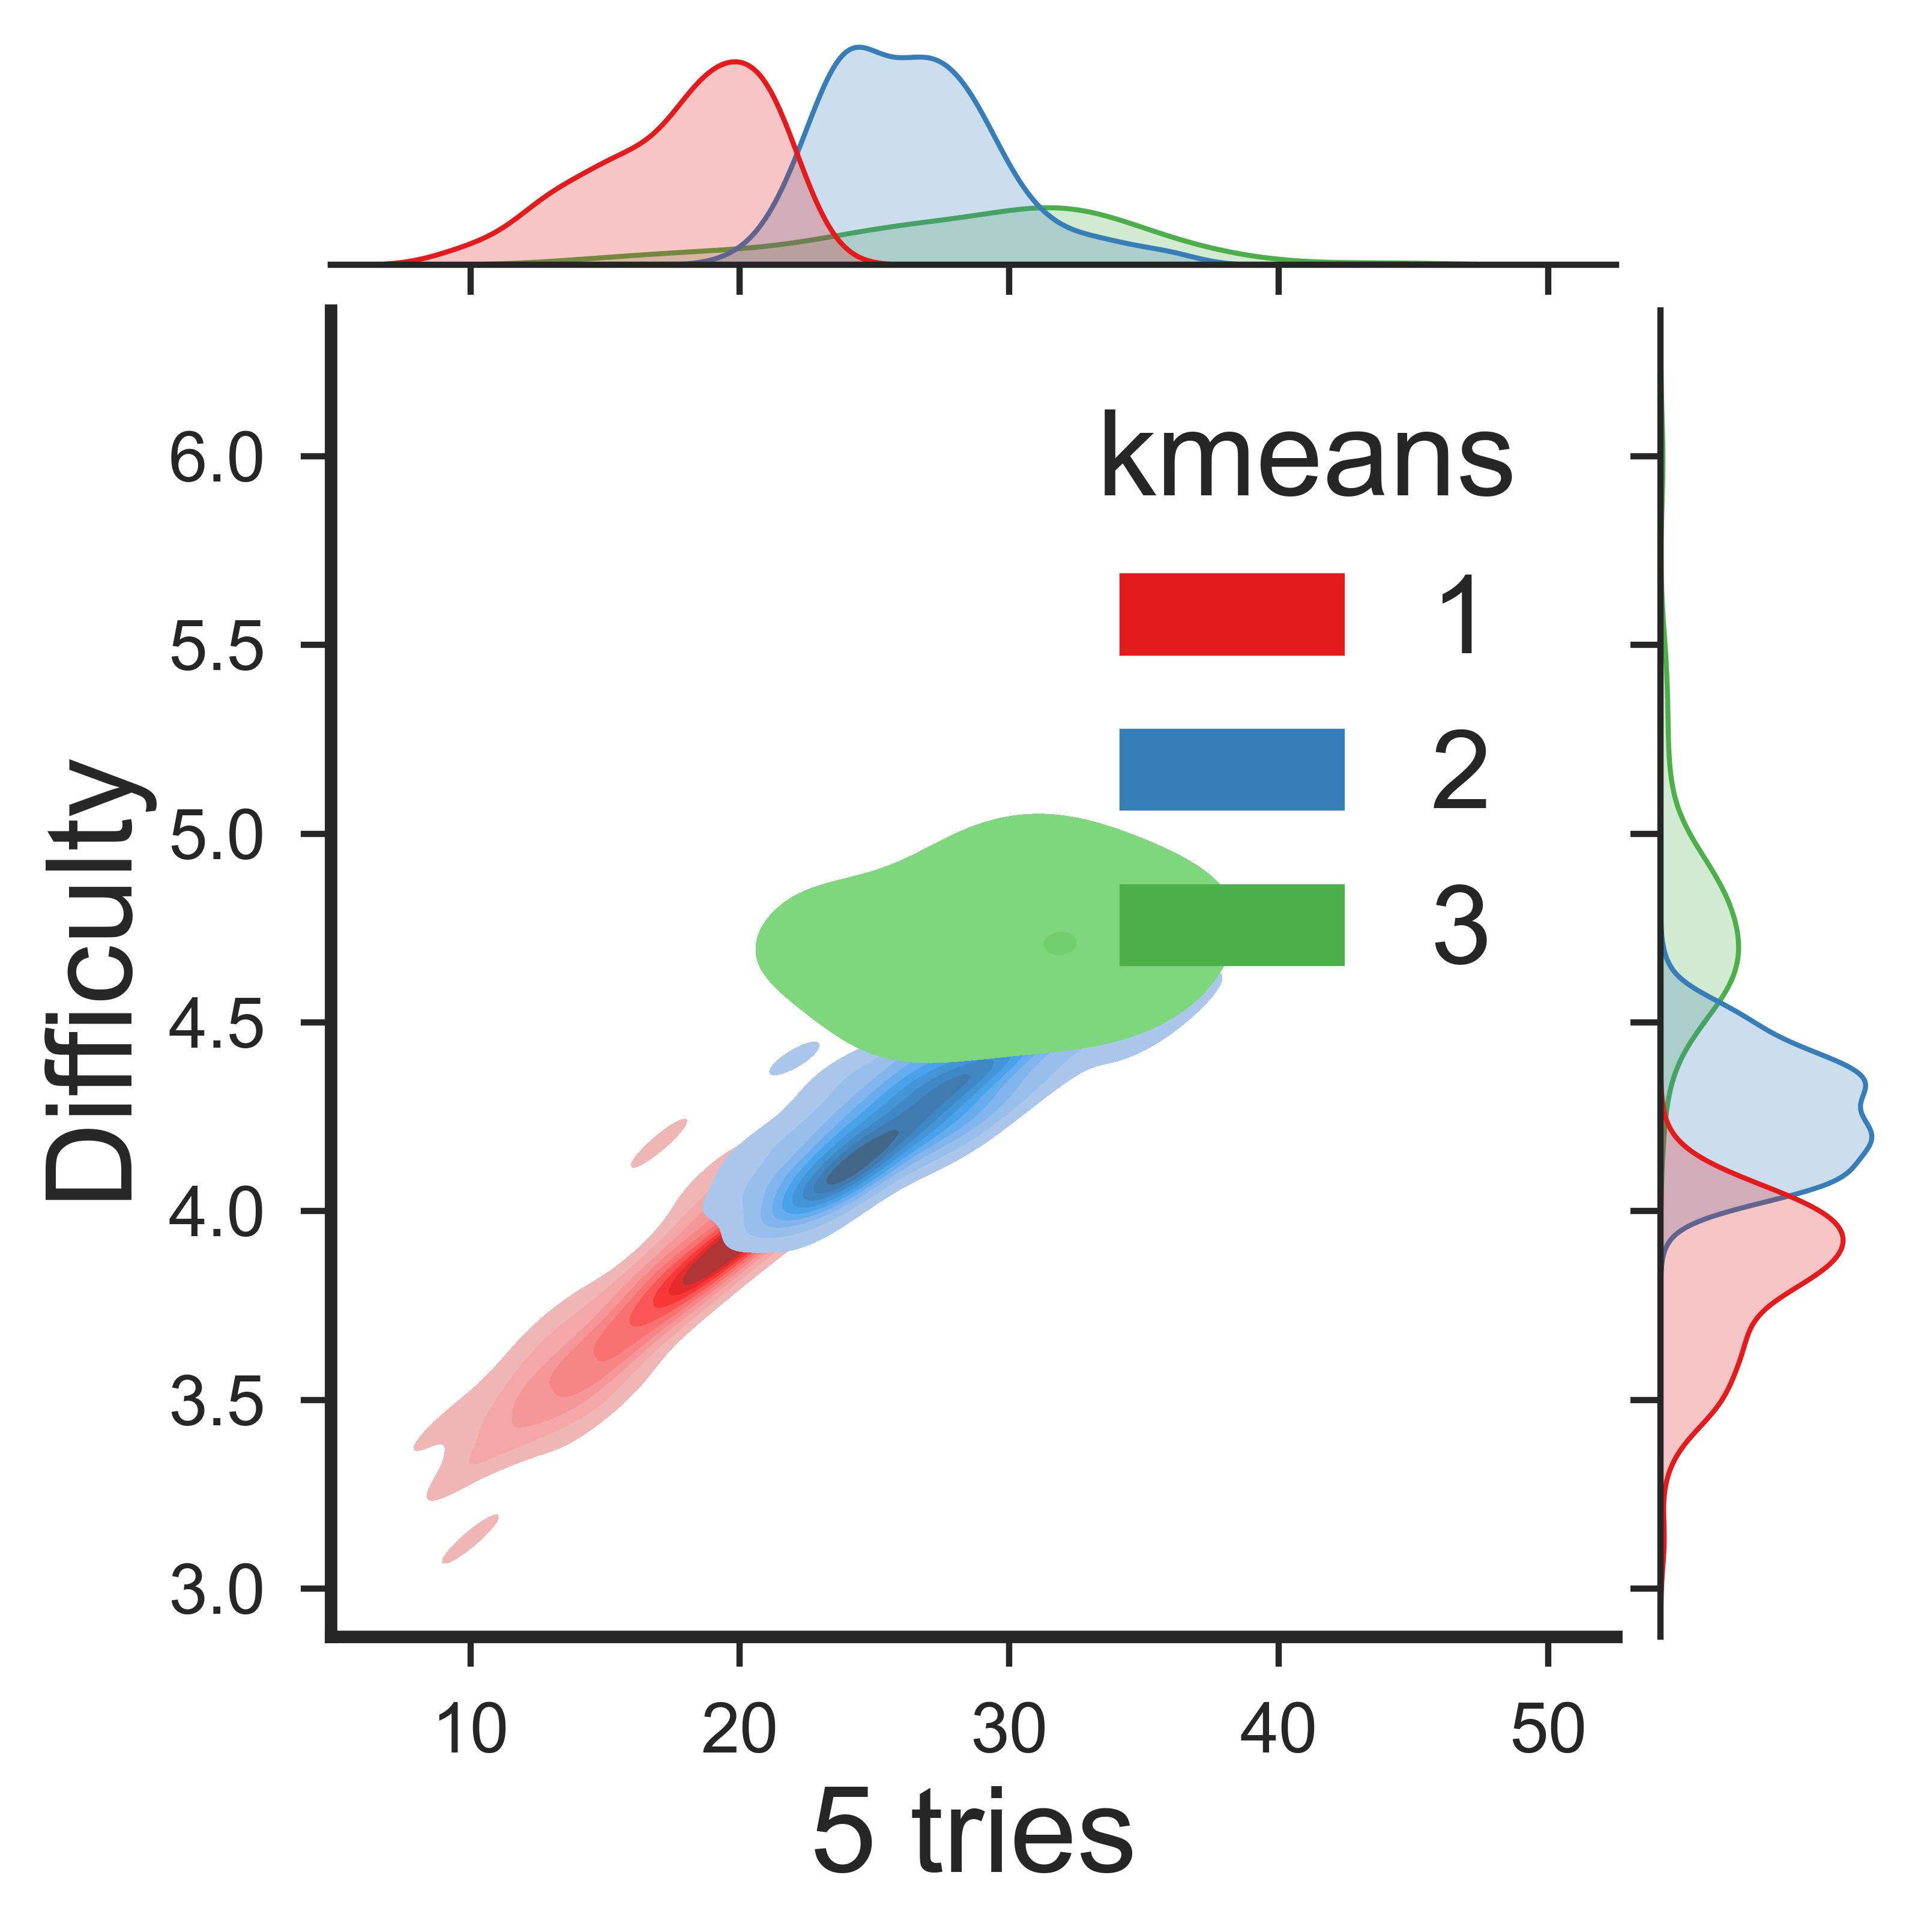
\includegraphics[width=1.9in, height=1.9in]{5_try-difficulty.jpg}
	\end{minipage}%
	\begin{minipage}[t]{0.33\linewidth}
		\centering
		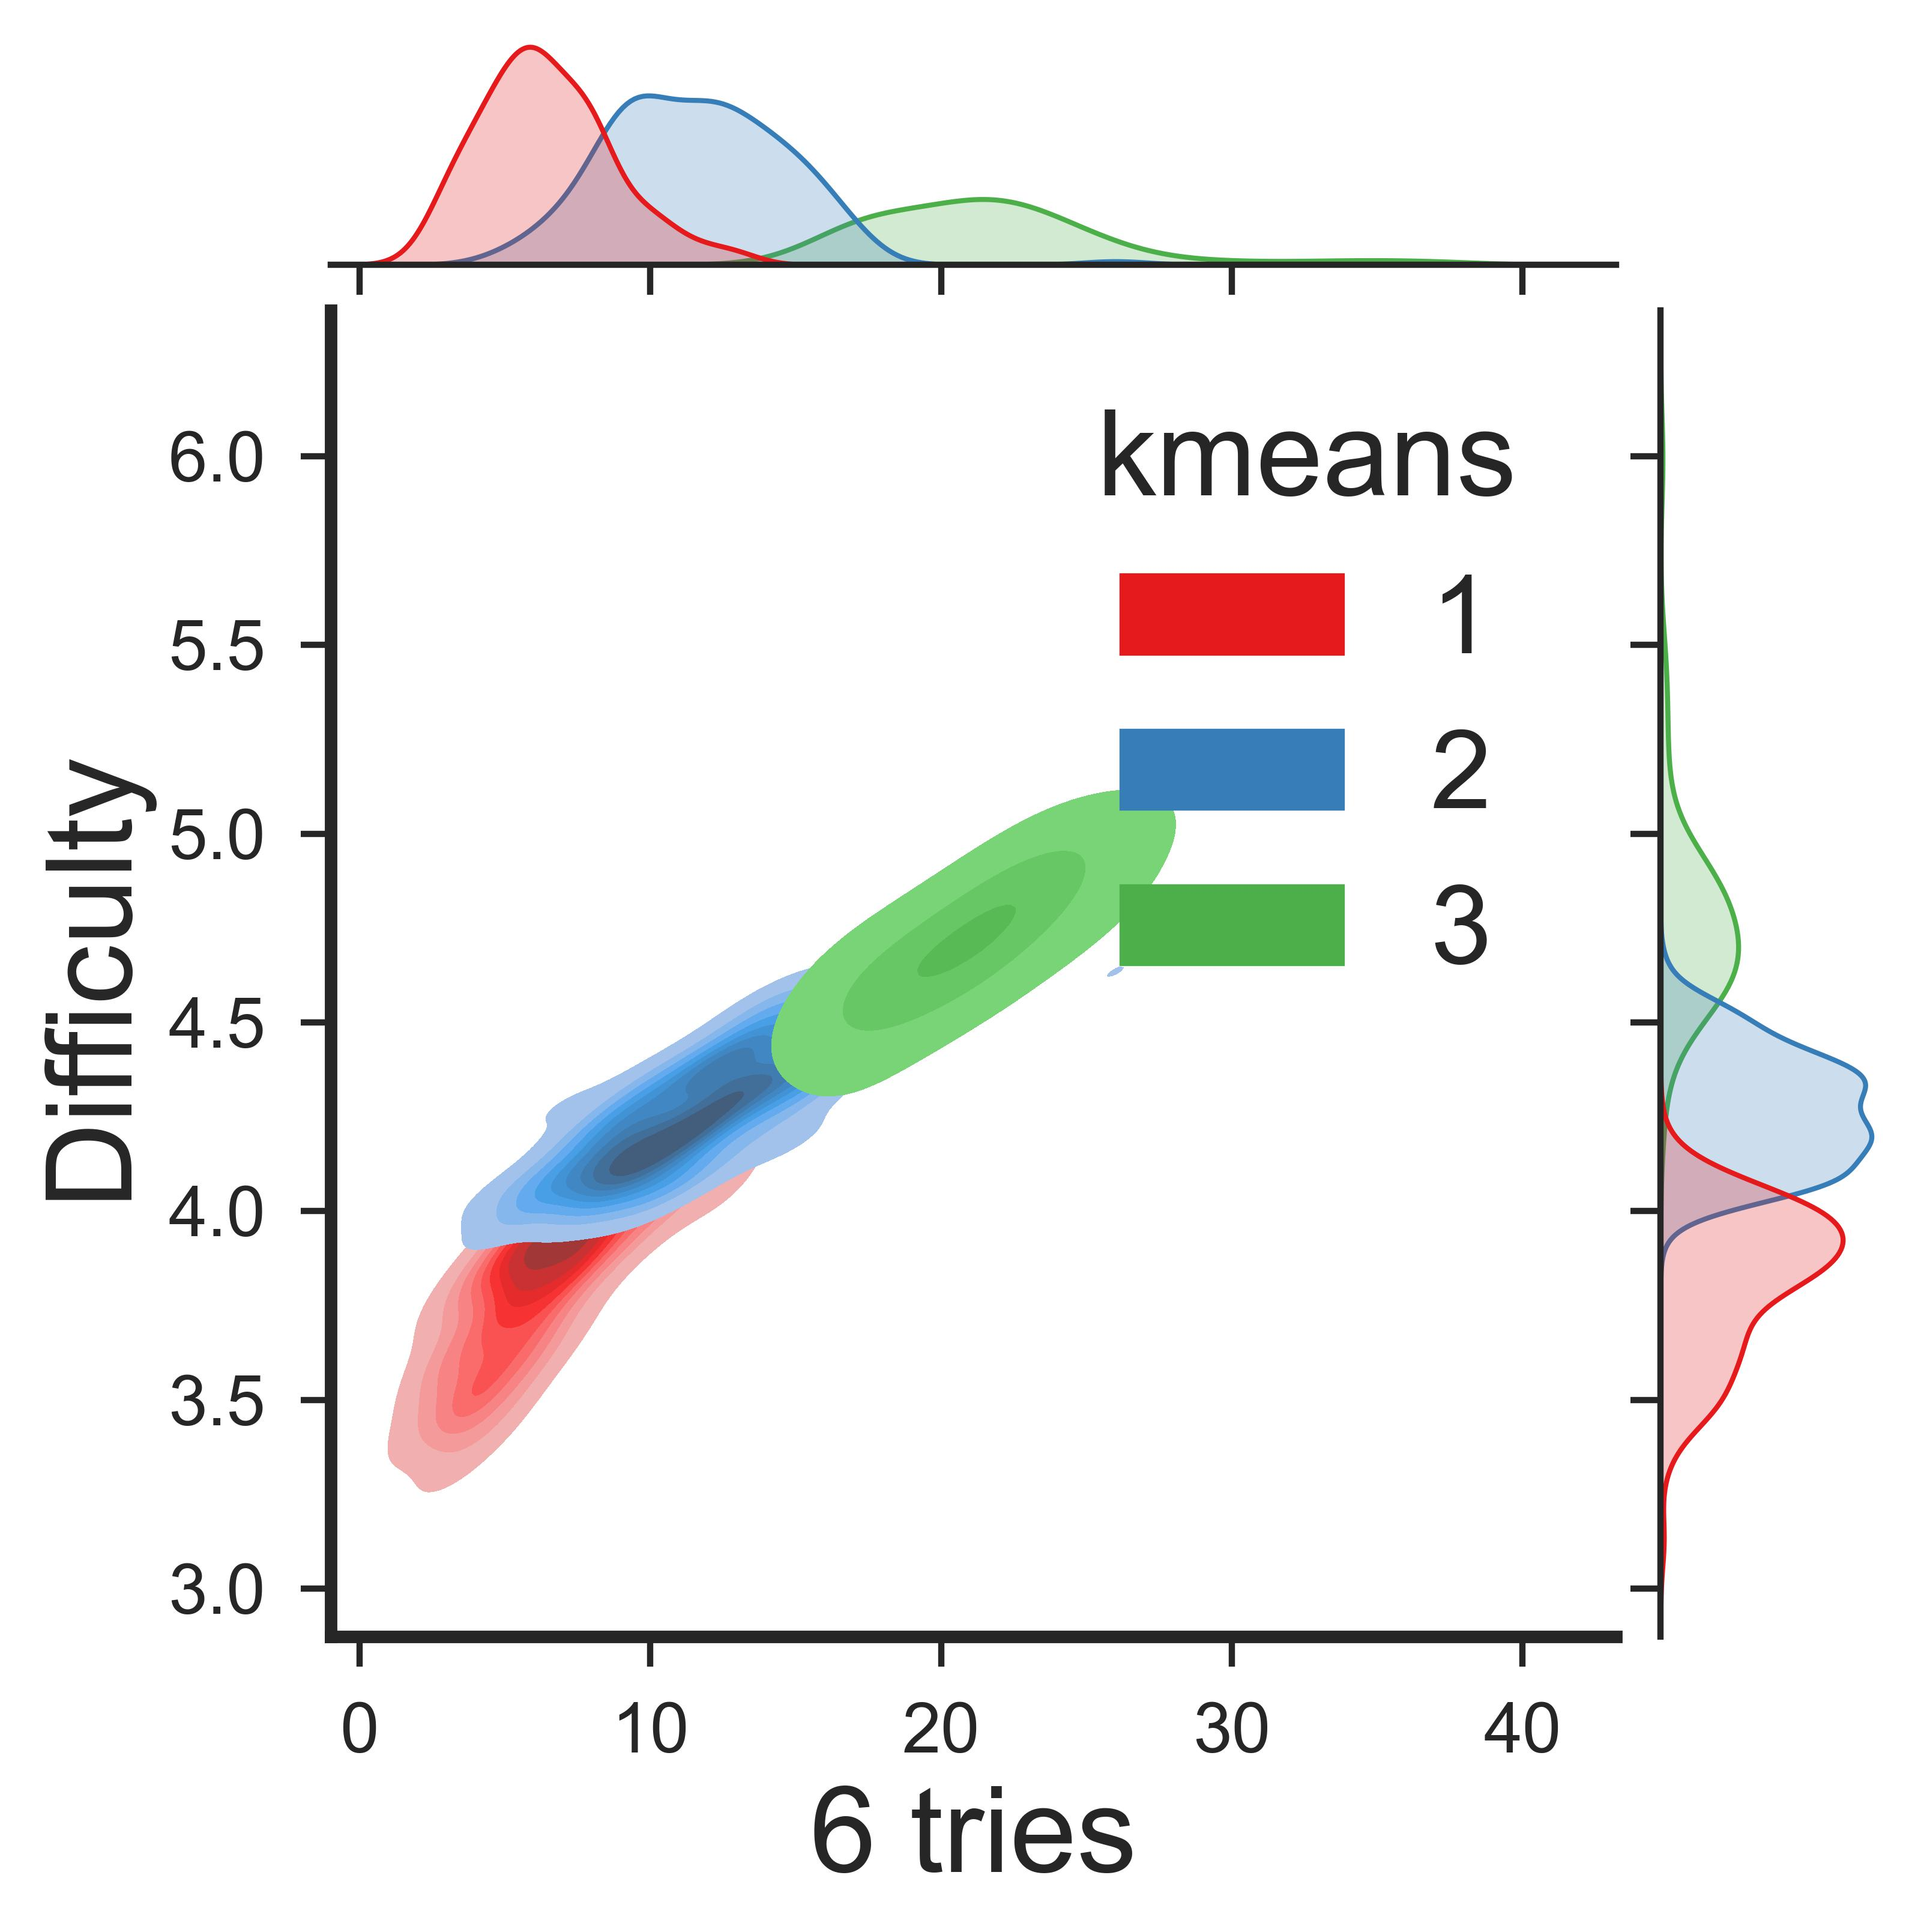
\includegraphics[width=1.9in, height=1.9in]{6_try-difficulty.jpg}
	\end{minipage}
\end{figure*}

Then we took the percentage of each attempt as the independent variable and the clustering result as the dependent variable. The first 90\% of the sample data in the attachment is taken as the training set, and the last 10\% is taken as the test set. BP neural network classification is carried out on the data.

\subsection{Verification of classification evaluation model}
In order to verify the accuracy of classification results, we cross-validate the classification results of bp neural network. When the accuracy rate is 99\%, the recall rate is also 99\%, indicating that the model is very excellent. Even in the case of incomplete sample size, it still has a high classification effect, and we believe that the difficulty evaluation classification model built by us has a good effect. The specific results are as follows:
\begin{table}[H]
	\centering
	\arrayrulecolor{black}
	\renewcommand\arraystretch{1.1}
	\caption{\small BP model evaluation}
	\begin{tabular}{cccc}
		\toprule[1.5pt]
		\makebox[0.2\textwidth][c]{BP} & \makebox[0.2\textwidth][c]{Accuracy rate} & \makebox[0.2\textwidth][c]{Recall rate}
		& \makebox[0.2\textwidth][c]{F1} \\
		\midrule[1.5pt]
		Training set & 1             & 1           & 1     \\
Test set     & 0.992         & 0.989       & 0.991 \\
		\bottomrule[1.5pt]
	\end{tabular}
\end{table}

\subsection{EERIE difficulty prediction}
Through the model of problem two, we have completed the guessing situation of the players in Wordle when the word EERIE is used as the answer to the riddle. According to the difficulty evaluation system we constructed, the difficulty level of this word is calculated as $F(EERIE)=5.03$, thus indicating that the difficulty level of this word is difficult.

\section{Some interesting discovery}
\noindent
\textbf{6.1 Percentage increase in hard mode}

Interestingly, although the Number of reported result decreased over time, the number of players participating in difficult mode increased steadily. The following is the trend plot and linear regression residual plot of the number of players participating in difficult mode, the percentage of total players and the Contest number:
\begin{figure}[H]
	\subfigure
	{
		\begin{minipage}[b]{.28\linewidth}
			\centering
			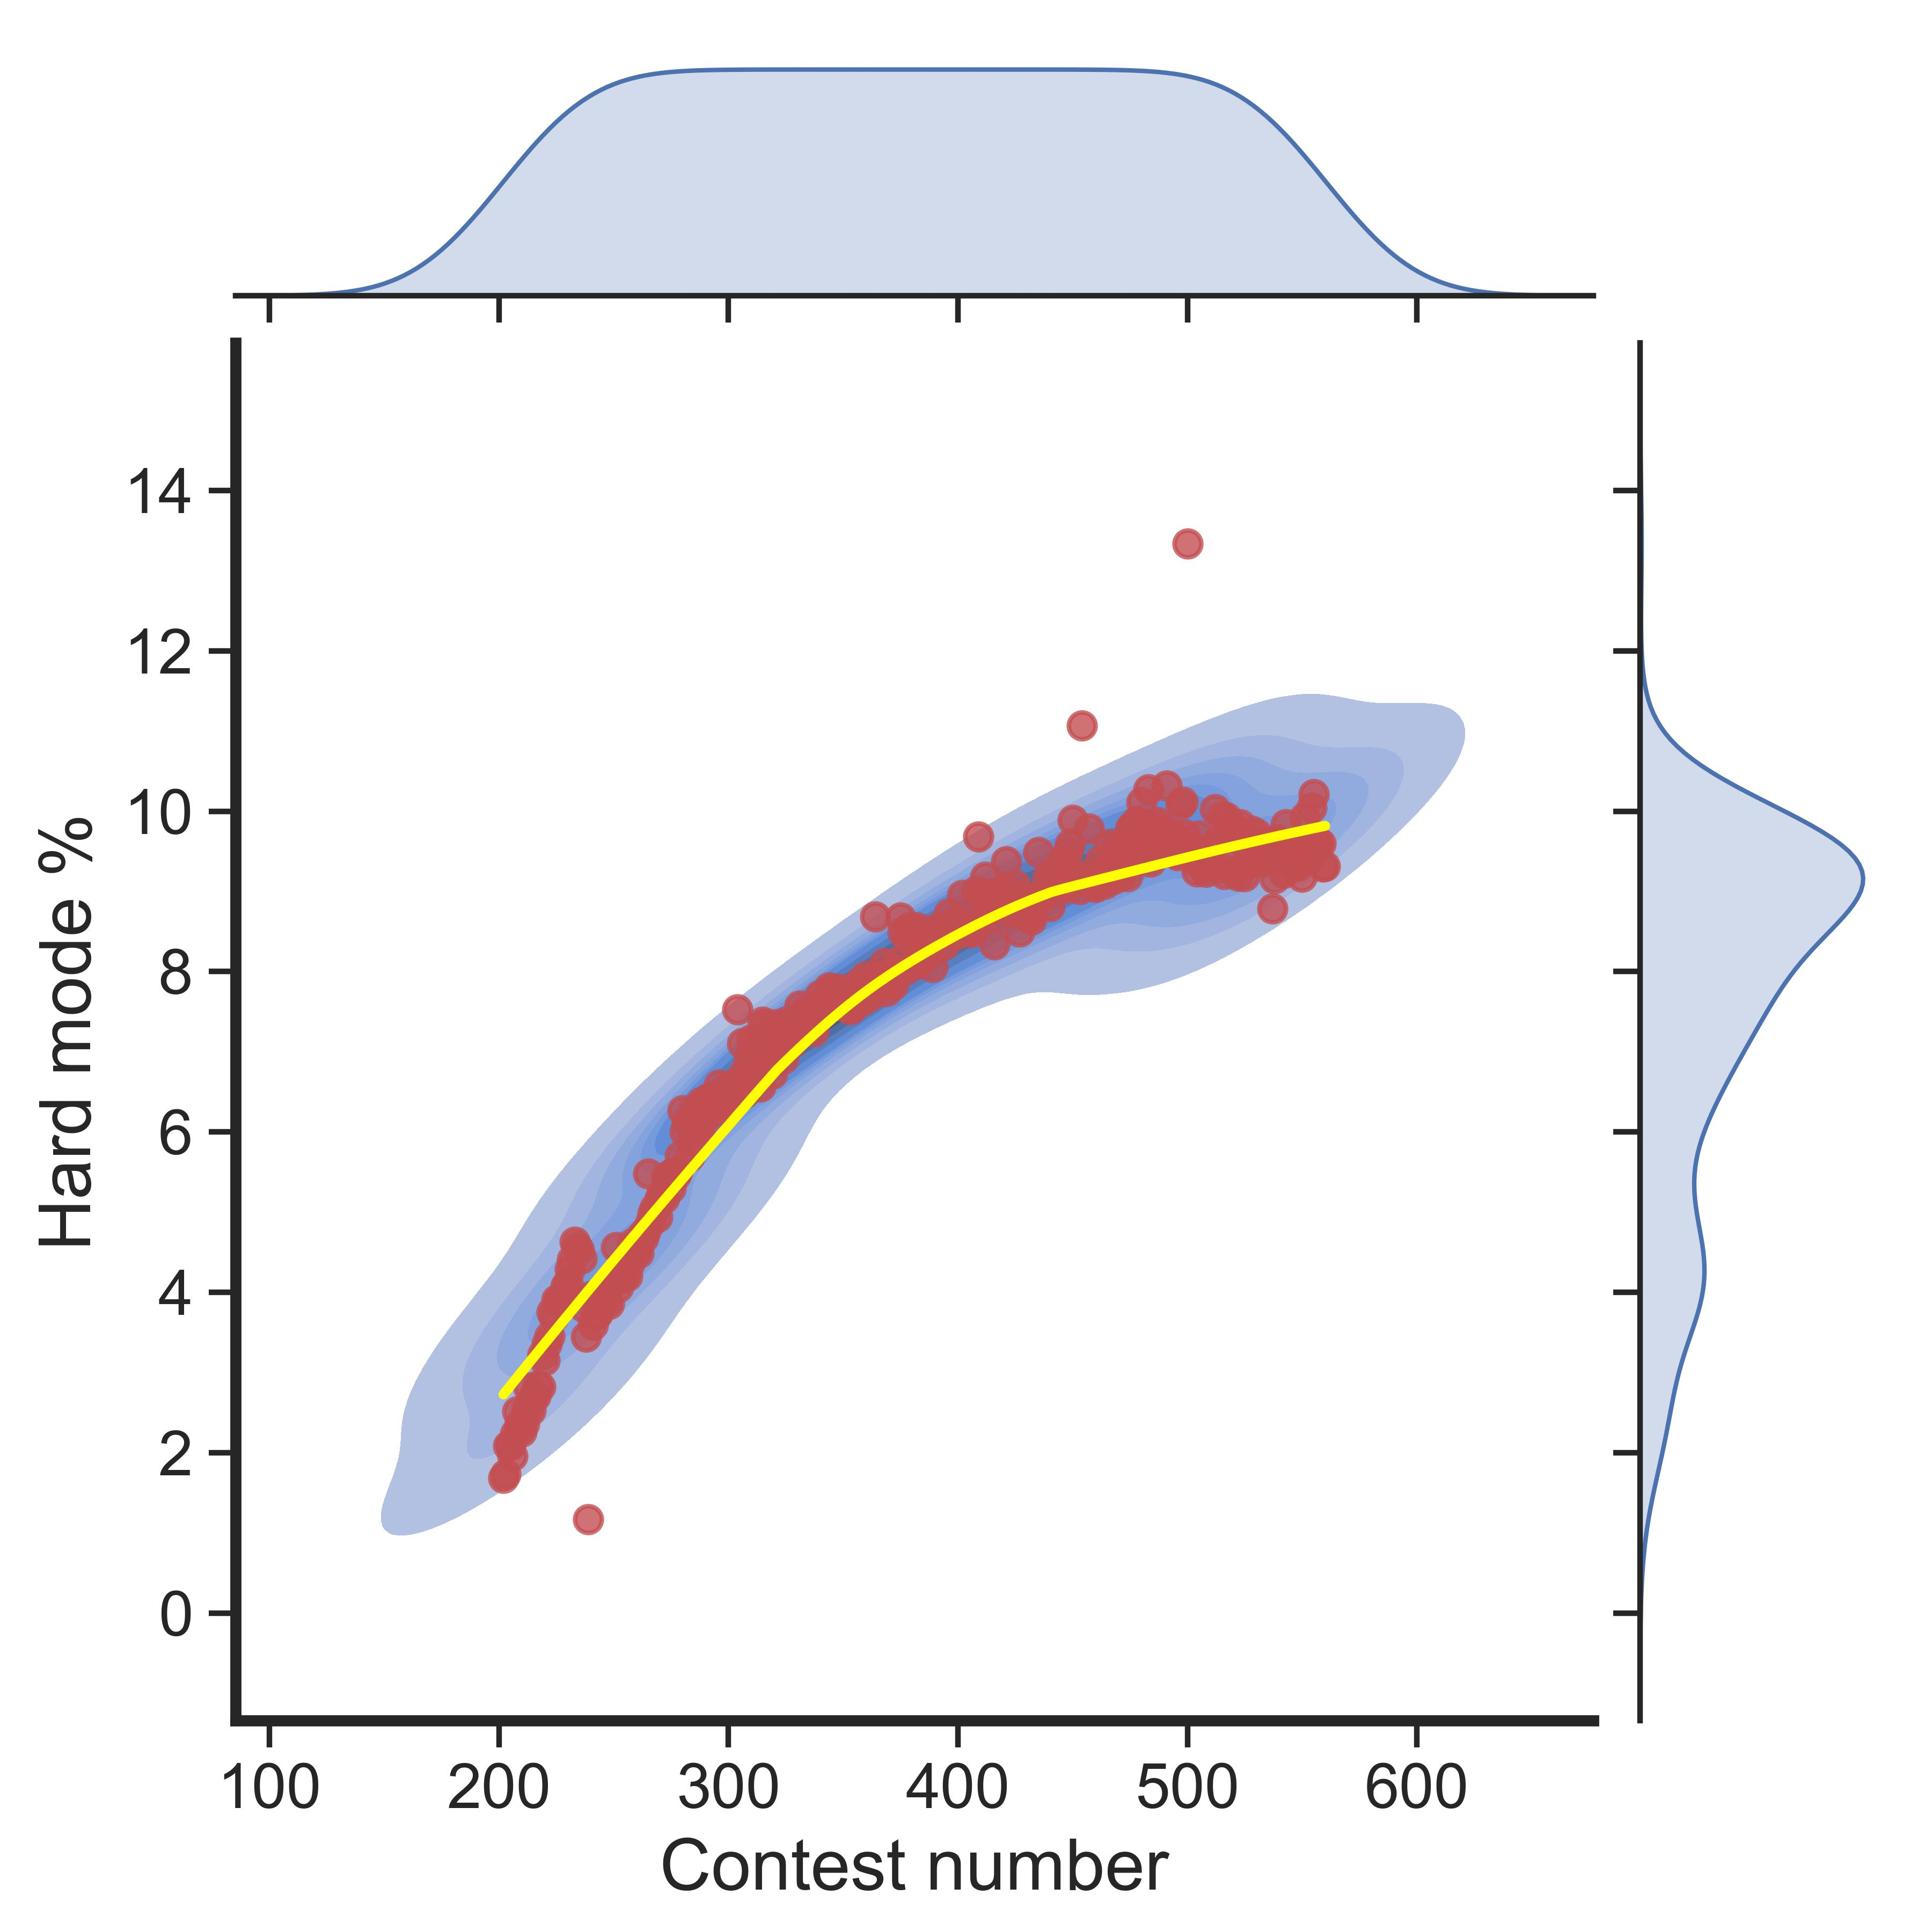
\includegraphics[scale=0.35]{hard_mode_kde.jpg}
		\end{minipage}
	} \quad \quad \quad \quad \quad \quad \quad 
	\subfigure
	{
		\begin{minipage}[b]{.28\linewidth}
			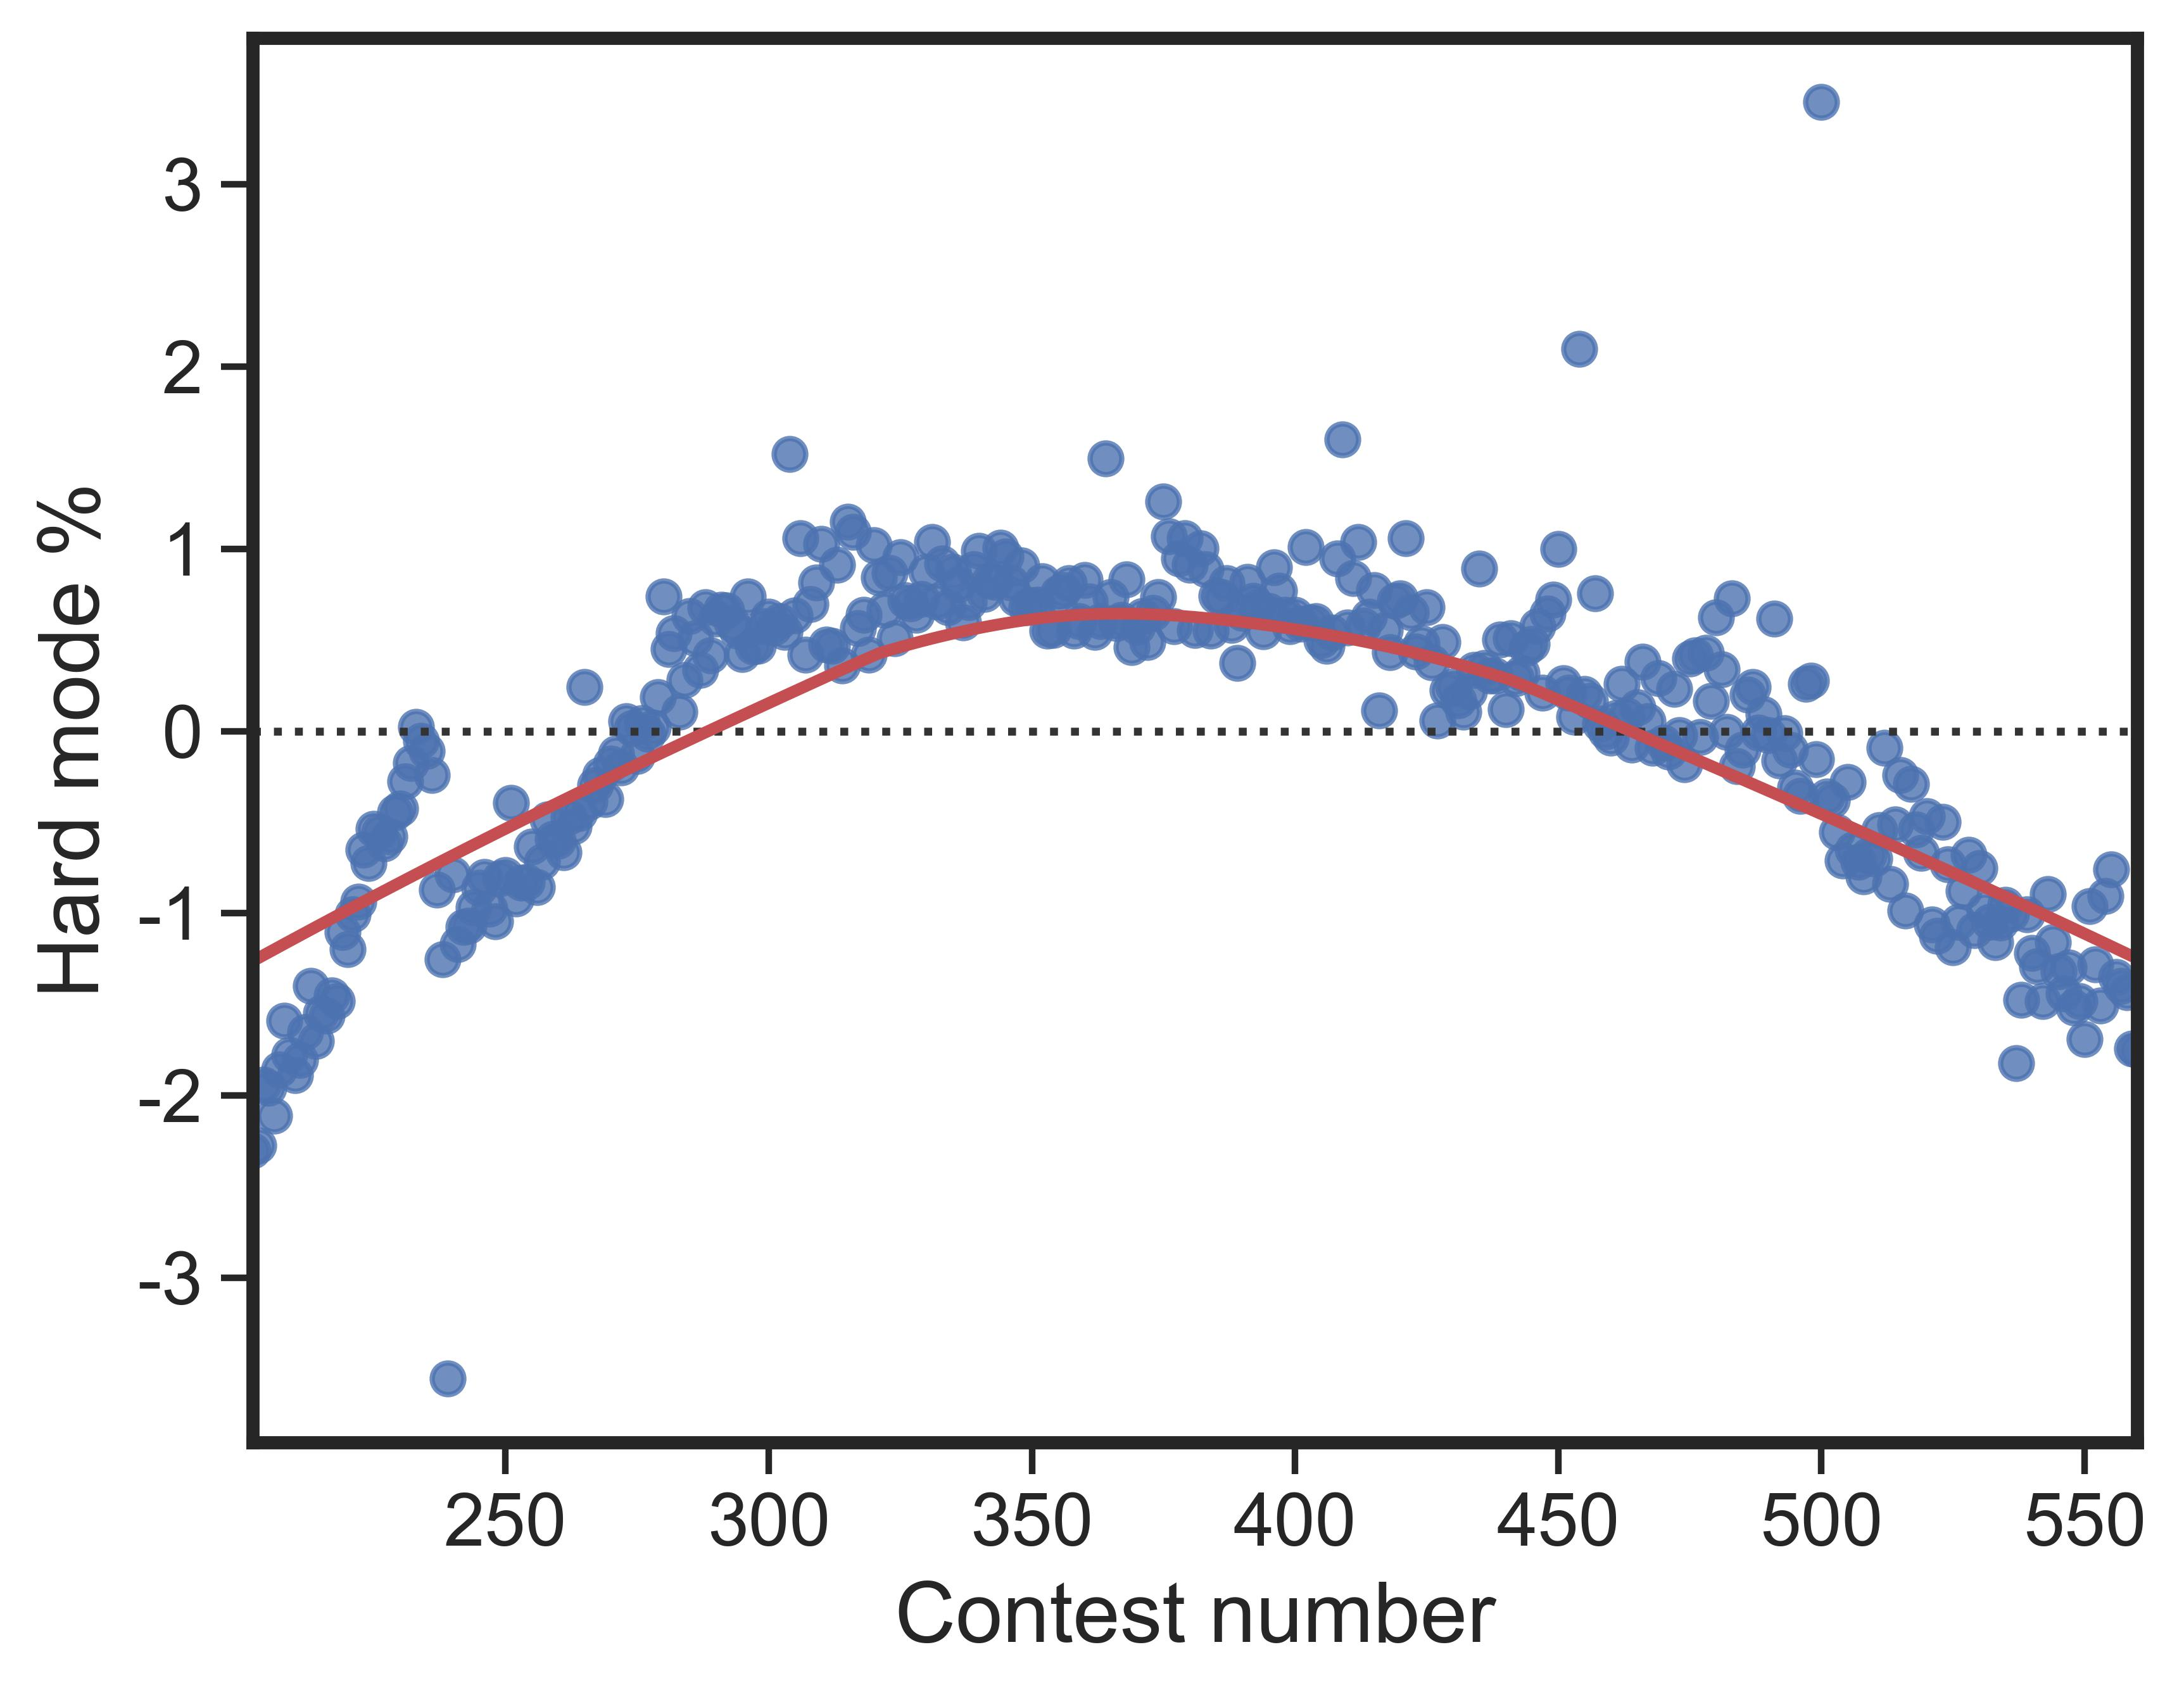
\includegraphics[scale=0.35]{hard_mode_resid.jpg}
		\end{minipage}
	}
\end{figure}
 \noindent
\textbf{6.2 Part of speech has no effect on difficulty}

We analyze the parts of speech of the given words. Part of speech symbols and frequency of occurrence are listed in appendix.

By counting the occurrence times of these parts of speech, the parts of speech and difficulty are analyzed, and the boxplot is drawn. It can be found that the parts of speech and difficulty are not necessarily related.
\begin{figure}[H]
	\centering
	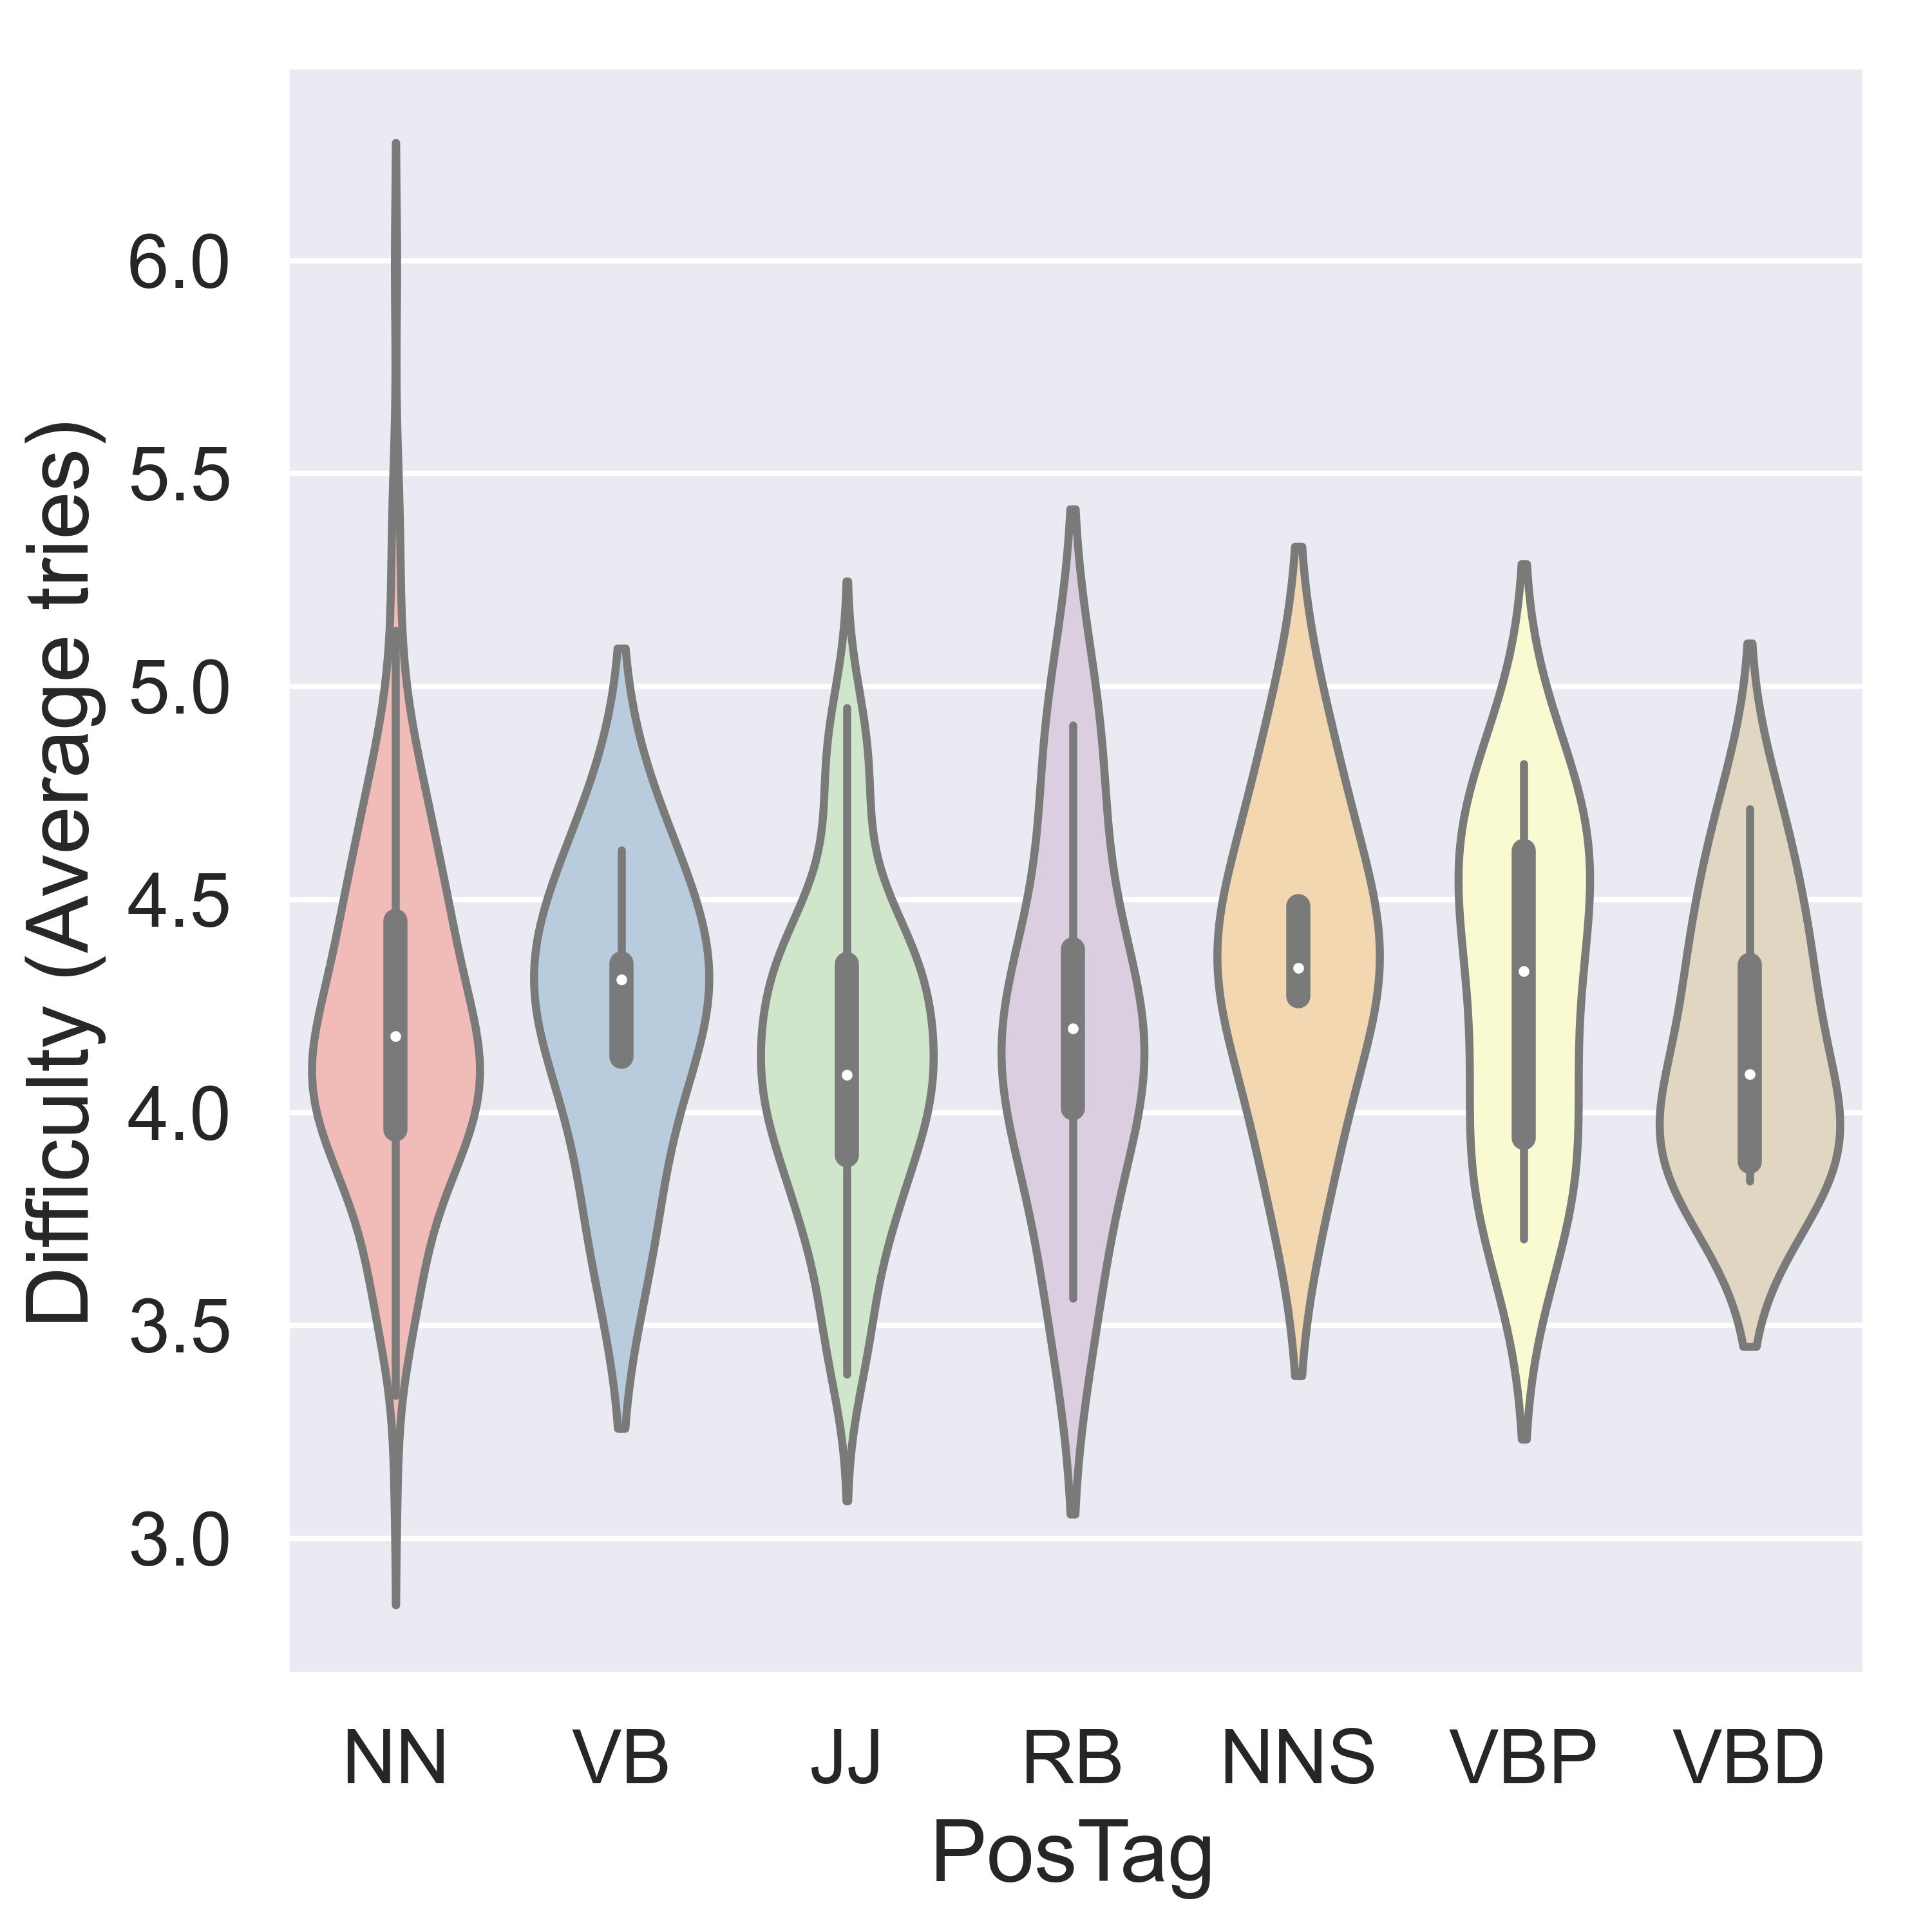
\includegraphics[width=.35\textwidth]{Q4_1.jpg}
	\caption{\small Comparison of difficulty of PosTag}
\end{figure}
 \noindent
\textbf{6.3 The number of letters in the puzzle will affect the whole difficulty}

By counting the number of letters, when the letters 'a,h,i,n,p,r,s,t' appear in the riddle word, the overall difficulty will become simpler.The difficulty becomes harder when 'b,g,j,k,q,v,w,x,y,z' occur in words.
\begin{figure*}[htbp] %通栏
	\begin{minipage}[t]{0.33\linewidth} %调节两个子图左右间距
		\centering
		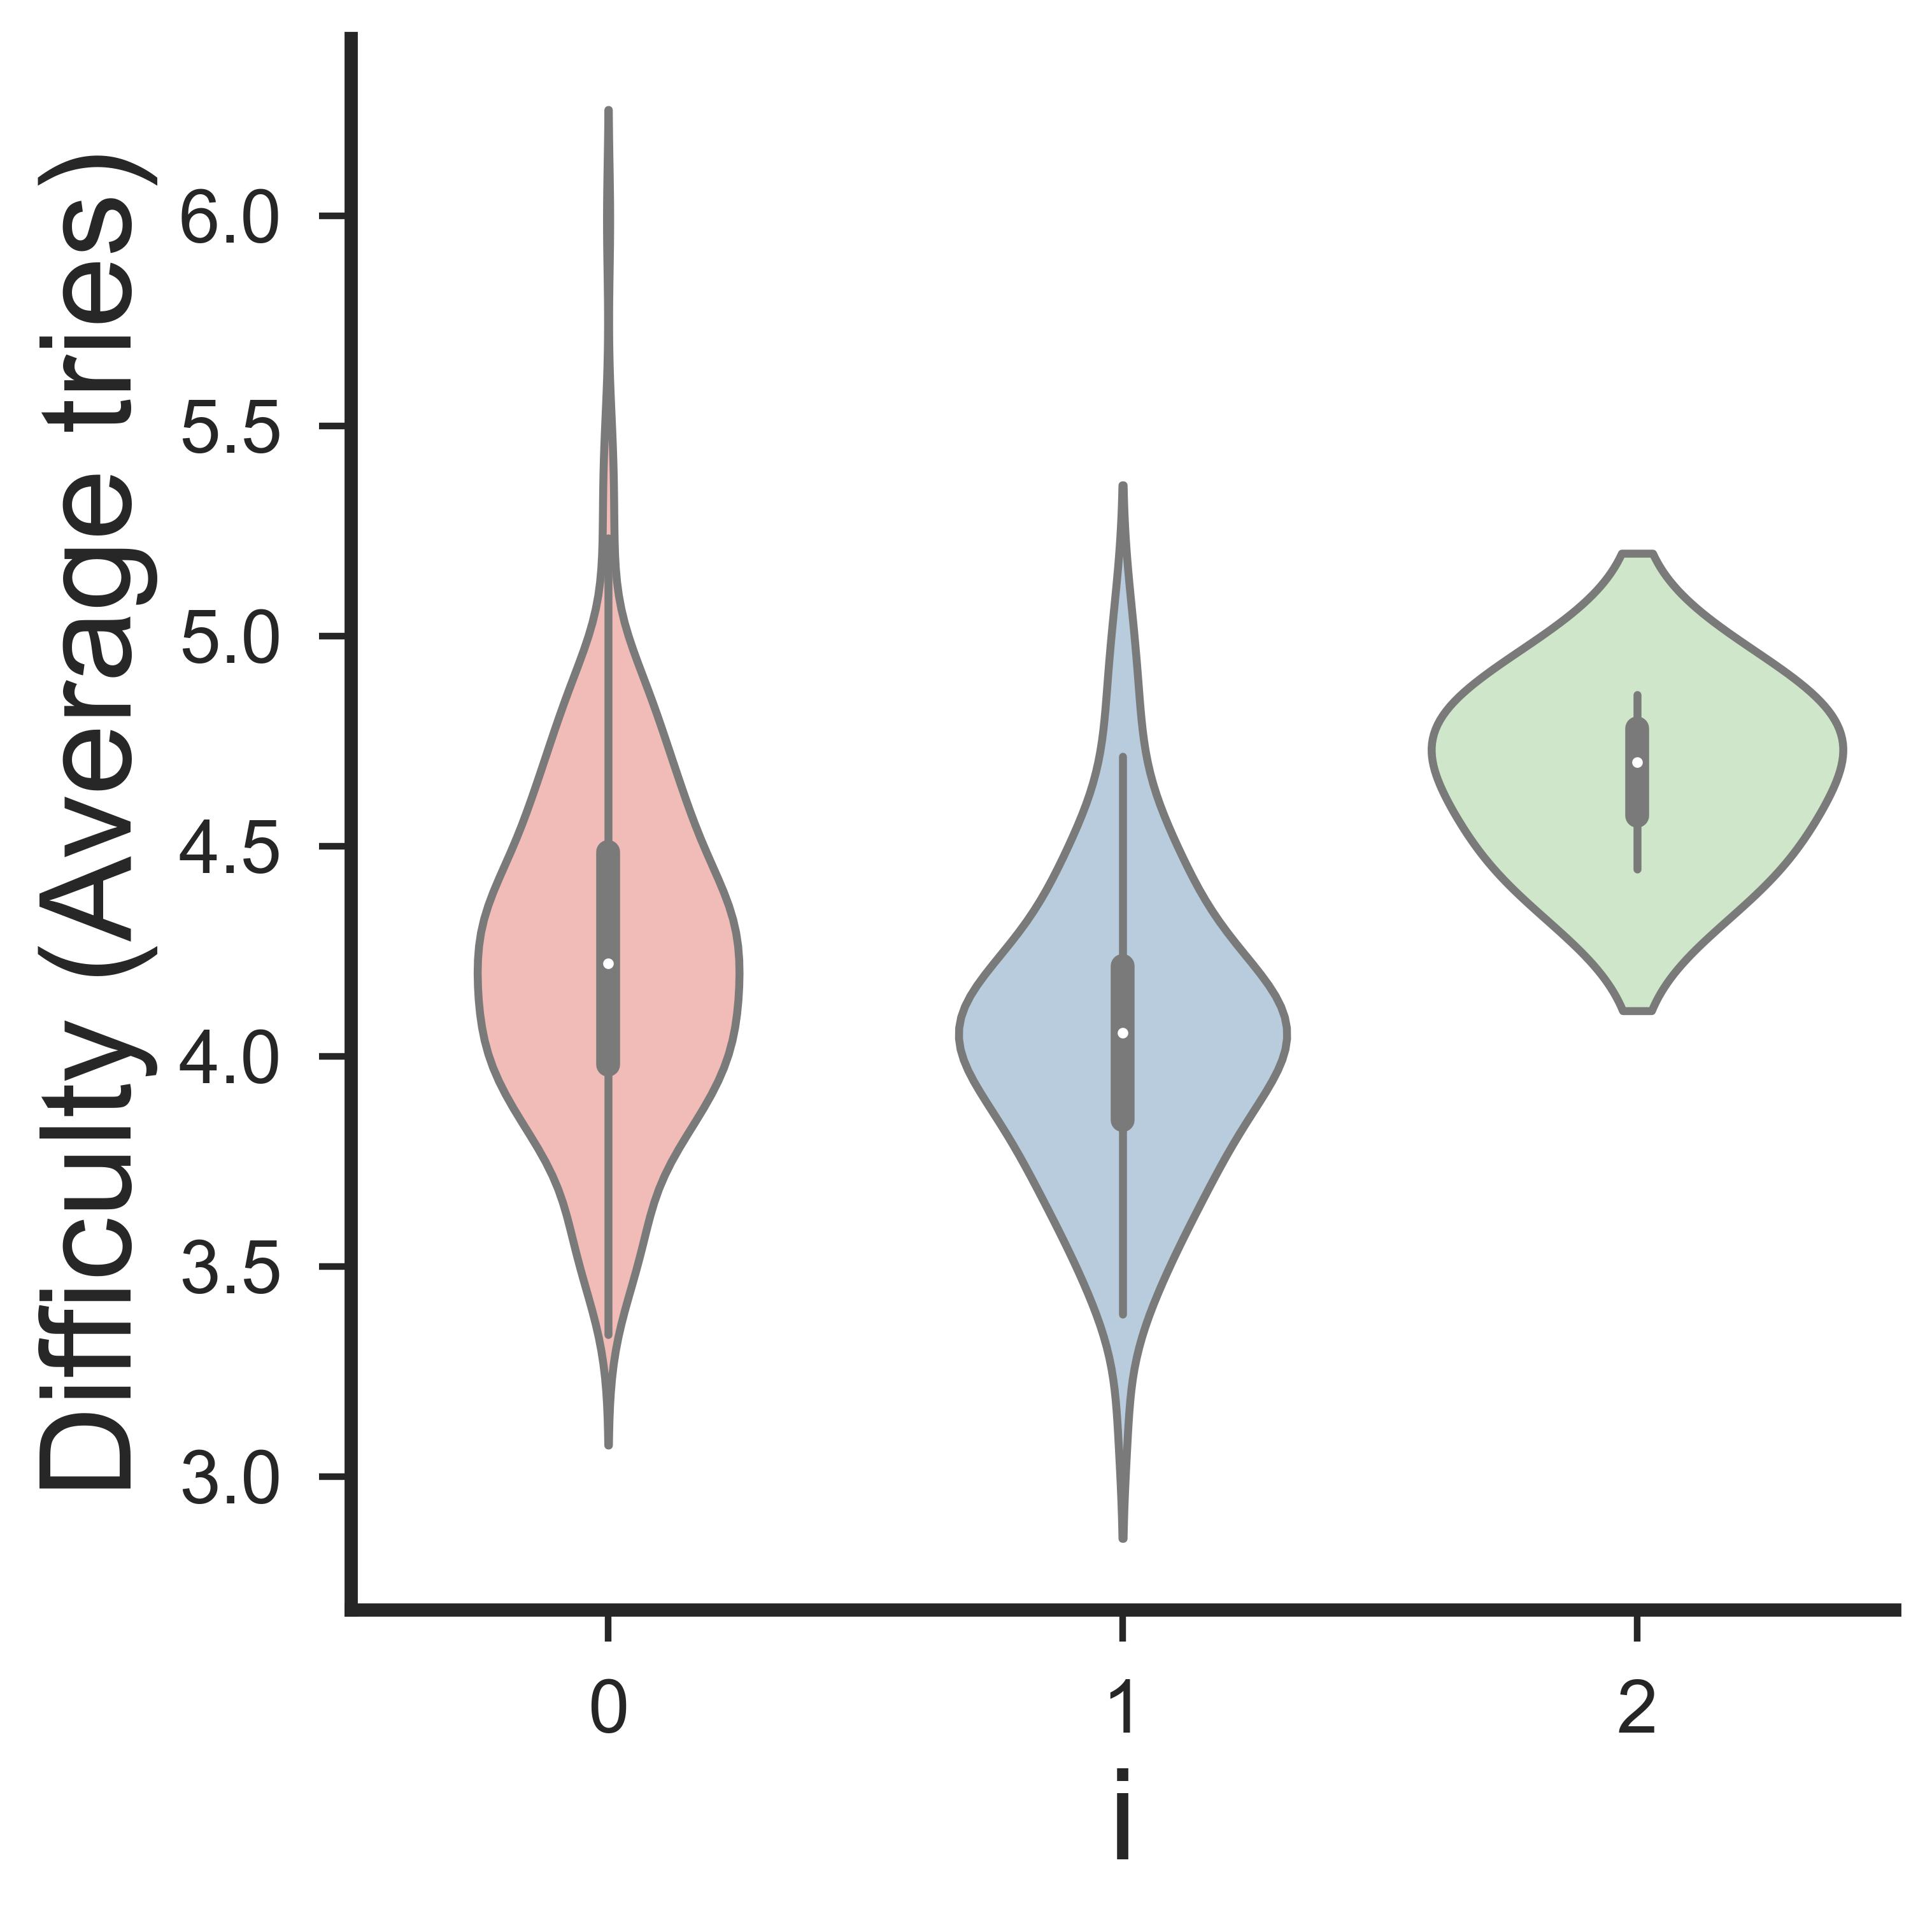
\includegraphics[width=1.9in, height=1.9in]{letter_i.jpg} %调节单个子图大小
	\end{minipage}%
	\begin{minipage}[t]{0.33\linewidth}
		\centering
		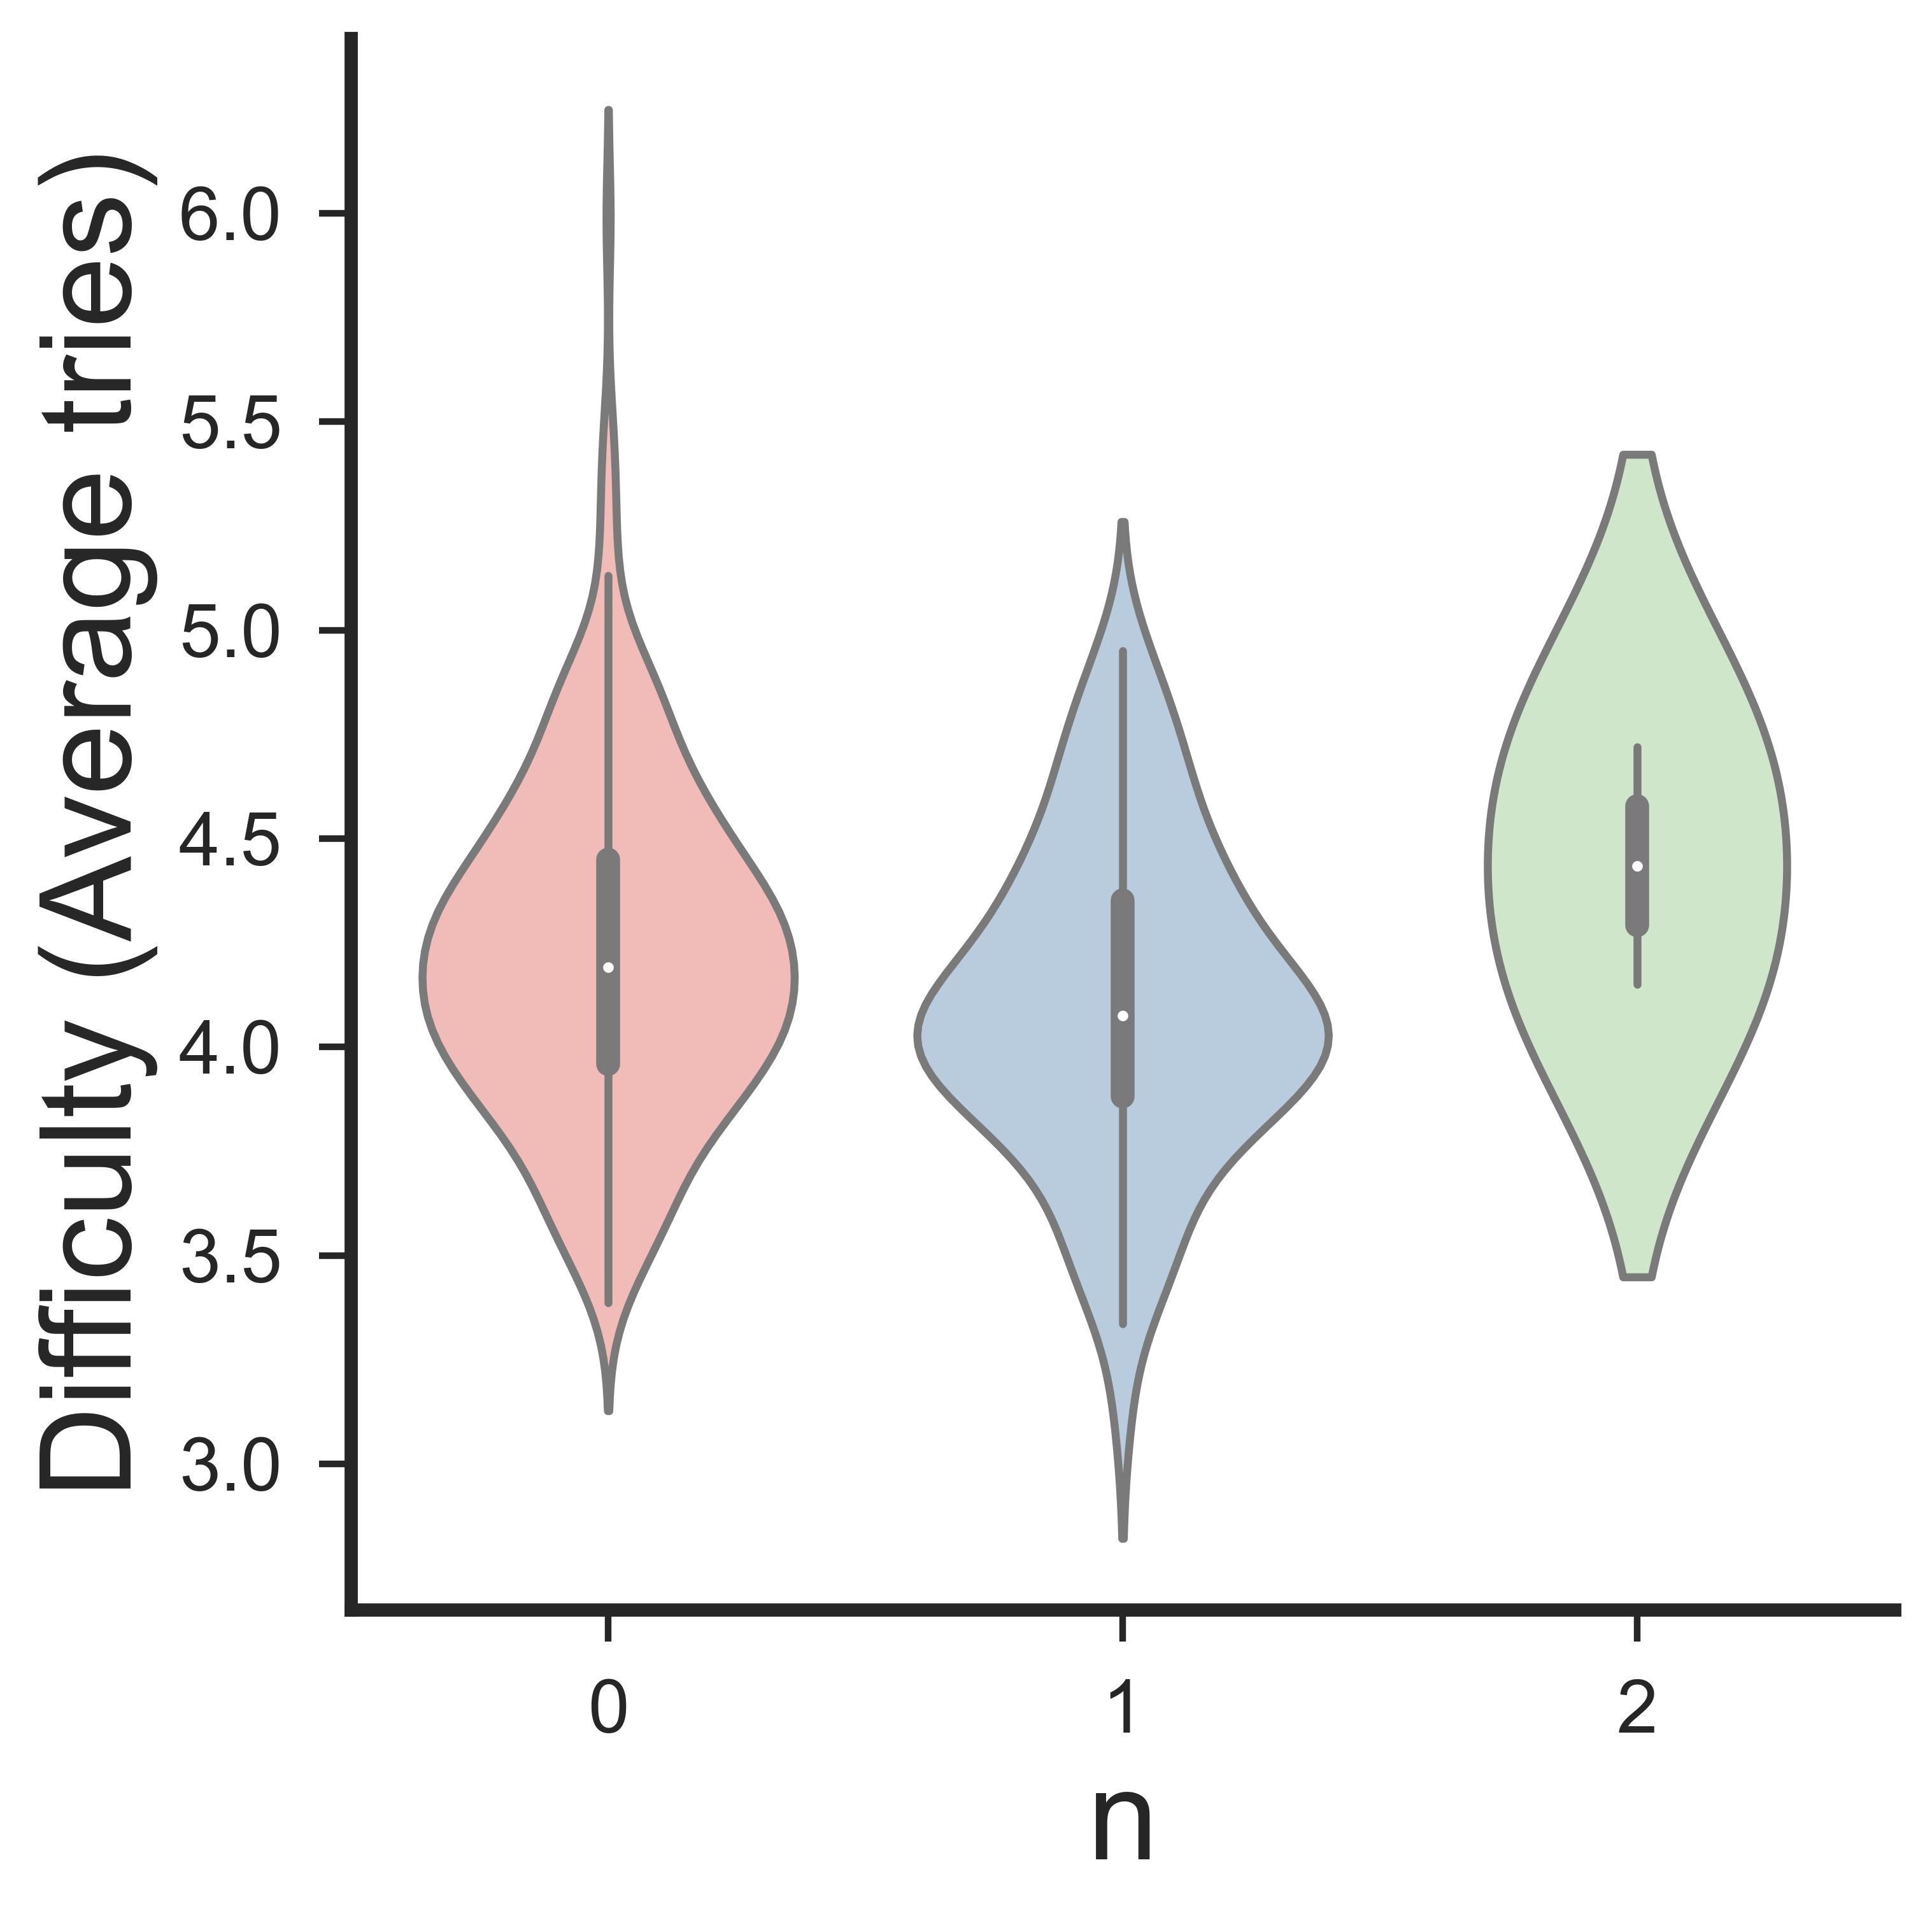
\includegraphics[width=1.9in, height=1.9in]{letter_n.jpg}
	\end{minipage}%
	\begin{minipage}[t]{0.33\linewidth}
		\centering
		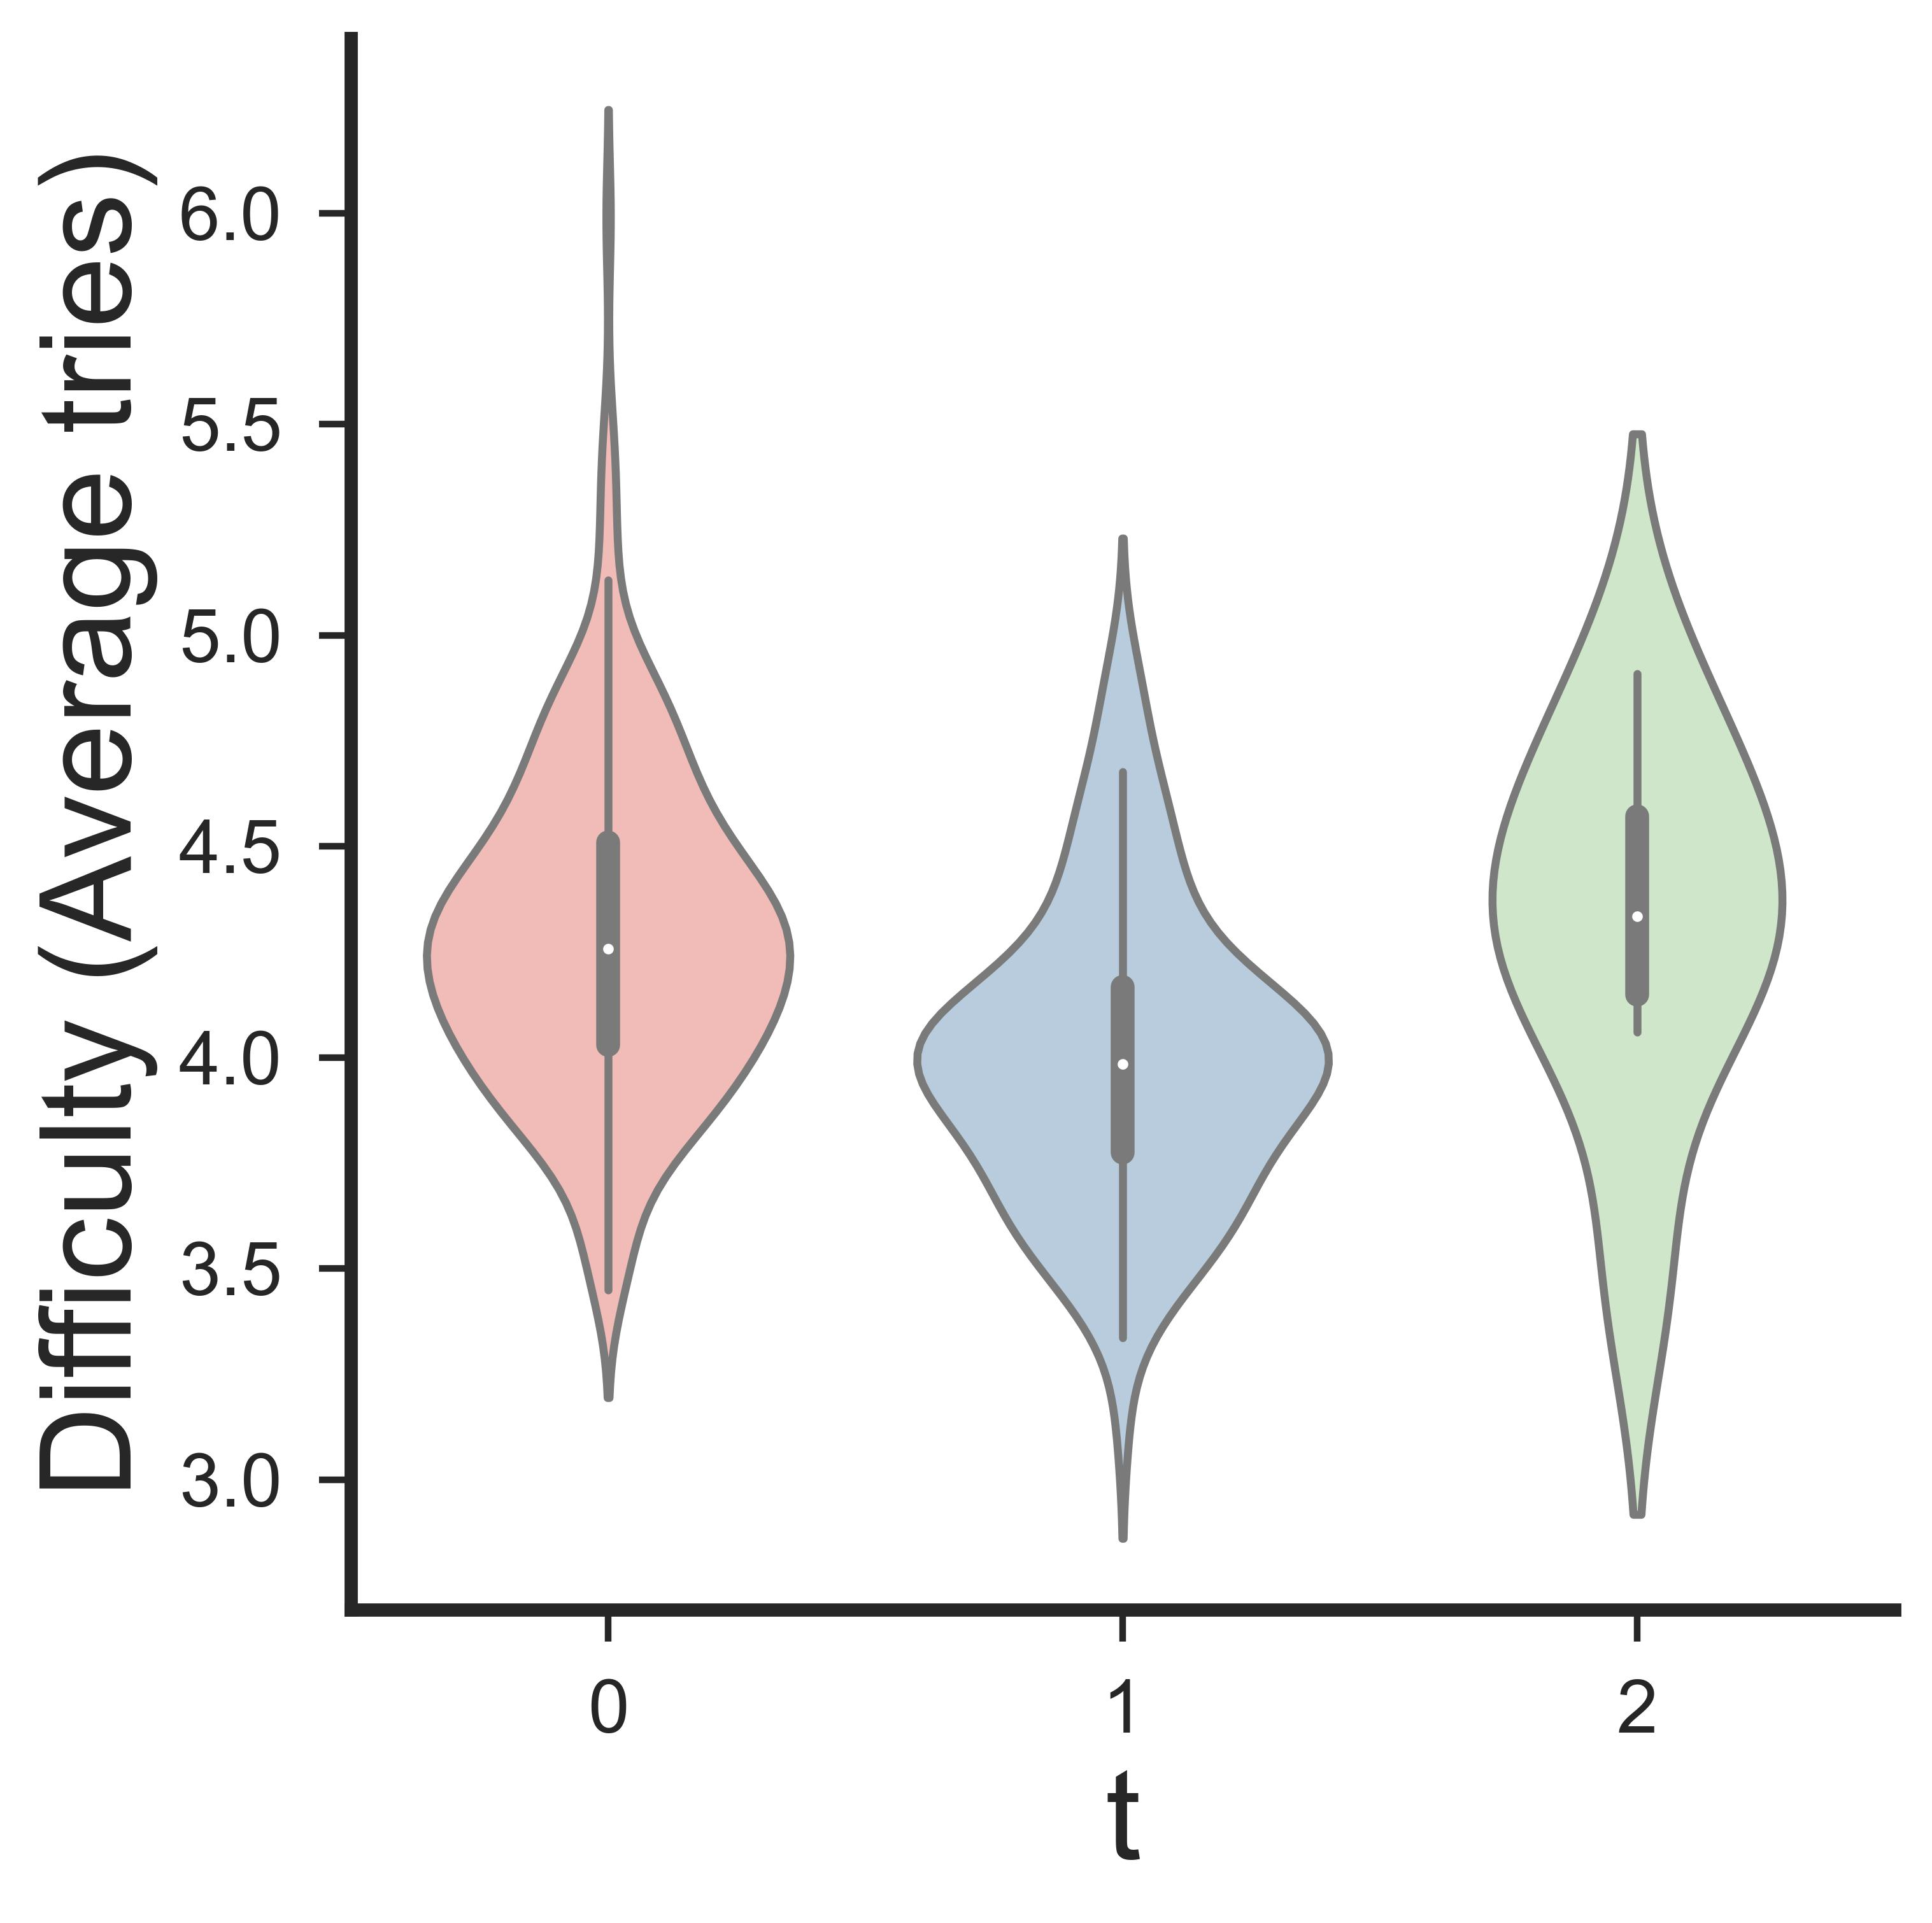
\includegraphics[width=1.9in, height=1.9in]{letter_t.jpg}
	\end{minipage}
\end{figure*}
\begin{figure*}[htbp] %通栏
	\begin{minipage}[t]{0.33\linewidth} %调节两个子图左右间距
		\centering
		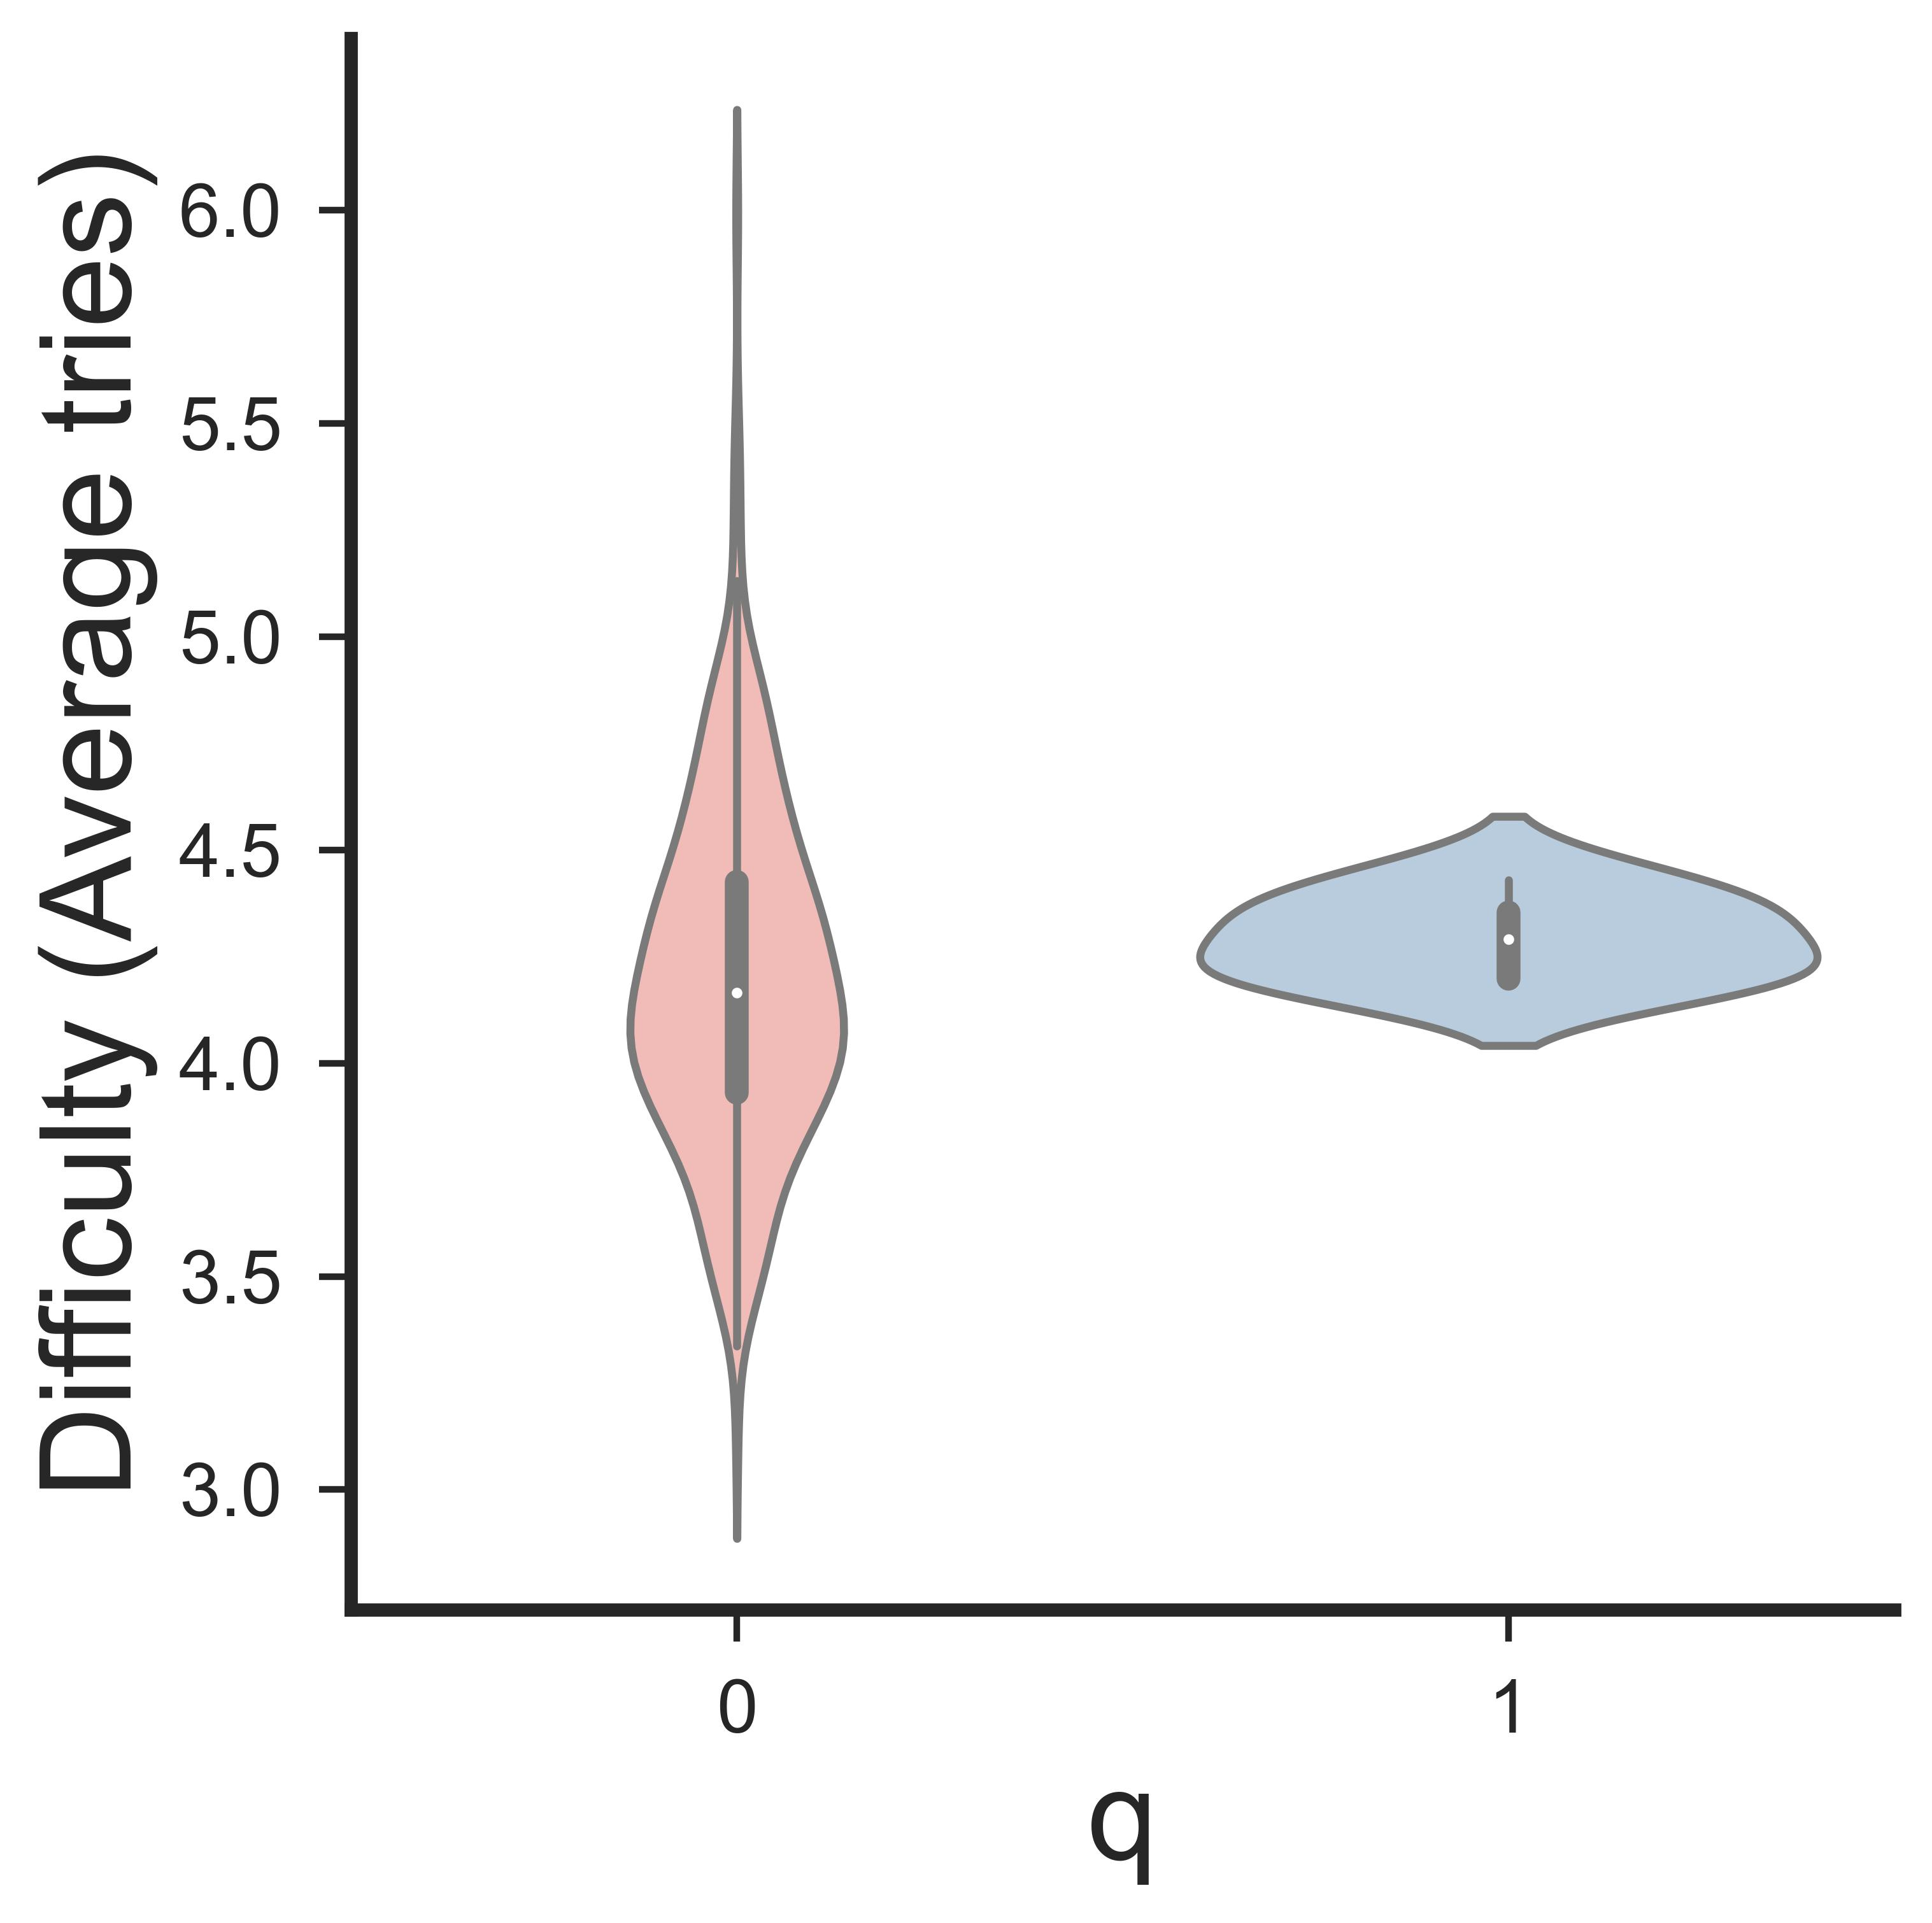
\includegraphics[width=1.9in, height=1.9in]{letter_q.jpg} %调节单个子图大小
	\end{minipage}%
	\begin{minipage}[t]{0.33\linewidth}
		\centering
		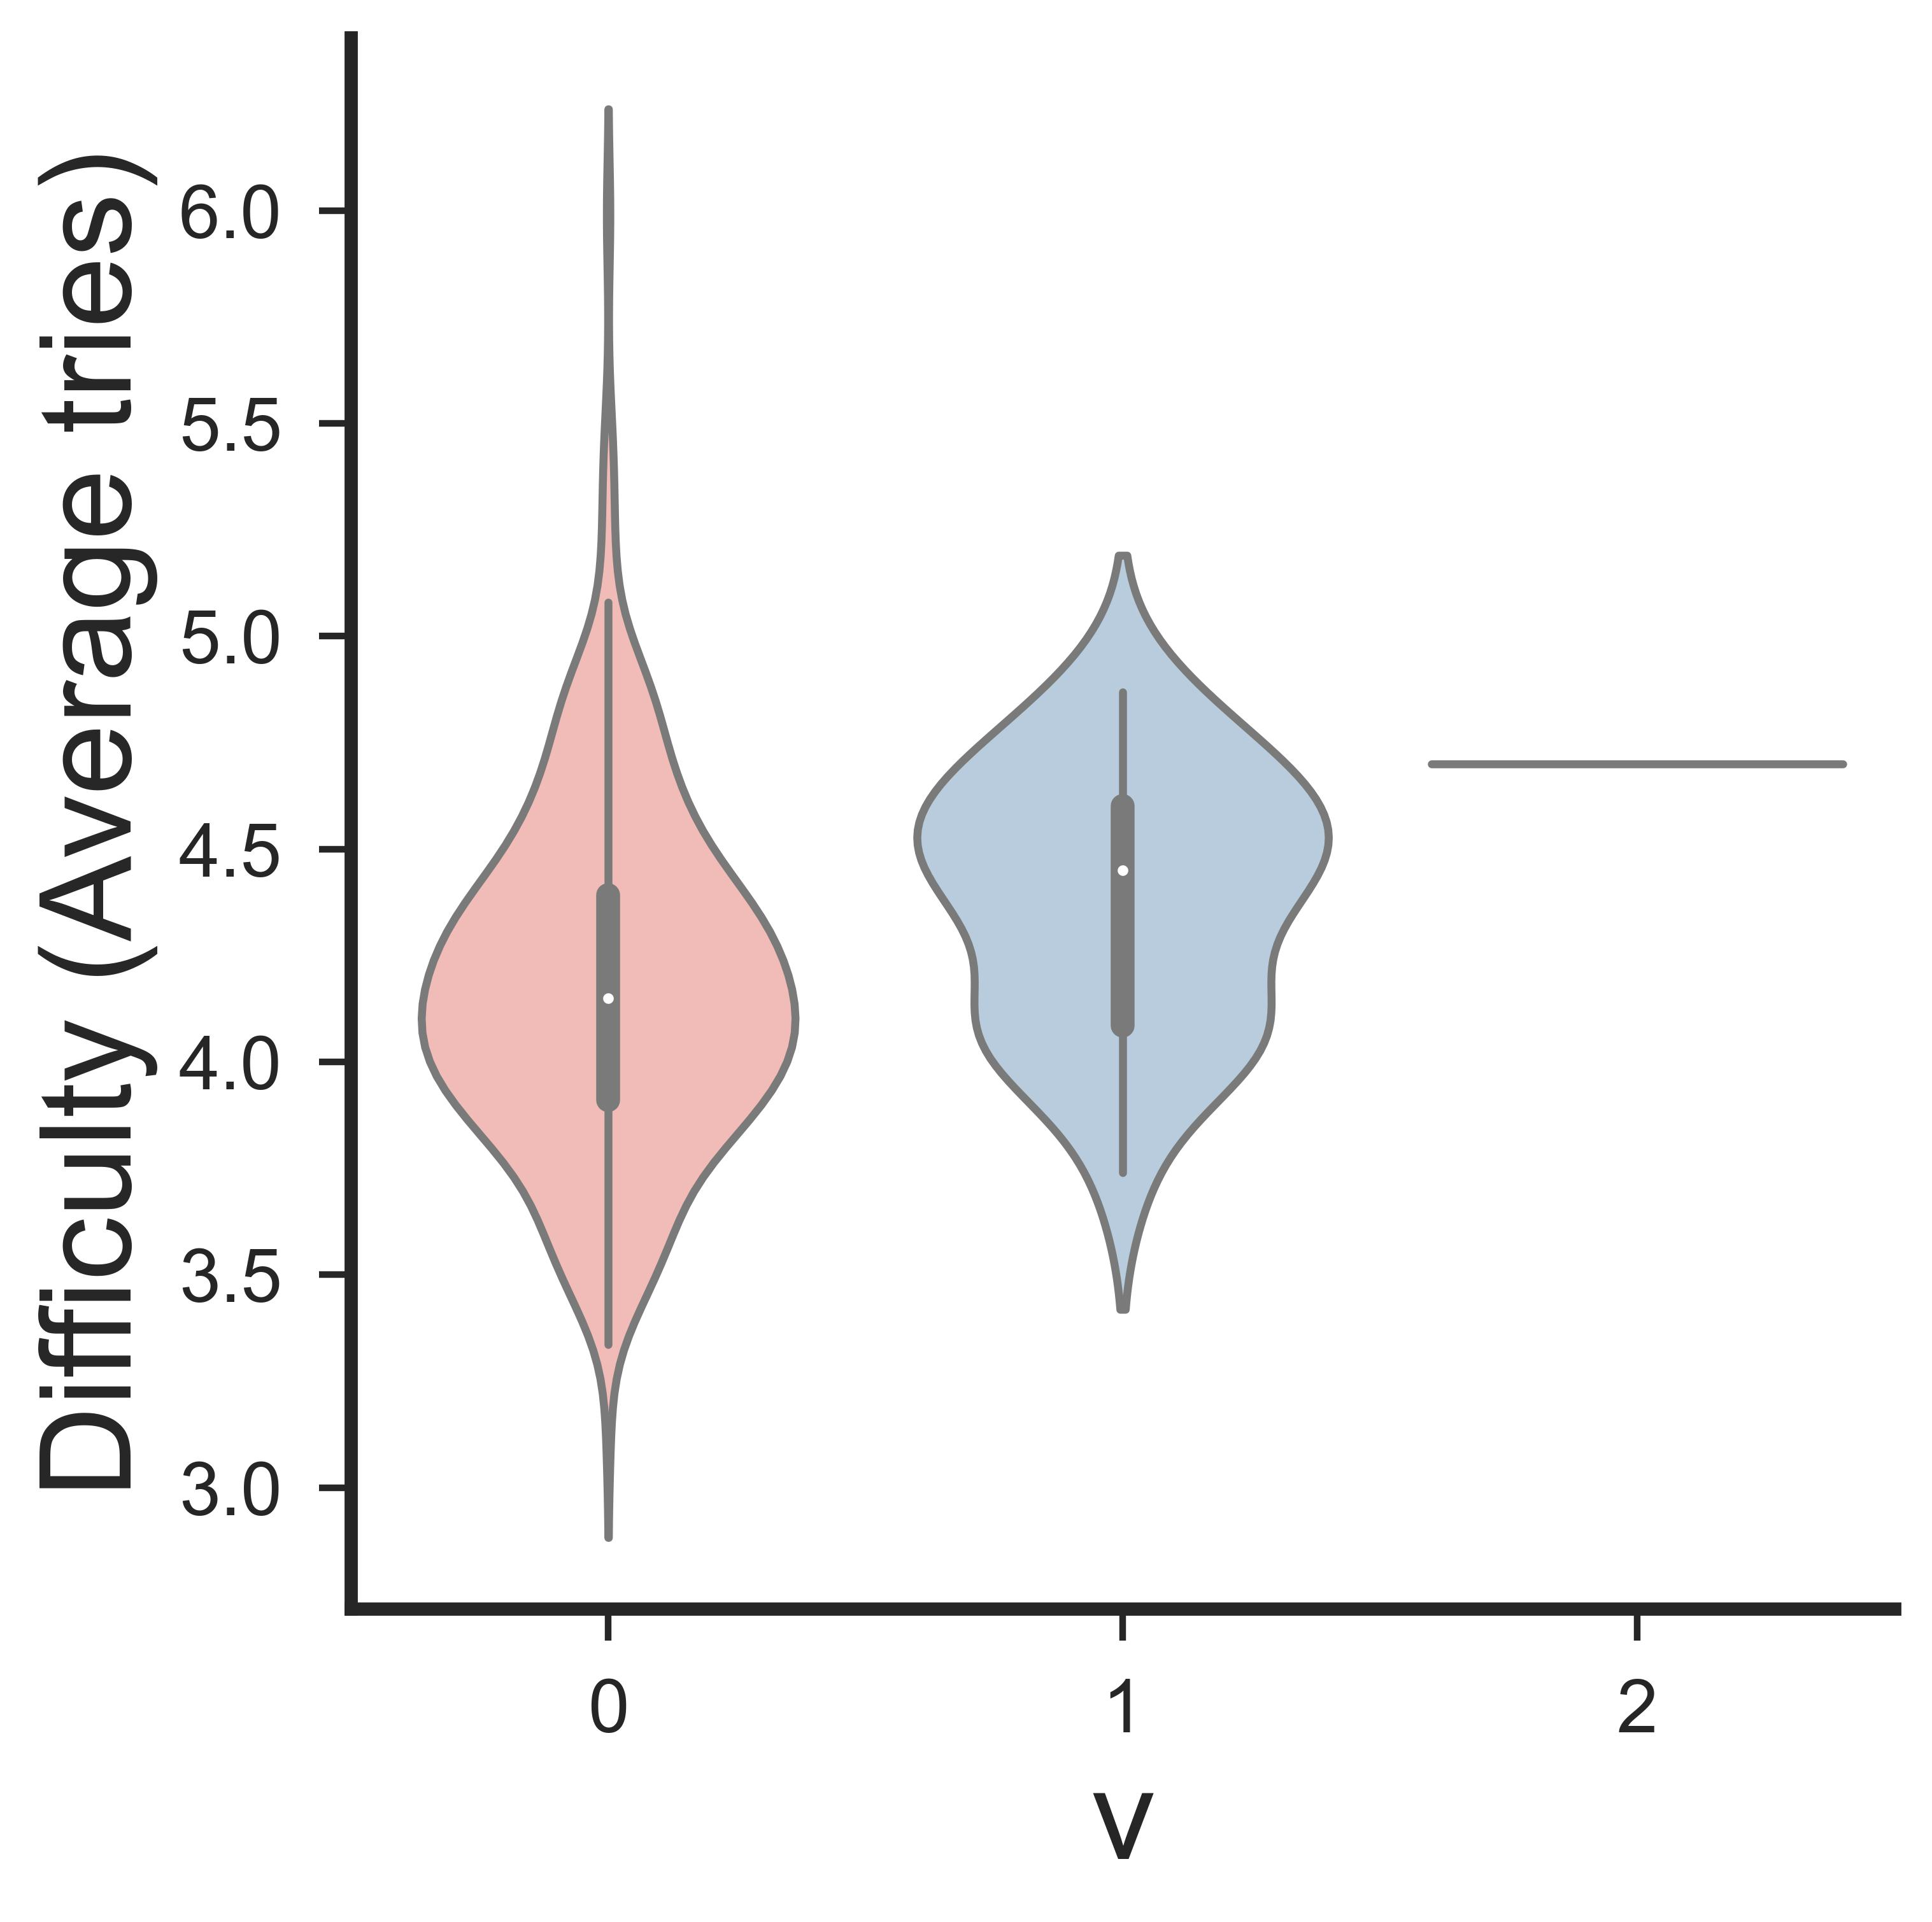
\includegraphics[width=1.9in, height=1.9in]{letter_v.jpg}
	\end{minipage}%
	\begin{minipage}[t]{0.33\linewidth}
		\centering
		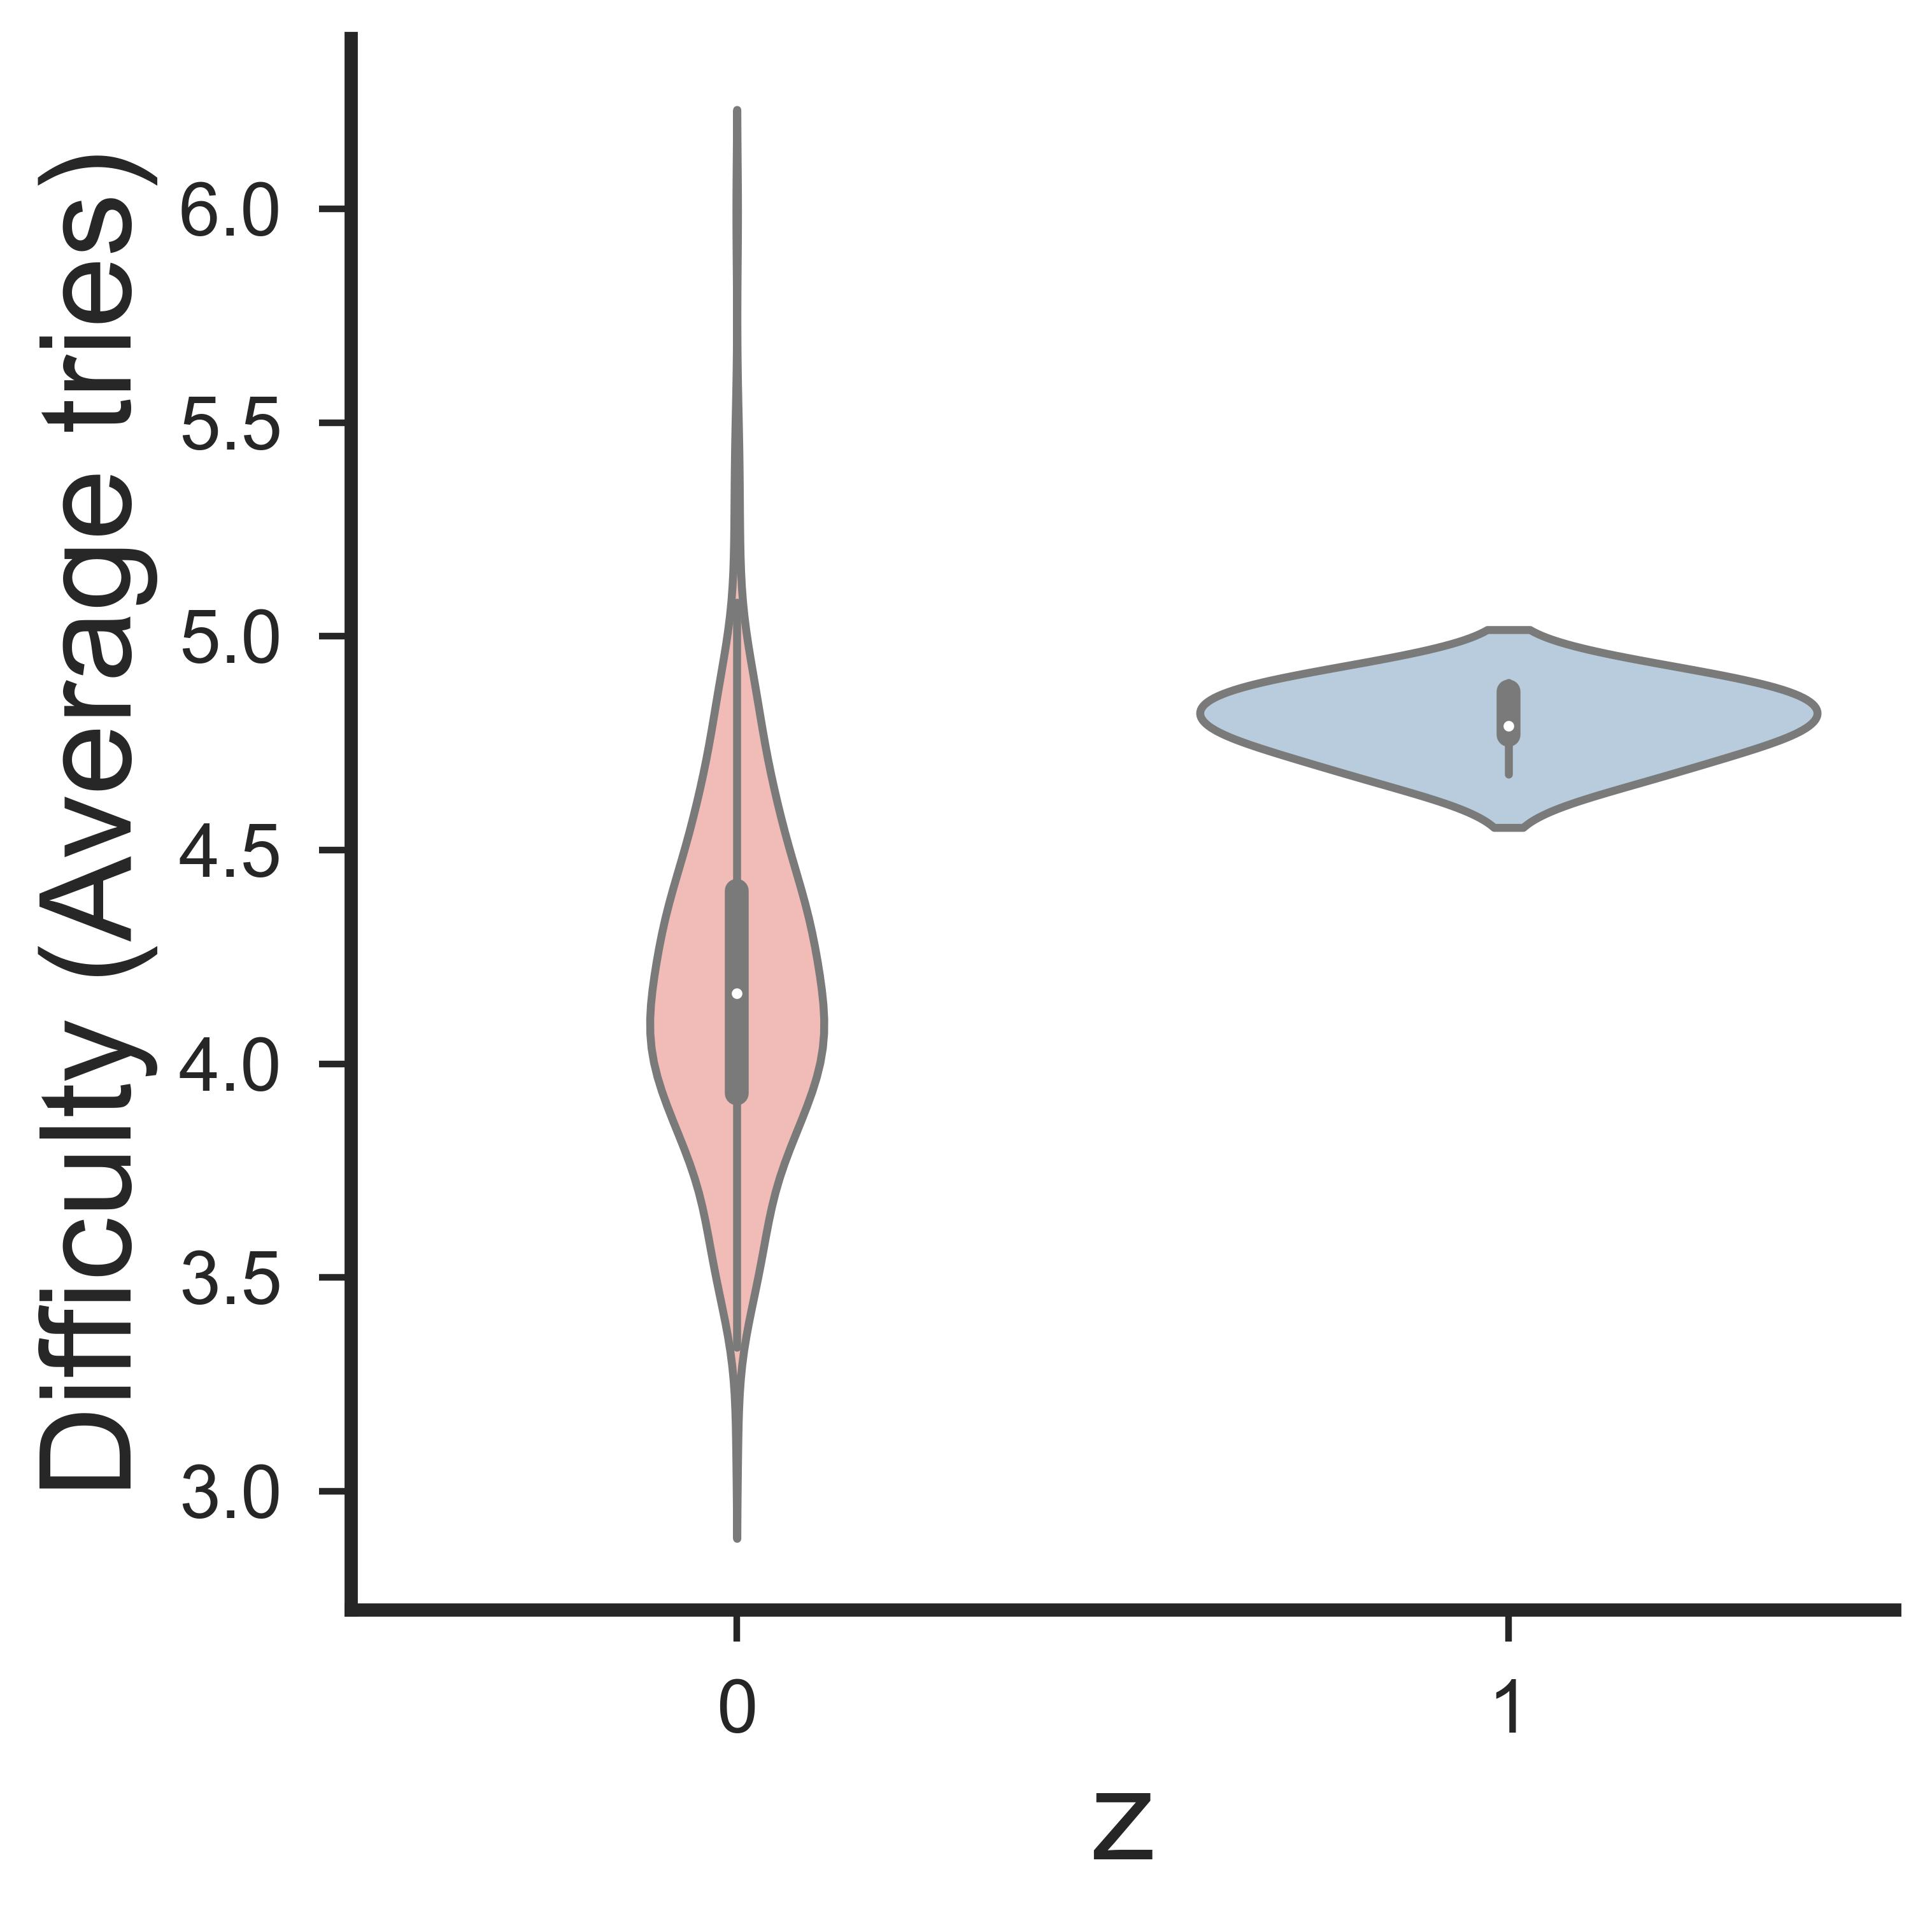
\includegraphics[width=1.9in, height=1.9in]{letter_z.jpg}
	\end{minipage}
\end{figure*}
\section{Conclusion}

\subsection{Strengths}
\begin{itemize}
\item Because of the volatility of the data, the traditional time series model cannot be used for analysis. Therefore, based on the complex network communication dynamics model, this paper explains the data volatility by using Twitter information transmission rate, user publication rate and other factors. Accurately predict the range of the number of reported results in the future.
\item With various word features as independent variables, multiple stepwise regression was used to model the percentage of attempts. Successfully predicted the release of EERIE scores.
\item Combining with information theory, word features are divided into objective conditions such as information entropy, popularity and letter combination to make the model more specific and comprehensive.
\item Using K-means clustering algorithm, cluster analysis was conducted on the percentage of attempts. Define the difficulty type according to the classification result. BP neural network was used to construct a difficulty evaluation model with the number of attempts as independent variable and difficulty as dependent variable.
\end{itemize}

\subsection{Possible Improvements}
Our model has the following limitations and related improvements
\begin{itemize}
	\item When calculating the attributes of word information entropy, word usage frequency can be added to optimize the calculation mode of information entropy, so that the result is more matching with the reality.
	\item When establishing the information propagation model, some optimization algorithms such as neural network can be combined to further optimize the parameters.
	\item If we had more complete data, we could add variables of player characteristics to the prediction of percentage of attempts, which would be more accurate.
\end{itemize}

Undeniably, in order to ensure the accuracy of prediction results as much as possible, this paper uses a variety of data about the attributes of words that can be collected, among which there must be some influencing factors that we have not taken into account that may cause deviations between model results and future actual values.

\begin{thebibliography}{99}
\bibitem{1} Huan Liu; Qing Bao; Hongjun Qiu; Ming Xu; Benyun Shi. 2021. Source Identification of Asymptomatic Spread on Networks.
\bibitem{2}Zhongdong Yin; Junye Cheng. 2023. Distribution transformer winding material identification algorithm based on Kmeans clustering.
\bibitem{3}Imran, H.; Al-Abdaly, N.M.; Shamsa, M.H.; Shatnawi, A.; Ibrahim, M.; Ostrowski, K.A. 2022. Development of Prediction Model to Predict the Compressive Strength of Eco-Friendly Concrete Using Multivariate Polynomial Regression Combined with Stepwise Method.
\bibitem{4}Koponen I; Södervik I. 2022. Lexicons of Key Terms in Scholarly Texts and Their Disciplinary Differences: From Quantum Semantics Construction to Relative-Entropy-Based Comparisons.

\end{thebibliography}

 \newpage
  \begin{memo}[Memorandum]
 \noindent
 \textbf{Dear Puzzle Editor of The New York Times,}
 
 Wordle, a free word-guessing game, has taken the world by storm, with more than 2 million players worldwide. In our opinion, as a small game with simple style, the five-character words preset by the system every day are not only the only puzzle of the day, but also the breakthrough of Wordle's viral spread. Players only need to spend a few minutes to complete the game every day, which effectively strengthens the "sense of scarcity" of the game experience.
 
 After our research, we are not worried about the total number of words used as puzzles at first. The total number of five-character words is more than 12,000, excluding rare words, the range of game answers can still reach about 2,500, and such a vocabulary bank can last for nearly seven years. So our research is more about distinguishing the specific properties of words for games. Combined with word frequency, information entropy and other data, we established a unique evaluation model, which can effectively evaluate the difficulty of guessing words as the answer to riddles quantitatively. It can also predict roughly how well the player will answer the riddle.
 \begin{figure}[H]
 	\centering
 	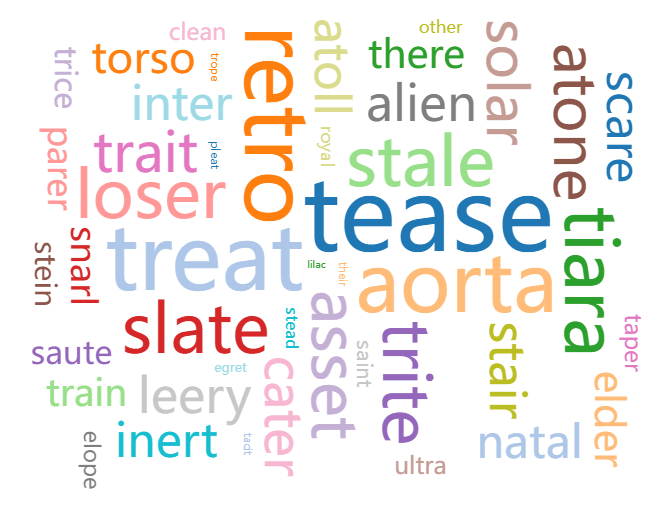
\includegraphics[width=.55\textwidth]{ ciyun.png}
 \end{figure}

We analyzed the mystery of 2022 for an entire year. Based on feedback from players, the most difficult word is parer on September 16, while the least difficult word is train on May 4. We also combined the complex network communication theory to construct a prediction model with a high degree of fit for the number of reports, trying to explain the small fluctuations in the number of reports over the past year. To some extent, the number of reports also reflects the number of game players, which can provide some reference value for the development of the game.

 Based on the above research, we have the following suggestions for the running of games and the selection of riddle words:
 
 \textbf{1. Select words with large differences in difficulty coefficients on adjacent days}
 
 Developers have a certain amount of information guidance, and can use the data of player feedback on various social platforms to describe a certain amount of player experience. In turn, changes can be made to the player experience. When the majority of players said the answer to the riddle was easy, the more difficult word was chosen as the answer, and vice versa. Maximize the player experience and thus increase the engagement of game players.
 
 \textbf{2. Develop multiple game modes to give players more options based on word attributes}
 
 As the current game tips are more in the process of player speculation, for the player's different choices to give hints. Before the game started, there were only easy and hard modes, and the difference between the existing modes was that the difficulty was set more in the guessing process, rather than giving different players more freedom to accumulate words in different directions. Therefore, we want to create more game modes to provide some bias to the puzzle according to the player's preference. For example, some hints are given about the properties of the riddle word, the noun pattern, the verb pattern, or the fact that the riddle word is an animal, etc., so that players with different subjective preferences can have a better game experience.
 
\textbf{3. Give your game a longer life cycle with a little more hype}

Combined with the data, we found that the number of players for wordle has skyrocketed since its launch. Compared to other games of the same type, the achievement is very proud. However, by analyzing player data over the past year, it is clear that the total number of players has declined in the second half of the year. We think it probably has something to do with the fact that most people are starting to go back to work. Therefore, we suggest that while optimizing the word of the riddle, we should also increase the publicity of the game to ensure that more new players continue to flow in.

In the end, we hope that our research and related suggestions can help you in solving puzzles, and we sincerely hope that wordle will get better and better.

\vspace {3pt}
\rightline{Your Sincerely,}
\rightline{Team \#2300466}
 \end{memo}

 \newpage
\begin{appendices}
\begin{table}[H]
	\tabcolsep=12pt
	\centering
	\renewcommand\arraystretch{1.2}
	\caption{\small Model initial parameter}
	\par\medskip
	\begin{tabular}{cc}
			\hline
			Parameter &  Initial Value \\
			\hline
			N  & 4500000 \\
			\rowcolor[gray]{.85}
			$ \beta  $	& 0.2  \\ 
			$ \sigma $  & 0.1\\ 
			\rowcolor[gray]{.85}
			$ \gamma $	& 0.1 \\ 
			$ k $		& 3.3 \\ 
			\rowcolor[gray]{.85}
			$ z $   	& 0.25 \\
			\hline
		\end{tabular}
\end{table}
\begin{table}[H]
	\centering
	\caption{\small Classification of difficulty}
	\begin{tabular}{ccc}
		\toprule[1.5pt]
		\multicolumn{3}{c}{Degree of difficulty} \\  \midrule[1.5pt]
		\makebox[0.1\textwidth][c]{Easy} 
		& \makebox[0.1\textwidth][c]{Middle} & \makebox[0.1\textwidth][c]{Diffcult} \\
		$0\sim 3.43$    & $3.43\sim 4.8$      & $4.8\sim 5.99$    \\  \bottomrule[1.5pt]
	\end{tabular}
\end{table}
\begin{table}[H]
	\centering
	\caption{Part-of-speech statistics}
	\tabcolsep=12pt
	\small
	\renewcommand\arraystretch{1.1}
	\par\medskip
	\begin{tabular}{cll}
		\hline
		PosTag &  Description & Number  \\
		\hline
		NN  & noun singular & 205 \\
		\rowcolor[gray]{.85}
		JJ & adjective & 87 \\
		RB &  adverb & 13 \\
		\rowcolor[gray]{.85}
		VBP & The present tense of the non-third person singular & 12 \\
		VBD  & past tense & 10 \\
		\rowcolor[gray]{.85}
		VB & verb prototype &5 \\
		NNS & noun plural & 5 \\
		\rowcolor[gray]{.85}
		VBN & past participle of verb & 4 \\
		IN  & a preposition or subordinate conjunction & 3 \\
		\rowcolor[gray]{.85} 
		VBZ &  third person singular present tense & 3 \\
		VBG  & gerund or present participle & 3 \\
		\rowcolor[gray]{.85}
		MD & modal verb &2 \\
		CC  & joint conjunction & 2 \\
		\rowcolor[gray]{.85}
		PRP\$ &  possessive pronoun & 1 \\
		RBR  &  comparative adverb & 1 \\
		\rowcolor[gray]{.85}
		JJS & superlative adjective &1 \\
		DT  & qualifier &1 \\
		\rowcolor[gray]{.85}
		JJR & comparative adjective &1 \\
		\hline
	\end{tabular}
\end{table}

%\textbf{\textcolor[rgb]{0.98,0.00,0.00}{Input matlab source:}}
%\lstinputlisting[language=Matlab]{./code/mcmthesis-matlab1.m}

%\section{Second appendix}
%
%some more text \textcolor[rgb]{0.98,0.00,0.00}{\textbf{Input C++ source:}}
%\lstinputlisting[language=C++]{./code/mcmthesis-sudoku.cpp}

\end{appendices}
\end{document}

%% 
%% This work consists of these files mcmthesis.dtx,
%%                                   figures/ and
%%                                   code/,
%% and the derived files             mcmthesis.cls,
%%                                   mcmthesis-demo.tex,
%%                                   README,
%%                                   LICENSE,
%%                                   mcmthesis.pdf and
%%                                   mcmthesis-demo.pdf.
%%
%% End of file `mcmthesis-demo.tex'.
